\documentclass{report}

\usepackage[utf8]{inputenc}

\usepackage[
    backend=biber,
    natbib=true
]{biblatex}
\addbibresource{thesis.bib} %Import the bibliography file

\usepackage{hyperref}
\hypersetup{
    colorlinks=true,
}

\usepackage[pdf]{graphviz}
\usepackage{graphicx}
\usepackage{amsmath}
\usepackage{amsthm}
\usepackage{amssymb}
\usepackage{tikz}
\usepackage{freetikz}
\usetikzlibrary{shapes.geometric}
\usetikzlibrary{calc}
\usetikzlibrary{arrows, decorations.markings, shapes, positioning}
\usepackage[x11names, svgnames, rgb]{xcolor}
\usetikzlibrary{fit}
\usepackage{string-diagrams}
\usepackage{comment}
\usepackage{tabularx}
\usepackage[status=draft,layout=inline]{fixme}
\fxusetheme{color}
\usepackage{parskip}
\setlength{\parskip}{10pt} 
\usepackage{chngcntr}
\counterwithout{figure}{section}
\usepackage[normalem]{ulem}
\usepackage{listings}
\usepackage{makecell}
\usepackage{changepage}

\theoremstyle{definition}
\newtheorem*{ex}{Example}

\usepackage{etoolbox}
\newtoggle{plannthesis}
\togglefalse{plannthesis}
\newtoggle{incltitle}
\toggletrue{incltitle}

% E-graph typesetting constants
\definecolor{lightgrey}{RGB}{211,211,211}
\def \globalscale {1.000000}

\begin{document}

\iftoggle{incltitle}{
	\begin{titlepage}

		\centering

		{\scshape \iftoggle{plannthesis}{\large Master's thesis living draft}{\LARGE Master's thesis} \\}

		\vspace{0.5cm}

		{\huge\bfseries E-graphs modulo theories\\}

		{\LARGE with applications to AC\\}

		\vspace{2cm}

		{\Large Sofia Brookie \\ \href{mailto:sofia.ma@protonmail.com}{sofia.ma@protonmail.com} \\}

		\vspace{1.0cm}

		{\large Supervisor: Nicholas Smallbone\\}
		{\large Examiner: David Sands\\}

		\vfill

		\vfill

		{\large \today\\}

	\end{titlepage}
}{}

\tableofcontents

\newpage

\chapter{Abstract}
\iftoggle{plannthesis}{
	\emph{This is the `planning', aka `living draft' version of this document. This contains notes, planning, and halftime report content besides the eventual thesis content.}
}{}

E-graphs are a data structure for equational theorem proving, and which provide the basis for \emph{equality saturation} (section \ref{eqsat}), a method to automatically derive equational consequences from a starting set of terms, equations, and identities. E-graphs have generated a lot of interest since the publication of the \textsc{Egg} library developed by Willsey et al. and their corresponding paper (\citep{willsey_egg_2021}).

However, E-graphs struggle with a combinatorial explosion when reasoning about certain theories. A notorious case is that of AC theories, those containing associative and commutative operators: the space complexity of saturation is doubly-exponential in the size of the input in the worst case, as shown in section \ref{acegg}.

Can equality saturation for AC theories be done in a more efficient way? There have been several proposals for extending E-graphs to \emph{E-graphs modulo theories} (EMTs) (\citep{zucker_omelets_2025}, \citep{panchekha_lin-graphs_2025}, \citep{shanabrook_custom_2026}).  These proposals suggest integrating a \emph{theory-specific} reasoning method for AC together with the general mechanisms of E-graphs and equality saturation in order to efficiently deal with AC theories. The hope is that specific methods for AC theories can avoid the inefficiencies in using the general equality saturation mechanism for the AC identities.

EMTs are inspired by the success of theory-specific methods in other automated reasoning tasks, such as in \emph{Satisfiability Modulo Theories} solvers (SMT solvers), and the merits of a theory-specific approach in automated reasoning are advocated for in \citet{goos_little_2002} 

We will develop the idea of EMTs and show that it \emph{is} possible to reason with AC theories and a variety of closely related theories in a way that avoids the worst inefficiencies of plain E-graphs.

In section \ref{coreres}, we also provide a formal definition of EMTs that we hope can provide the basis for future work on integrating other theories in a similar manner.

We then, in section \ref{impl}, discuss an implementation of EMTs and benchmark it against pure E-graph reasoning on a variety of equational reasoning tasks (\ref{evalresults}). 

Central to our notion of a `good' theory for an EMT is the necessity of a solver for the word problem over the theory, which we justify in section \ref{whyword}. This gives us a lower bound on EMTs for AC: the word problem for AC requires in the worst case exponential space and doubly-exponential time. This is an improvement over the doubly-exponential space upper bound for E-graphs, but highlights that concrete efficiency gains derive from the potential for typical problems to be solvable efficiently. Our solver for AC and polynomials is builds upon Buchberger's algorithm, which has received significant effort to achieve good common-case performance.

On the other hand, for the theory ACUN (AC with unit and negation, aka the theory of Abelian groups) or the theory of vector spaces, we have polynomial time bounds: we can use algorithms for Hermite normal form (for Abelian groups) and Gaussian elimination (for vector spaces).

\chapter{Introduction to E-graphs}
\section{Equational theorem proving}
The problem we are interested in solving is to take a set of equations and figure out the set of consequences of those equations. There are some different cases to consider:
\begin{enumerate}
\item We know the goal equation, so we want to either \emph{validate} that it follows from the input equations or determine that it doesn't follow
\item We don't know the goal equation, and we want to explore some interesting equations that follow from the input equations
\end{enumerate}

E-graphs can be used for both, but they particular shine in the second case, as they are not fundamentally `goal-directed'.

Let's consider an example.

\begin{align}
	\label{ex1comm} f(x, y) &= f(y, x) \\
	\label{ex11p1e2} f(1, 1) &= 2 \\
	\label{ex12p1e3} f(2, 1) &= 3
\end{align}

Here, the first equation is understood to hold for any values of $x$ and $y$. We will call such an equation an \emph{identity}: really, it stands for the universally quantified formula $\forall x y.\; f(x, y) = f(y, x)$. We will then reserve the term `equation' for \emph{ground} equations: one without such quantifiers.

Now, here is one consequence of the above equations:

\begin{align*}
	f(1, f(1, 1)) \\
	&= f(f(1, 1), 1) &\textrm{by \ref{ex1comm}} \\
	&= f(2, 1) &\textrm{by \ref{ex11p1e2}} \\
	&= 3 &\textrm{by \ref{ex12p1e3}}
\end{align*}

E-graphs are a data structure on which we can run \emph{equality saturation} to discover the above equational consequence automatically, alongside other consequences.

Applications of equality saturation include optimization in compilers, decompilation, and program synthesis (\citep{willsey_egg_2021}) \fxerror{need ref for program synthesis. Also theorem proving?}.

\section{Union-find, congruence closure, and equality saturation}
\begin{figure}[ht!]
	\centering
	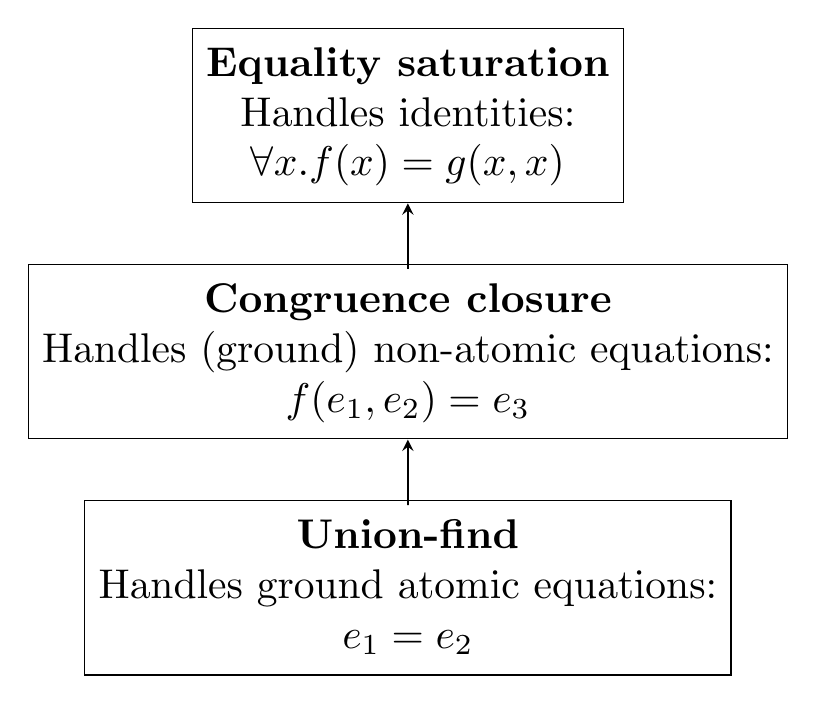
\begin{tikzpicture}[
			scale=1.5,
			transform shape,
			every node/.style={
					draw,
					text height=1.5ex, % Height above the baseline
					text depth=0.25ex,  % Depth below the baseline
					align=center,
					minimum height=3.5\baselineskip
				}
		]
		\node (n0) at (0, 4) {\makecell[c]{\textbf{Equality saturation} \\		
		Handles identities:\\
		$\forall x. f(x) = g(x, x)$}};
		
		\node (n1) at (0, 2) {\makecell[c]{\textbf{Congruence closure} \\		
		Handles (ground) non-atomic equations:\\
		$f(e_1, e_2) = e_3$}};
		
		\node (n2) at (0, 0) {\makecell[c]{\textbf{Union-find} \\
		Handles ground atomic equations:\\
		$e_1 = e_2$}};
		
		\draw[->, >=stealth, thick] (n1.north) to[out=270, in=270] (n0.south);
		
		\draw[->, >=stealth, thick] (n2.north) to[out=270, in=270] (n1.south);
		
	\end{tikzpicture}
\end{figure}

Describing E-graphs can be done in 3 layers. First, there is the union-find structure, which is a simple solver for the theory of atomic equations: given a set of \emph{atoms} $e_1, e_2, \ldots$, we can union two of them to set them equal, and we can find a representative of any particular atom. The representative is unique, so we can simply compare representatives for equality to determine if the atoms they represent are equivalent.

The data structure for this can be thought of as presenting a rewriting system among atoms: for instance,

\begin{align*}
	e_1 &\rightarrow e_1 \\
	e_2 &\rightarrow e_2 \\
	e_3 &\rightarrow e_3 \\
	e_4 &\rightarrow e_4 \\
\end{align*}

is the trivial equivalence relation on 4 atoms. Unioning $e_1$ and $e_2$ gives

\begin{align*}
	e_1 &\rightarrow \underline{e_2} \\
	e_2 &\rightarrow e_2 \\
	e_3 &\rightarrow e_3 \\
	e_4 &\rightarrow e_4 \\
\end{align*}

where we have (arbitrarily) chosen $e_2$ as the new representative.

If we union $e_3$ with $e_4$, we get

\begin{align*}
	e_1 &\rightarrow e_2 \\
	e_2 &\rightarrow e_2 \\
	e_3 &\rightarrow \underline{e_4} \\
	e_4 &\rightarrow e_4 \\
\end{align*}

Now, if we union $e_3$ and $e_2$, we could get

\begin{align*}
	e_1 &\rightarrow e_2 \\
	e_2 &\rightarrow \underline{e_4} \\
	e_3 &\rightarrow e_4 \\
	e_4 &\rightarrow e_4 \\
\end{align*}

Note that we do a lookup before performing the union, so that we union the two \emph{representatives} ($e_4$ of $e_3$ and $e_2$ of $e_2$) together.

Now it takes two steps to rewrite $e_1$ to $e_4$. It is possible to either eagerly canonize the rewrite system on update, setting $e_1$ to rewrite to $e_4$, or do it lazily (compressing such multi-step rewrites on lookup), which is asymptotically more efficient in general. However, these efficiency gains are hard to realize given the congruence closure structure we will build on top of the union-find structure.

On top of union-find, we can build a congruence-closure structure. To handle non-atomic terms, we have to consider function symbols applied to atoms and other terms (like $f(g(e_1), e_2)$), and we need to respect \emph{congruence}: if $s_i = t_i$, then we must conclude $f(s_1, \ldots) = f(t_1, \ldots)$.

To handle congruence, we will break terms down into \emph{layers}. For instance, to represent $f(g(e_1), e_2)$ we will assign a new constant $e_3$ for $g(e_1)$, and then assign a constant $e_4$ for $f(e_3, e_2)$. This way, all congruence checks only need to apply to `flat' terms: if $e_i = d_i$ then we conclude $f(e_1, \ldots) = f(d_1, \ldots)$.

This motivates the E-graph data structure, and the congruence closure algorithm that restores the congruence invariant. Computing the congruence closure is also known as `rebuilding' the E-graph.

\subsection{E-graphs for congruence-closure} \label{egraphs}

As an example, we will compute the congruence closure of the following set of equations:

\begin{align}
  \label{examplecc1}	f(g(a), c) &= h(a, g(b)) \\
  \label{examplecc2}	h(g(c), b) &= h(a, g(c)) \\
  \label{examplecc3}	g(b) &= g(c) \\
  \label{examplecc4}	f(g(a), c) &= g(b)
\end{align}

As a first step, we represent the term $h(a, g(b))$ from \ref{examplecc1}.

\begin{center}
    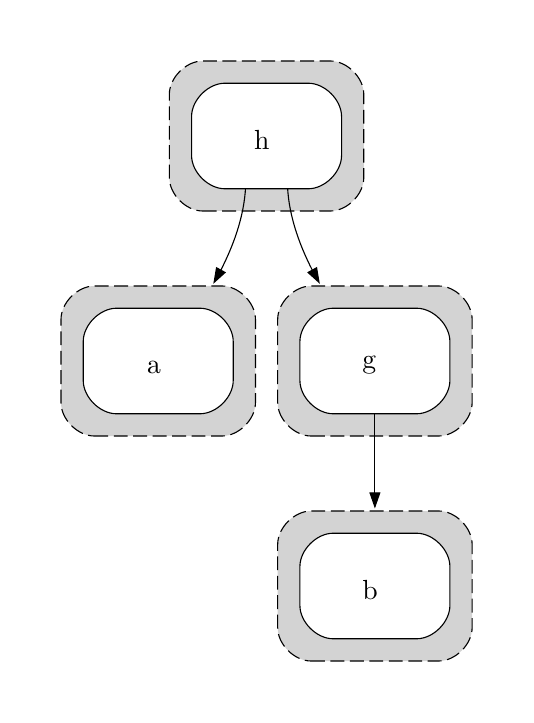
\begin{tikzpicture}[y=1cm, x=1cm, yscale=\globalscale,xscale=\globalscale, every node/.append style={scale=\globalscale}, inner sep=0pt, outer sep=0pt]
  \begin{scope}[shift={(0.1411, -8.3256)}]
    \path[fill=white] (-0.1411, 8.3256) -- (-0.1411, 16.7922) -- (5.9267, 16.7922) -- (5.9267, 8.3256) -- (-0.1411, 8.3256) -- (-0.1411, 8.3256)-- cycle;;



    \path[draw=black,fill=lightgrey,dash pattern=on 0.1764cm off 0.0706cm] (0.7056, 11.6064).. controls (0.7056, 11.6064) and (2.3283, 11.6064) .. (2.3283, 11.6064).. controls (2.54, 11.6064) and (2.7517, 11.8181) .. (2.7517, 12.0297).. controls (2.7517, 12.0297) and (2.7517, 13.0881) .. (2.7517, 13.0881).. controls (2.7517, 13.2997) and (2.54, 13.5114) .. (2.3283, 13.5114).. controls (2.3283, 13.5114) and (0.7056, 13.5114) .. (0.7056, 13.5114).. controls (0.4939, 13.5114) and (0.2822, 13.2997) .. (0.2822, 13.0881).. controls (0.2822, 13.0881) and (0.2822, 12.0297) .. (0.2822, 12.0297).. controls (0.2822, 11.8181) and (0.4939, 11.6064) .. (0.7056, 11.6064);



    \path[draw=black,fill=lightgrey,dash pattern=on 0.1764cm off 0.0706cm] (3.4572, 8.7489).. controls (3.4572, 8.7489) and (5.08, 8.7489) .. (5.08, 8.7489).. controls (5.2917, 8.7489) and (5.5033, 8.9606) .. (5.5033, 9.1722).. controls (5.5033, 9.1722) and (5.5033, 10.2306) .. (5.5033, 10.2306).. controls (5.5033, 10.4422) and (5.2917, 10.6539) .. (5.08, 10.6539).. controls (5.08, 10.6539) and (3.4572, 10.6539) .. (3.4572, 10.6539).. controls (3.2456, 10.6539) and (3.0339, 10.4422) .. (3.0339, 10.2306).. controls (3.0339, 10.2306) and (3.0339, 9.1722) .. (3.0339, 9.1722).. controls (3.0339, 8.9606) and (3.2456, 8.7489) .. (3.4572, 8.7489);



    \path[draw=black,fill=lightgrey,dash pattern=on 0.1764cm off 0.0706cm] (3.4572, 11.6064).. controls (3.4572, 11.6064) and (5.08, 11.6064) .. (5.08, 11.6064).. controls (5.2917, 11.6064) and (5.5033, 11.8181) .. (5.5033, 12.0297).. controls (5.5033, 12.0297) and (5.5033, 13.0881) .. (5.5033, 13.0881).. controls (5.5033, 13.2997) and (5.2917, 13.5114) .. (5.08, 13.5114).. controls (5.08, 13.5114) and (3.4572, 13.5114) .. (3.4572, 13.5114).. controls (3.2456, 13.5114) and (3.0339, 13.2997) .. (3.0339, 13.0881).. controls (3.0339, 13.0881) and (3.0339, 12.0297) .. (3.0339, 12.0297).. controls (3.0339, 11.8181) and (3.2456, 11.6064) .. (3.4572, 11.6064);



    \path[draw=black,fill=lightgrey,dash pattern=on 0.1764cm off 0.0706cm] (2.0814, 14.4639).. controls (2.0814, 14.4639) and (3.7042, 14.4639) .. (3.7042, 14.4639).. controls (3.9158, 14.4639) and (4.1275, 14.6756) .. (4.1275, 14.8872).. controls (4.1275, 14.8872) and (4.1275, 15.9456) .. (4.1275, 15.9456).. controls (4.1275, 16.1572) and (3.9158, 16.3689) .. (3.7042, 16.3689).. controls (3.7042, 16.3689) and (2.0814, 16.3689) .. (2.0814, 16.3689).. controls (1.8697, 16.3689) and (1.6581, 16.1572) .. (1.6581, 15.9456).. controls (1.6581, 15.9456) and (1.6581, 14.8872) .. (1.6581, 14.8872).. controls (1.6581, 14.6756) and (1.8697, 14.4639) .. (2.0814, 14.4639);



    \path[draw=black] (4.2686, 11.9944).. controls (4.2686, 11.6325) and (4.2686, 11.2384) .. (4.2686, 10.8818);



    \path[draw=black,fill=black] (4.3303, 10.8835) -- (4.2686, 10.7072) -- (4.2069, 10.8835) -- (4.3303, 10.8835) -- (4.3303, 10.8835)-- cycle;;



    \path[draw=black] (2.6282, 14.8519).. controls (2.6282, 14.4572) and (2.4899, 14.0596) .. (2.3107, 13.7107);



    \path[draw=black,fill=black] (2.3657, 13.6832) -- (2.2267, 13.558) -- (2.2574, 13.7425) -- (2.3657, 13.6832) -- (2.3657, 13.6832)-- cycle;;



    \path[draw=black] (3.1574, 14.8519).. controls (3.1574, 14.4572) and (3.2957, 14.0596) .. (3.4749, 13.7107);



    \path[draw=black,fill=black] (3.5281, 13.7425) -- (3.5588, 13.558) -- (3.4198, 13.6832) -- (3.5281, 13.7425) -- (3.5281, 13.7425)-- cycle;;



    \path[draw=black,fill=white] (2.0461, 13.2292).. controls (2.0461, 13.2292) and (0.9878, 13.2292) .. (0.9878, 13.2292).. controls (0.7761, 13.2292) and (0.5644, 13.0175) .. (0.5644, 12.8058).. controls (0.5644, 12.8058) and (0.5644, 12.3119) .. (0.5644, 12.3119).. controls (0.5644, 12.1003) and (0.7761, 11.8886) .. (0.9878, 11.8886).. controls (0.9878, 11.8886) and (2.0461, 11.8886) .. (2.0461, 11.8886).. controls (2.2578, 11.8886) and (2.4694, 12.1003) .. (2.4694, 12.3119).. controls (2.4694, 12.3119) and (2.4694, 12.8058) .. (2.4694, 12.8058).. controls (2.4694, 13.0175) and (2.2578, 13.2292) .. (2.0461, 13.2292);



    \node[anchor=south west] (text3495) at (1.3716, 12.3941){a};



    \path[draw=black,fill=white] (4.7978, 10.3717).. controls (4.7978, 10.3717) and (3.7394, 10.3717) .. (3.7394, 10.3717).. controls (3.5278, 10.3717) and (3.3161, 10.16) .. (3.3161, 9.9483).. controls (3.3161, 9.9483) and (3.3161, 9.4544) .. (3.3161, 9.4544).. controls (3.3161, 9.2428) and (3.5278, 9.0311) .. (3.7394, 9.0311).. controls (3.7394, 9.0311) and (4.7978, 9.0311) .. (4.7978, 9.0311).. controls (5.0094, 9.0311) and (5.2211, 9.2428) .. (5.2211, 9.4544).. controls (5.2211, 9.4544) and (5.2211, 9.9483) .. (5.2211, 9.9483).. controls (5.2211, 10.16) and (5.0094, 10.3717) .. (4.7978, 10.3717);



    \node[anchor=south west] (text4176) at (4.1099, 9.5363){b};



    \path[draw=black,fill=white] (4.7978, 13.2292).. controls (4.7978, 13.2292) and (3.7394, 13.2292) .. (3.7394, 13.2292).. controls (3.5278, 13.2292) and (3.3161, 13.0175) .. (3.3161, 12.8058).. controls (3.3161, 12.8058) and (3.3161, 12.3119) .. (3.3161, 12.3119).. controls (3.3161, 12.1003) and (3.5278, 11.8886) .. (3.7394, 11.8886).. controls (3.7394, 11.8886) and (4.7978, 11.8886) .. (4.7978, 11.8886).. controls (5.0094, 11.8886) and (5.2211, 12.1003) .. (5.2211, 12.3119).. controls (5.2211, 12.3119) and (5.2211, 12.8058) .. (5.2211, 12.8058).. controls (5.2211, 13.0175) and (5.0094, 13.2292) .. (4.7978, 13.2292);



    \node[anchor=south west] (text9304) at (4.1099, 12.3941){g};



    \path[draw=black,fill=white] (3.4219, 16.0867).. controls (3.4219, 16.0867) and (2.3636, 16.0867) .. (2.3636, 16.0867).. controls (2.1519, 16.0867) and (1.9403, 15.875) .. (1.9403, 15.6633).. controls (1.9403, 15.6633) and (1.9403, 15.1694) .. (1.9403, 15.1694).. controls (1.9403, 14.9578) and (2.1519, 14.7461) .. (2.3636, 14.7461).. controls (2.3636, 14.7461) and (3.4219, 14.7461) .. (3.4219, 14.7461).. controls (3.6336, 14.7461) and (3.8453, 14.9578) .. (3.8453, 15.1694).. controls (3.8453, 15.1694) and (3.8453, 15.6633) .. (3.8453, 15.6633).. controls (3.8453, 15.875) and (3.6336, 16.0867) .. (3.4219, 16.0867);



    \node[anchor=south west] (text8938) at (2.734, 15.2513){h};



  \end{scope}

\end{tikzpicture}
    \label{exampleBasic1}
\end{center}

Notice how we have flattened the term: the three levels of nesting become pointers between the three layers of our graph.

Then we will add the other term $f(g(a), c)$ from \ref{examplecc1}.

\begin{center}
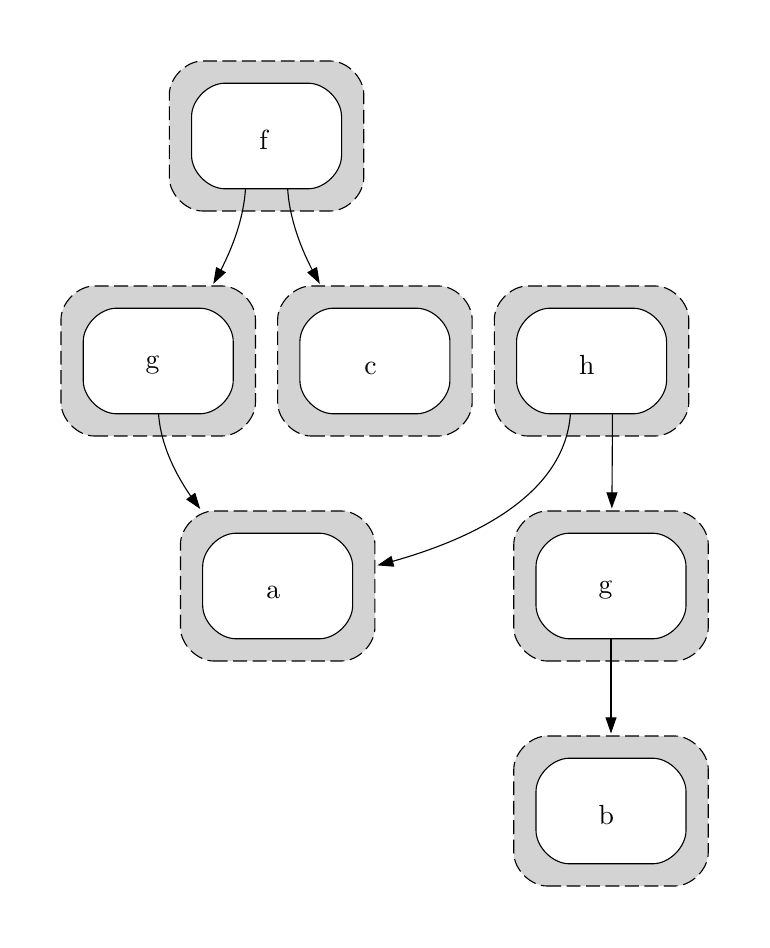
\begin{tikzpicture}[y=1cm, x=1cm, yscale=\globalscale,xscale=\globalscale, every node/.append style={scale=\globalscale}, inner sep=0pt, outer sep=0pt]
  \begin{scope}[shift={(0.1411, -11.1831)}]
    \path[fill=white] (-0.1411, 11.1831) -- (-0.1411, 22.5072) -- (8.9253, 22.5072) -- (8.9253, 11.1831) -- (-0.1411, 11.1831) -- (-0.1411, 11.1831)-- cycle;;



    \path[draw=black,fill=lightgrey,dash pattern=on 0.1764cm off 0.0706cm] (2.2225, 14.4639).. controls (2.2225, 14.4639) and (3.8453, 14.4639) .. (3.8453, 14.4639).. controls (4.0569, 14.4639) and (4.2686, 14.6756) .. (4.2686, 14.8872).. controls (4.2686, 14.8872) and (4.2686, 15.9456) .. (4.2686, 15.9456).. controls (4.2686, 16.1572) and (4.0569, 16.3689) .. (3.8453, 16.3689).. controls (3.8453, 16.3689) and (2.2225, 16.3689) .. (2.2225, 16.3689).. controls (2.0108, 16.3689) and (1.7992, 16.1572) .. (1.7992, 15.9456).. controls (1.7992, 15.9456) and (1.7992, 14.8872) .. (1.7992, 14.8872).. controls (1.7992, 14.6756) and (2.0108, 14.4639) .. (2.2225, 14.4639);



    \path[draw=black,fill=lightgrey,dash pattern=on 0.1764cm off 0.0706cm] (0.7056, 17.3214).. controls (0.7056, 17.3214) and (2.3283, 17.3214) .. (2.3283, 17.3214).. controls (2.54, 17.3214) and (2.7517, 17.5331) .. (2.7517, 17.7447).. controls (2.7517, 17.7447) and (2.7517, 18.8031) .. (2.7517, 18.8031).. controls (2.7517, 19.0147) and (2.54, 19.2264) .. (2.3283, 19.2264).. controls (2.3283, 19.2264) and (0.7056, 19.2264) .. (0.7056, 19.2264).. controls (0.4939, 19.2264) and (0.2822, 19.0147) .. (0.2822, 18.8031).. controls (0.2822, 18.8031) and (0.2822, 17.7447) .. (0.2822, 17.7447).. controls (0.2822, 17.5331) and (0.4939, 17.3214) .. (0.7056, 17.3214);



    \path[draw=black,fill=lightgrey,dash pattern=on 0.1764cm off 0.0706cm] (3.4572, 17.3214).. controls (3.4572, 17.3214) and (5.08, 17.3214) .. (5.08, 17.3214).. controls (5.2917, 17.3214) and (5.5033, 17.5331) .. (5.5033, 17.7447).. controls (5.5033, 17.7447) and (5.5033, 18.8031) .. (5.5033, 18.8031).. controls (5.5033, 19.0147) and (5.2917, 19.2264) .. (5.08, 19.2264).. controls (5.08, 19.2264) and (3.4572, 19.2264) .. (3.4572, 19.2264).. controls (3.2456, 19.2264) and (3.0339, 19.0147) .. (3.0339, 18.8031).. controls (3.0339, 18.8031) and (3.0339, 17.7447) .. (3.0339, 17.7447).. controls (3.0339, 17.5331) and (3.2456, 17.3214) .. (3.4572, 17.3214);



    \path[draw=black,fill=lightgrey,dash pattern=on 0.1764cm off 0.0706cm] (2.0814, 20.1789).. controls (2.0814, 20.1789) and (3.7042, 20.1789) .. (3.7042, 20.1789).. controls (3.9158, 20.1789) and (4.1275, 20.3906) .. (4.1275, 20.6022).. controls (4.1275, 20.6022) and (4.1275, 21.6606) .. (4.1275, 21.6606).. controls (4.1275, 21.8722) and (3.9158, 22.0839) .. (3.7042, 22.0839).. controls (3.7042, 22.0839) and (2.0814, 22.0839) .. (2.0814, 22.0839).. controls (1.8697, 22.0839) and (1.6581, 21.8722) .. (1.6581, 21.6606).. controls (1.6581, 21.6606) and (1.6581, 20.6022) .. (1.6581, 20.6022).. controls (1.6581, 20.3906) and (1.8697, 20.1789) .. (2.0814, 20.1789);



    \path[draw=black,fill=lightgrey,dash pattern=on 0.1764cm off 0.0706cm] (6.4558, 11.6064).. controls (6.4558, 11.6064) and (8.0786, 11.6064) .. (8.0786, 11.6064).. controls (8.2903, 11.6064) and (8.5019, 11.8181) .. (8.5019, 12.0297).. controls (8.5019, 12.0297) and (8.5019, 13.0881) .. (8.5019, 13.0881).. controls (8.5019, 13.2997) and (8.2903, 13.5114) .. (8.0786, 13.5114).. controls (8.0786, 13.5114) and (6.4558, 13.5114) .. (6.4558, 13.5114).. controls (6.2442, 13.5114) and (6.0325, 13.2997) .. (6.0325, 13.0881).. controls (6.0325, 13.0881) and (6.0325, 12.0297) .. (6.0325, 12.0297).. controls (6.0325, 11.8181) and (6.2442, 11.6064) .. (6.4558, 11.6064);



    \path[draw=black,fill=lightgrey,dash pattern=on 0.1764cm off 0.0706cm] (6.4558, 14.4639).. controls (6.4558, 14.4639) and (8.0786, 14.4639) .. (8.0786, 14.4639).. controls (8.2903, 14.4639) and (8.5019, 14.6756) .. (8.5019, 14.8872).. controls (8.5019, 14.8872) and (8.5019, 15.9456) .. (8.5019, 15.9456).. controls (8.5019, 16.1572) and (8.2903, 16.3689) .. (8.0786, 16.3689).. controls (8.0786, 16.3689) and (6.4558, 16.3689) .. (6.4558, 16.3689).. controls (6.2442, 16.3689) and (6.0325, 16.1572) .. (6.0325, 15.9456).. controls (6.0325, 15.9456) and (6.0325, 14.8872) .. (6.0325, 14.8872).. controls (6.0325, 14.6756) and (6.2442, 14.4639) .. (6.4558, 14.4639);



    \path[draw=black,fill=lightgrey,dash pattern=on 0.1764cm off 0.0706cm] (6.2089, 17.3214).. controls (6.2089, 17.3214) and (7.8317, 17.3214) .. (7.8317, 17.3214).. controls (8.0433, 17.3214) and (8.255, 17.5331) .. (8.255, 17.7447).. controls (8.255, 17.7447) and (8.255, 18.8031) .. (8.255, 18.8031).. controls (8.255, 19.0147) and (8.0433, 19.2264) .. (7.8317, 19.2264).. controls (7.8317, 19.2264) and (6.2089, 19.2264) .. (6.2089, 19.2264).. controls (5.9972, 19.2264) and (5.7856, 19.0147) .. (5.7856, 18.8031).. controls (5.7856, 18.8031) and (5.7856, 17.7447) .. (5.7856, 17.7447).. controls (5.7856, 17.5331) and (5.9972, 17.3214) .. (6.2089, 17.3214);



    \path[draw=black] (1.5169, 17.7094).. controls (1.5169, 17.2928) and (1.6972, 16.8952) .. (1.9332, 16.553);



    \path[draw=black,fill=black] (1.9826, 16.5901) -- (2.0376, 16.4116) -- (1.8831, 16.5167) -- (1.9826, 16.5901) -- (1.9826, 16.5901)-- cycle;;



    \path[draw=black] (2.6282, 20.5669).. controls (2.6282, 20.1722) and (2.4899, 19.7746) .. (2.3107, 19.4257);



    \path[draw=black,fill=black] (2.3657, 19.3982) -- (2.2267, 19.273) -- (2.2574, 19.4575) -- (2.3657, 19.3982) -- (2.3657, 19.3982)-- cycle;;



    \path[draw=black] (3.1574, 20.5669).. controls (3.1574, 20.1722) and (3.2957, 19.7746) .. (3.4749, 19.4257);



    \path[draw=black,fill=black] (3.5281, 19.4575) -- (3.5588, 19.273) -- (3.4198, 19.3982) -- (3.5281, 19.4575) -- (3.5281, 19.4575)-- cycle;;



    \path[draw=black] (7.2672, 14.8519).. controls (7.2672, 14.49) and (7.2672, 14.0959) .. (7.2672, 13.7393);



    \path[draw=black,fill=black] (7.329, 13.741) -- (7.2672, 13.5647) -- (7.2055, 13.741) -- (7.329, 13.741) -- (7.329, 13.741)-- cycle;;



    \path[draw=black] (6.7557, 17.7094).. controls (6.7557, 16.6) and (5.5319, 16.0207) .. (4.488, 15.7282);



    \path[draw=black,fill=black] (4.5064, 15.669) -- (4.3201, 15.6838) -- (4.4746, 15.7886) -- (4.5064, 15.669) -- (4.5064, 15.669)-- cycle;;



    \path[draw=black] (7.2849, 17.7094).. controls (7.2849, 17.3475) and (7.2827, 16.9531) .. (7.2796, 16.5968);



    \path[draw=black,fill=black] (7.3413, 16.5978) -- (7.2782, 16.4222) -- (7.2178, 16.5989) -- (7.3413, 16.5978) -- (7.3413, 16.5978)-- cycle;;



    \path[draw=black,fill=white] (3.5631, 16.0867).. controls (3.5631, 16.0867) and (2.5047, 16.0867) .. (2.5047, 16.0867).. controls (2.2931, 16.0867) and (2.0814, 15.875) .. (2.0814, 15.6633).. controls (2.0814, 15.6633) and (2.0814, 15.1694) .. (2.0814, 15.1694).. controls (2.0814, 14.9578) and (2.2931, 14.7461) .. (2.5047, 14.7461).. controls (2.5047, 14.7461) and (3.5631, 14.7461) .. (3.5631, 14.7461).. controls (3.7747, 14.7461) and (3.9864, 14.9578) .. (3.9864, 15.1694).. controls (3.9864, 15.1694) and (3.9864, 15.6633) .. (3.9864, 15.6633).. controls (3.9864, 15.875) and (3.7747, 16.0867) .. (3.5631, 16.0867);



    \node[anchor=south west] (text4956) at (2.8885, 15.2516){a};



    \path[draw=black,fill=white] (2.0461, 18.9442).. controls (2.0461, 18.9442) and (0.9878, 18.9442) .. (0.9878, 18.9442).. controls (0.7761, 18.9442) and (0.5644, 18.7325) .. (0.5644, 18.5208).. controls (0.5644, 18.5208) and (0.5644, 18.0269) .. (0.5644, 18.0269).. controls (0.5644, 17.8153) and (0.7761, 17.6036) .. (0.9878, 17.6036).. controls (0.9878, 17.6036) and (2.0461, 17.6036) .. (2.0461, 17.6036).. controls (2.2578, 17.6036) and (2.4694, 17.8153) .. (2.4694, 18.0269).. controls (2.4694, 18.0269) and (2.4694, 18.5208) .. (2.4694, 18.5208).. controls (2.4694, 18.7325) and (2.2578, 18.9442) .. (2.0461, 18.9442);



    \node[anchor=south west] (text6317) at (1.3582, 18.1088){g};



    \path[draw=black,fill=white] (4.7978, 18.9442).. controls (4.7978, 18.9442) and (3.7394, 18.9442) .. (3.7394, 18.9442).. controls (3.5278, 18.9442) and (3.3161, 18.7325) .. (3.3161, 18.5208).. controls (3.3161, 18.5208) and (3.3161, 18.0269) .. (3.3161, 18.0269).. controls (3.3161, 17.8153) and (3.5278, 17.6036) .. (3.7394, 17.6036).. controls (3.7394, 17.6036) and (4.7978, 17.6036) .. (4.7978, 17.6036).. controls (5.0094, 17.6036) and (5.2211, 17.8153) .. (5.2211, 18.0269).. controls (5.2211, 18.0269) and (5.2211, 18.5208) .. (5.2211, 18.5208).. controls (5.2211, 18.7325) and (5.0094, 18.9442) .. (4.7978, 18.9442);



    \node[anchor=south west] (text9774) at (4.1363, 18.1088){c};



    \path[draw=black,fill=white] (3.4219, 21.8017).. controls (3.4219, 21.8017) and (2.3636, 21.8017) .. (2.3636, 21.8017).. controls (2.1519, 21.8017) and (1.9403, 21.59) .. (1.9403, 21.3783).. controls (1.9403, 21.3783) and (1.9403, 20.8844) .. (1.9403, 20.8844).. controls (1.9403, 20.6728) and (2.1519, 20.4611) .. (2.3636, 20.4611).. controls (2.3636, 20.4611) and (3.4219, 20.4611) .. (3.4219, 20.4611).. controls (3.6336, 20.4611) and (3.8453, 20.6728) .. (3.8453, 20.8844).. controls (3.8453, 20.8844) and (3.8453, 21.3783) .. (3.8453, 21.3783).. controls (3.8453, 21.59) and (3.6336, 21.8017) .. (3.4219, 21.8017);



    \node[anchor=south west] (text345) at (2.8003, 20.9663){f};



    \path[draw=black,fill=white] (7.7964, 13.2292).. controls (7.7964, 13.2292) and (6.7381, 13.2292) .. (6.7381, 13.2292).. controls (6.5264, 13.2292) and (6.3147, 13.0175) .. (6.3147, 12.8058).. controls (6.3147, 12.8058) and (6.3147, 12.3119) .. (6.3147, 12.3119).. controls (6.3147, 12.1003) and (6.5264, 11.8886) .. (6.7381, 11.8886).. controls (6.7381, 11.8886) and (7.7964, 11.8886) .. (7.7964, 11.8886).. controls (8.0081, 11.8886) and (8.2197, 12.1003) .. (8.2197, 12.3119).. controls (8.2197, 12.3119) and (8.2197, 12.8058) .. (8.2197, 12.8058).. controls (8.2197, 13.0175) and (8.0081, 13.2292) .. (7.7964, 13.2292);



    \node[anchor=south west] (text2776) at (7.1085, 12.3938){b};



    \path[draw=black,fill=white] (7.7964, 16.0867).. controls (7.7964, 16.0867) and (6.7381, 16.0867) .. (6.7381, 16.0867).. controls (6.5264, 16.0867) and (6.3147, 15.875) .. (6.3147, 15.6633).. controls (6.3147, 15.6633) and (6.3147, 15.1694) .. (6.3147, 15.1694).. controls (6.3147, 14.9578) and (6.5264, 14.7461) .. (6.7381, 14.7461).. controls (6.7381, 14.7461) and (7.7964, 14.7461) .. (7.7964, 14.7461).. controls (8.0081, 14.7461) and (8.2197, 14.9578) .. (8.2197, 15.1694).. controls (8.2197, 15.1694) and (8.2197, 15.6633) .. (8.2197, 15.6633).. controls (8.2197, 15.875) and (8.0081, 16.0867) .. (7.7964, 16.0867);



    \node[anchor=south west] (text1316) at (7.1085, 15.2516){g};



    \path[draw=black,fill=white] (7.5494, 18.9442).. controls (7.5494, 18.9442) and (6.4911, 18.9442) .. (6.4911, 18.9442).. controls (6.2794, 18.9442) and (6.0678, 18.7325) .. (6.0678, 18.5208).. controls (6.0678, 18.5208) and (6.0678, 18.0269) .. (6.0678, 18.0269).. controls (6.0678, 17.8153) and (6.2794, 17.6036) .. (6.4911, 17.6036).. controls (6.4911, 17.6036) and (7.5494, 17.6036) .. (7.5494, 17.6036).. controls (7.7611, 17.6036) and (7.9728, 17.8153) .. (7.9728, 18.0269).. controls (7.9728, 18.0269) and (7.9728, 18.5208) .. (7.9728, 18.5208).. controls (7.9728, 18.7325) and (7.7611, 18.9442) .. (7.5494, 18.9442);



    \node[anchor=south west] (text4476) at (6.8615, 18.1088){h};



  \end{scope}

\end{tikzpicture}
    \label{exampleBasic2}
\end{center}

Now, as a final step, we need to \emph{union} the two top nodes of both sides of the equation:

\begin{center}
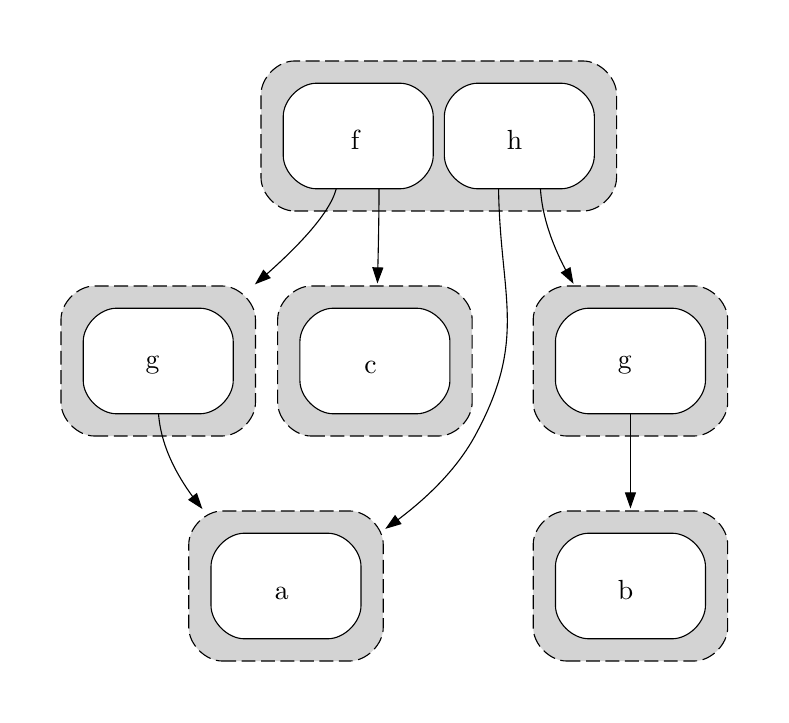
\begin{tikzpicture}[y=1cm, x=1cm, yscale=\globalscale,xscale=\globalscale, every node/.append style={scale=\globalscale}, inner sep=0pt, outer sep=0pt]
  \begin{scope}[shift={(0.1411, -8.3256)}]
    \path[fill=white] (-0.1411, 8.3256) -- (-0.1411, 16.7922) -- (9.1722, 16.7922) -- (9.1722, 8.3256) -- (-0.1411, 8.3256) -- (-0.1411, 8.3256)-- cycle;;



    \path[draw=black,fill=lightgrey,dash pattern=on 0.1764cm off 0.0706cm] (2.3283, 8.7489).. controls (2.3283, 8.7489) and (3.9511, 8.7489) .. (3.9511, 8.7489).. controls (4.1628, 8.7489) and (4.3744, 8.9606) .. (4.3744, 9.1722).. controls (4.3744, 9.1722) and (4.3744, 10.2306) .. (4.3744, 10.2306).. controls (4.3744, 10.4422) and (4.1628, 10.6539) .. (3.9511, 10.6539).. controls (3.9511, 10.6539) and (2.3283, 10.6539) .. (2.3283, 10.6539).. controls (2.1167, 10.6539) and (1.905, 10.4422) .. (1.905, 10.2306).. controls (1.905, 10.2306) and (1.905, 9.1722) .. (1.905, 9.1722).. controls (1.905, 8.9606) and (2.1167, 8.7489) .. (2.3283, 8.7489);



    \path[draw=black,fill=lightgrey,dash pattern=on 0.1764cm off 0.0706cm] (0.7056, 11.6064).. controls (0.7056, 11.6064) and (2.3283, 11.6064) .. (2.3283, 11.6064).. controls (2.54, 11.6064) and (2.7517, 11.8181) .. (2.7517, 12.0297).. controls (2.7517, 12.0297) and (2.7517, 13.0881) .. (2.7517, 13.0881).. controls (2.7517, 13.2997) and (2.54, 13.5114) .. (2.3283, 13.5114).. controls (2.3283, 13.5114) and (0.7056, 13.5114) .. (0.7056, 13.5114).. controls (0.4939, 13.5114) and (0.2822, 13.2997) .. (0.2822, 13.0881).. controls (0.2822, 13.0881) and (0.2822, 12.0297) .. (0.2822, 12.0297).. controls (0.2822, 11.8181) and (0.4939, 11.6064) .. (0.7056, 11.6064);



    \path[draw=black,fill=lightgrey,dash pattern=on 0.1764cm off 0.0706cm] (3.4572, 11.6064).. controls (3.4572, 11.6064) and (5.08, 11.6064) .. (5.08, 11.6064).. controls (5.2917, 11.6064) and (5.5033, 11.8181) .. (5.5033, 12.0297).. controls (5.5033, 12.0297) and (5.5033, 13.0881) .. (5.5033, 13.0881).. controls (5.5033, 13.2997) and (5.2917, 13.5114) .. (5.08, 13.5114).. controls (5.08, 13.5114) and (3.4572, 13.5114) .. (3.4572, 13.5114).. controls (3.2456, 13.5114) and (3.0339, 13.2997) .. (3.0339, 13.0881).. controls (3.0339, 13.0881) and (3.0339, 12.0297) .. (3.0339, 12.0297).. controls (3.0339, 11.8181) and (3.2456, 11.6064) .. (3.4572, 11.6064);



    \path[draw=black,fill=lightgrey,dash pattern=on 0.1764cm off 0.0706cm] (3.2456, 14.4639).. controls (3.2456, 14.4639) and (6.9144, 14.4639) .. (6.9144, 14.4639).. controls (7.1261, 14.4639) and (7.3378, 14.6756) .. (7.3378, 14.8872).. controls (7.3378, 14.8872) and (7.3378, 15.9456) .. (7.3378, 15.9456).. controls (7.3378, 16.1572) and (7.1261, 16.3689) .. (6.9144, 16.3689).. controls (6.9144, 16.3689) and (3.2456, 16.3689) .. (3.2456, 16.3689).. controls (3.0339, 16.3689) and (2.8222, 16.1572) .. (2.8222, 15.9456).. controls (2.8222, 15.9456) and (2.8222, 14.8872) .. (2.8222, 14.8872).. controls (2.8222, 14.6756) and (3.0339, 14.4639) .. (3.2456, 14.4639);



    \path[draw=black,fill=lightgrey,dash pattern=on 0.1764cm off 0.0706cm] (6.7028, 8.7489).. controls (6.7028, 8.7489) and (8.3256, 8.7489) .. (8.3256, 8.7489).. controls (8.5372, 8.7489) and (8.7489, 8.9606) .. (8.7489, 9.1722).. controls (8.7489, 9.1722) and (8.7489, 10.2306) .. (8.7489, 10.2306).. controls (8.7489, 10.4422) and (8.5372, 10.6539) .. (8.3256, 10.6539).. controls (8.3256, 10.6539) and (6.7028, 10.6539) .. (6.7028, 10.6539).. controls (6.4911, 10.6539) and (6.2794, 10.4422) .. (6.2794, 10.2306).. controls (6.2794, 10.2306) and (6.2794, 9.1722) .. (6.2794, 9.1722).. controls (6.2794, 8.9606) and (6.4911, 8.7489) .. (6.7028, 8.7489);



    \path[draw=black,fill=lightgrey,dash pattern=on 0.1764cm off 0.0706cm] (6.7028, 11.6064).. controls (6.7028, 11.6064) and (8.3256, 11.6064) .. (8.3256, 11.6064).. controls (8.5372, 11.6064) and (8.7489, 11.8181) .. (8.7489, 12.0297).. controls (8.7489, 12.0297) and (8.7489, 13.0881) .. (8.7489, 13.0881).. controls (8.7489, 13.2997) and (8.5372, 13.5114) .. (8.3256, 13.5114).. controls (8.3256, 13.5114) and (6.7028, 13.5114) .. (6.7028, 13.5114).. controls (6.4911, 13.5114) and (6.2794, 13.2997) .. (6.2794, 13.0881).. controls (6.2794, 13.0881) and (6.2794, 12.0297) .. (6.2794, 12.0297).. controls (6.2794, 11.8181) and (6.4911, 11.6064) .. (6.7028, 11.6064);



    \path[draw=black] (1.5169, 11.9944).. controls (1.5169, 11.569) and (1.7092, 11.1689) .. (1.9614, 10.8271);



    \path[draw=black,fill=black] (2.0045, 10.8726) -- (2.0652, 10.6959) -- (1.9075, 10.7961) -- (2.0045, 10.8726) -- (2.0045, 10.8726)-- cycle;;



    \path[draw=black] (3.7924, 14.8519).. controls (3.7924, 14.5443) and (3.368, 14.0811) .. (2.8857, 13.6543);



    \path[draw=black,fill=black] (2.9348, 13.6151) -- (2.7608, 13.5463) -- (2.8536, 13.7086) -- (2.9348, 13.6151) -- (2.9348, 13.6151)-- cycle;;



    \path[draw=black] (4.3215, 14.8519).. controls (4.3215, 14.49) and (4.3148, 14.0956) .. (4.306, 13.7393);



    \path[draw=black,fill=black] (4.3677, 13.7393) -- (4.3014, 13.5647) -- (4.2443, 13.7428) -- (4.3677, 13.7393) -- (4.3677, 13.7393)-- cycle;;



    \path[draw=black] (5.8385, 14.8519).. controls (5.8385, 13.4034) and (6.2336, 12.8774) .. (5.5386, 11.6064).. controls (5.3068, 11.1823) and (4.934, 10.8225) .. (4.5508, 10.5354);



    \path[draw=black,fill=black] (4.597, 10.4923) -- (4.4178, 10.4394) -- (4.5247, 10.5925) -- (4.597, 10.4923) -- (4.597, 10.4923)-- cycle;;



    \path[draw=black] (6.3676, 14.8519).. controls (6.3676, 14.4558) and (6.5098, 14.0585) .. (6.694, 13.7104);



    \path[draw=black,fill=black] (6.7472, 13.7418) -- (6.7804, 13.5576) -- (6.6396, 13.6807) -- (6.7472, 13.7418) -- (6.7472, 13.7418)-- cycle;;



    \path[draw=black] (7.5142, 11.9944).. controls (7.5142, 11.6325) and (7.5142, 11.2384) .. (7.5142, 10.8818);



    \path[draw=black,fill=black] (7.5759, 10.8835) -- (7.5142, 10.7072) -- (7.4524, 10.8835) -- (7.5759, 10.8835) -- (7.5759, 10.8835)-- cycle;;



    \path[draw=black,fill=white] (3.6689, 10.3717).. controls (3.6689, 10.3717) and (2.6106, 10.3717) .. (2.6106, 10.3717).. controls (2.3989, 10.3717) and (2.1872, 10.16) .. (2.1872, 9.9483).. controls (2.1872, 9.9483) and (2.1872, 9.4544) .. (2.1872, 9.4544).. controls (2.1872, 9.2428) and (2.3989, 9.0311) .. (2.6106, 9.0311).. controls (2.6106, 9.0311) and (3.6689, 9.0311) .. (3.6689, 9.0311).. controls (3.8806, 9.0311) and (4.0922, 9.2428) .. (4.0922, 9.4544).. controls (4.0922, 9.4544) and (4.0922, 9.9483) .. (4.0922, 9.9483).. controls (4.0922, 10.16) and (3.8806, 10.3717) .. (3.6689, 10.3717);



    \node[anchor=south west] (text2534) at (2.9944, 9.5363){a};



    \path[draw=black,fill=white] (2.0461, 13.2292).. controls (2.0461, 13.2292) and (0.9878, 13.2292) .. (0.9878, 13.2292).. controls (0.7761, 13.2292) and (0.5644, 13.0175) .. (0.5644, 12.8058).. controls (0.5644, 12.8058) and (0.5644, 12.3119) .. (0.5644, 12.3119).. controls (0.5644, 12.1003) and (0.7761, 11.8886) .. (0.9878, 11.8886).. controls (0.9878, 11.8886) and (2.0461, 11.8886) .. (2.0461, 11.8886).. controls (2.2578, 11.8886) and (2.4694, 12.1003) .. (2.4694, 12.3119).. controls (2.4694, 12.3119) and (2.4694, 12.8058) .. (2.4694, 12.8058).. controls (2.4694, 13.0175) and (2.2578, 13.2292) .. (2.0461, 13.2292);



    \node[anchor=south west] (text1917) at (1.3582, 12.3941){g};



    \path[draw=black,fill=white] (4.7978, 13.2292).. controls (4.7978, 13.2292) and (3.7394, 13.2292) .. (3.7394, 13.2292).. controls (3.5278, 13.2292) and (3.3161, 13.0175) .. (3.3161, 12.8058).. controls (3.3161, 12.8058) and (3.3161, 12.3119) .. (3.3161, 12.3119).. controls (3.3161, 12.1003) and (3.5278, 11.8886) .. (3.7394, 11.8886).. controls (3.7394, 11.8886) and (4.7978, 11.8886) .. (4.7978, 11.8886).. controls (5.0094, 11.8886) and (5.2211, 12.1003) .. (5.2211, 12.3119).. controls (5.2211, 12.3119) and (5.2211, 12.8058) .. (5.2211, 12.8058).. controls (5.2211, 13.0175) and (5.0094, 13.2292) .. (4.7978, 13.2292);



    \node[anchor=south west] (text9645) at (4.1363, 12.3941){c};



    \path[draw=black,fill=white] (4.5861, 16.0867).. controls (4.5861, 16.0867) and (3.5278, 16.0867) .. (3.5278, 16.0867).. controls (3.3161, 16.0867) and (3.1044, 15.875) .. (3.1044, 15.6633).. controls (3.1044, 15.6633) and (3.1044, 15.1694) .. (3.1044, 15.1694).. controls (3.1044, 14.9578) and (3.3161, 14.7461) .. (3.5278, 14.7461).. controls (3.5278, 14.7461) and (4.5861, 14.7461) .. (4.5861, 14.7461).. controls (4.7978, 14.7461) and (5.0094, 14.9578) .. (5.0094, 15.1694).. controls (5.0094, 15.1694) and (5.0094, 15.6633) .. (5.0094, 15.6633).. controls (5.0094, 15.875) and (4.7978, 16.0867) .. (4.5861, 16.0867);



    \node[anchor=south west] (text9315) at (3.9645, 15.2513){f};



    \path[draw=black,fill=white] (6.6322, 16.0867).. controls (6.6322, 16.0867) and (5.5739, 16.0867) .. (5.5739, 16.0867).. controls (5.3622, 16.0867) and (5.1506, 15.875) .. (5.1506, 15.6633).. controls (5.1506, 15.6633) and (5.1506, 15.1694) .. (5.1506, 15.1694).. controls (5.1506, 14.9578) and (5.3622, 14.7461) .. (5.5739, 14.7461).. controls (5.5739, 14.7461) and (6.6322, 14.7461) .. (6.6322, 14.7461).. controls (6.8439, 14.7461) and (7.0556, 14.9578) .. (7.0556, 15.1694).. controls (7.0556, 15.1694) and (7.0556, 15.6633) .. (7.0556, 15.6633).. controls (7.0556, 15.875) and (6.8439, 16.0867) .. (6.6322, 16.0867);



    \node[anchor=south west] (text9153) at (5.9443, 15.2513){h};



    \path[draw=black,fill=white] (8.0433, 13.2292).. controls (8.0433, 13.2292) and (6.985, 13.2292) .. (6.985, 13.2292).. controls (6.7733, 13.2292) and (6.5617, 13.0175) .. (6.5617, 12.8058).. controls (6.5617, 12.8058) and (6.5617, 12.3119) .. (6.5617, 12.3119).. controls (6.5617, 12.1003) and (6.7733, 11.8886) .. (6.985, 11.8886).. controls (6.985, 11.8886) and (8.0433, 11.8886) .. (8.0433, 11.8886).. controls (8.255, 11.8886) and (8.4667, 12.1003) .. (8.4667, 12.3119).. controls (8.4667, 12.3119) and (8.4667, 12.8058) .. (8.4667, 12.8058).. controls (8.4667, 13.0175) and (8.255, 13.2292) .. (8.0433, 13.2292);



    \node[anchor=south west] (text6846) at (7.3554, 12.3941){g};



    \path[draw=black,fill=white] (8.0433, 10.3717).. controls (8.0433, 10.3717) and (6.985, 10.3717) .. (6.985, 10.3717).. controls (6.7733, 10.3717) and (6.5617, 10.16) .. (6.5617, 9.9483).. controls (6.5617, 9.9483) and (6.5617, 9.4544) .. (6.5617, 9.4544).. controls (6.5617, 9.2428) and (6.7733, 9.0311) .. (6.985, 9.0311).. controls (6.985, 9.0311) and (8.0433, 9.0311) .. (8.0433, 9.0311).. controls (8.255, 9.0311) and (8.4667, 9.2428) .. (8.4667, 9.4544).. controls (8.4667, 9.4544) and (8.4667, 9.9483) .. (8.4667, 9.9483).. controls (8.4667, 10.16) and (8.255, 10.3717) .. (8.0433, 10.3717);



    \node[anchor=south west] (text3608) at (7.3554, 9.5363){b};



  \end{scope}

\end{tikzpicture}
\label{exampleBasic3}
\end{center}

We call the outer nodes \emph{E-classes} (equivalence classes), while the inner nodes are \emph{E-nodes}. E-classes can contain multiple E-nodes. The arrows point from E-nodes to E-classes.

Next we move on to \ref{examplecc2}. This time, notice that the subterm $g(c)$ is used twice, and we \emph{share} this in the E-graph, indicated by two arrows pointing to the E-class for $g(c)$.

\begin{center}
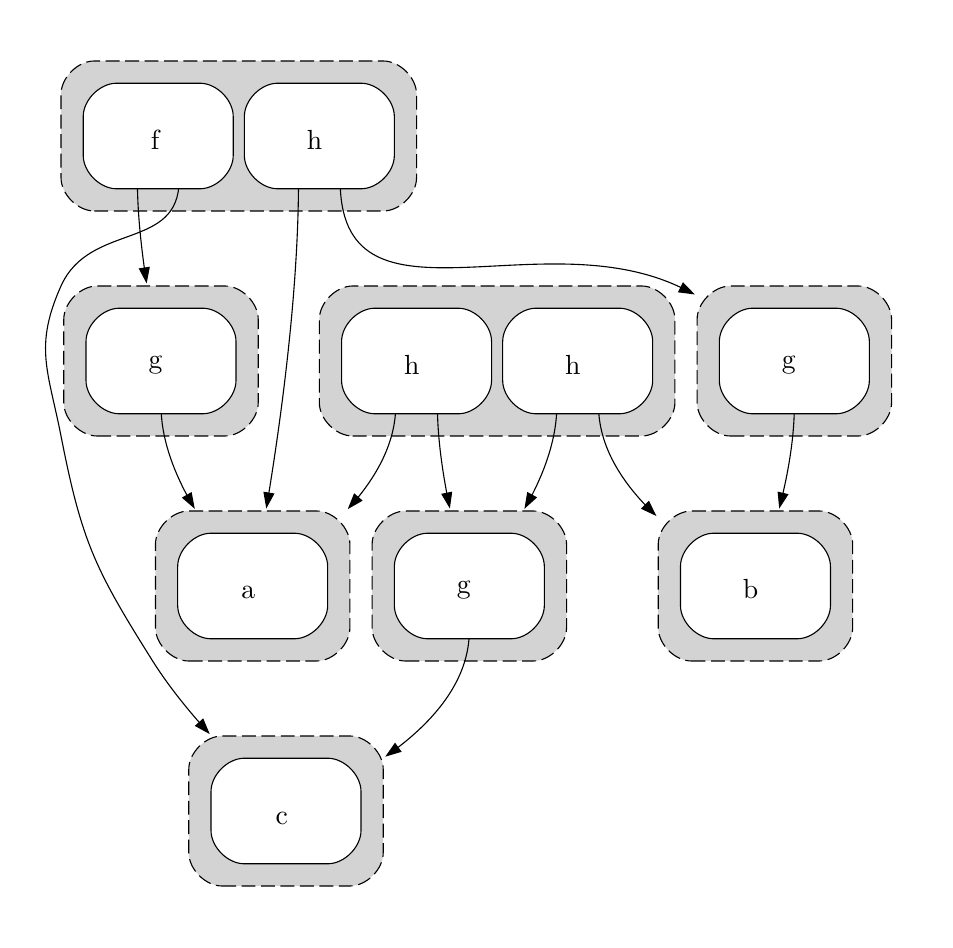
\begin{tikzpicture}[y=1cm, x=1cm, yscale=\globalscale,xscale=\globalscale, every node/.append style={scale=\globalscale}, inner sep=0pt, outer sep=0pt]
  \begin{scope}[shift={(0.1411, -11.1831)}]
    \path[fill=white] (-0.1411, 11.1831) -- (-0.1411, 22.5072) -- (11.2536, 22.5072) -- (11.2536, 11.1831) -- (-0.1411, 11.1831) -- (-0.1411, 11.1831)-- cycle;;



    \path[draw=black,fill=lightgrey,dash pattern=on 0.1764cm off 0.0706cm] (1.905, 14.4639).. controls (1.905, 14.4639) and (3.5278, 14.4639) .. (3.5278, 14.4639).. controls (3.7394, 14.4639) and (3.9511, 14.6756) .. (3.9511, 14.8872).. controls (3.9511, 14.8872) and (3.9511, 15.9456) .. (3.9511, 15.9456).. controls (3.9511, 16.1572) and (3.7394, 16.3689) .. (3.5278, 16.3689).. controls (3.5278, 16.3689) and (1.905, 16.3689) .. (1.905, 16.3689).. controls (1.6933, 16.3689) and (1.4817, 16.1572) .. (1.4817, 15.9456).. controls (1.4817, 15.9456) and (1.4817, 14.8872) .. (1.4817, 14.8872).. controls (1.4817, 14.6756) and (1.6933, 14.4639) .. (1.905, 14.4639);



    \path[draw=black,fill=lightgrey,dash pattern=on 0.1764cm off 0.0706cm] (0.7408, 17.3214).. controls (0.7408, 17.3214) and (2.3636, 17.3214) .. (2.3636, 17.3214).. controls (2.5753, 17.3214) and (2.7869, 17.5331) .. (2.7869, 17.7447).. controls (2.7869, 17.7447) and (2.7869, 18.8031) .. (2.7869, 18.8031).. controls (2.7869, 19.0147) and (2.5753, 19.2264) .. (2.3636, 19.2264).. controls (2.3636, 19.2264) and (0.7408, 19.2264) .. (0.7408, 19.2264).. controls (0.5292, 19.2264) and (0.3175, 19.0147) .. (0.3175, 18.8031).. controls (0.3175, 18.8031) and (0.3175, 17.7447) .. (0.3175, 17.7447).. controls (0.3175, 17.5331) and (0.5292, 17.3214) .. (0.7408, 17.3214);



    \path[draw=black,fill=lightgrey,dash pattern=on 0.1764cm off 0.0706cm] (2.3283, 11.6064).. controls (2.3283, 11.6064) and (3.9511, 11.6064) .. (3.9511, 11.6064).. controls (4.1628, 11.6064) and (4.3744, 11.8181) .. (4.3744, 12.0297).. controls (4.3744, 12.0297) and (4.3744, 13.0881) .. (4.3744, 13.0881).. controls (4.3744, 13.2997) and (4.1628, 13.5114) .. (3.9511, 13.5114).. controls (3.9511, 13.5114) and (2.3283, 13.5114) .. (2.3283, 13.5114).. controls (2.1167, 13.5114) and (1.905, 13.2997) .. (1.905, 13.0881).. controls (1.905, 13.0881) and (1.905, 12.0297) .. (1.905, 12.0297).. controls (1.905, 11.8181) and (2.1167, 11.6064) .. (2.3283, 11.6064);



    \path[draw=black,fill=lightgrey,dash pattern=on 0.1764cm off 0.0706cm] (0.7056, 20.1789).. controls (0.7056, 20.1789) and (4.3744, 20.1789) .. (4.3744, 20.1789).. controls (4.5861, 20.1789) and (4.7978, 20.3906) .. (4.7978, 20.6022).. controls (4.7978, 20.6022) and (4.7978, 21.6606) .. (4.7978, 21.6606).. controls (4.7978, 21.8722) and (4.5861, 22.0839) .. (4.3744, 22.0839).. controls (4.3744, 22.0839) and (0.7056, 22.0839) .. (0.7056, 22.0839).. controls (0.4939, 22.0839) and (0.2822, 21.8722) .. (0.2822, 21.6606).. controls (0.2822, 21.6606) and (0.2822, 20.6022) .. (0.2822, 20.6022).. controls (0.2822, 20.3906) and (0.4939, 20.1789) .. (0.7056, 20.1789);



    \path[draw=black,fill=lightgrey,dash pattern=on 0.1764cm off 0.0706cm] (8.2903, 14.4639).. controls (8.2903, 14.4639) and (9.9131, 14.4639) .. (9.9131, 14.4639).. controls (10.1247, 14.4639) and (10.3364, 14.6756) .. (10.3364, 14.8872).. controls (10.3364, 14.8872) and (10.3364, 15.9456) .. (10.3364, 15.9456).. controls (10.3364, 16.1572) and (10.1247, 16.3689) .. (9.9131, 16.3689).. controls (9.9131, 16.3689) and (8.2903, 16.3689) .. (8.2903, 16.3689).. controls (8.0786, 16.3689) and (7.8669, 16.1572) .. (7.8669, 15.9456).. controls (7.8669, 15.9456) and (7.8669, 14.8872) .. (7.8669, 14.8872).. controls (7.8669, 14.6756) and (8.0786, 14.4639) .. (8.2903, 14.4639);



    \path[draw=black,fill=lightgrey,dash pattern=on 0.1764cm off 0.0706cm] (8.7842, 17.3214).. controls (8.7842, 17.3214) and (10.4069, 17.3214) .. (10.4069, 17.3214).. controls (10.6186, 17.3214) and (10.8303, 17.5331) .. (10.8303, 17.7447).. controls (10.8303, 17.7447) and (10.8303, 18.8031) .. (10.8303, 18.8031).. controls (10.8303, 19.0147) and (10.6186, 19.2264) .. (10.4069, 19.2264).. controls (10.4069, 19.2264) and (8.7842, 19.2264) .. (8.7842, 19.2264).. controls (8.5725, 19.2264) and (8.3608, 19.0147) .. (8.3608, 18.8031).. controls (8.3608, 18.8031) and (8.3608, 17.7447) .. (8.3608, 17.7447).. controls (8.3608, 17.5331) and (8.5725, 17.3214) .. (8.7842, 17.3214);



    \path[draw=black,fill=lightgrey,dash pattern=on 0.1764cm off 0.0706cm] (4.6567, 14.4639).. controls (4.6567, 14.4639) and (6.2794, 14.4639) .. (6.2794, 14.4639).. controls (6.4911, 14.4639) and (6.7028, 14.6756) .. (6.7028, 14.8872).. controls (6.7028, 14.8872) and (6.7028, 15.9456) .. (6.7028, 15.9456).. controls (6.7028, 16.1572) and (6.4911, 16.3689) .. (6.2794, 16.3689).. controls (6.2794, 16.3689) and (4.6567, 16.3689) .. (4.6567, 16.3689).. controls (4.445, 16.3689) and (4.2333, 16.1572) .. (4.2333, 15.9456).. controls (4.2333, 15.9456) and (4.2333, 14.8872) .. (4.2333, 14.8872).. controls (4.2333, 14.6756) and (4.445, 14.4639) .. (4.6567, 14.4639);



    \path[draw=black,fill=lightgrey,dash pattern=on 0.1764cm off 0.0706cm] (3.9864, 17.3214).. controls (3.9864, 17.3214) and (7.6553, 17.3214) .. (7.6553, 17.3214).. controls (7.8669, 17.3214) and (8.0786, 17.5331) .. (8.0786, 17.7447).. controls (8.0786, 17.7447) and (8.0786, 18.8031) .. (8.0786, 18.8031).. controls (8.0786, 19.0147) and (7.8669, 19.2264) .. (7.6553, 19.2264).. controls (7.6553, 19.2264) and (3.9864, 19.2264) .. (3.9864, 19.2264).. controls (3.7747, 19.2264) and (3.5631, 19.0147) .. (3.5631, 18.8031).. controls (3.5631, 18.8031) and (3.5631, 17.7447) .. (3.5631, 17.7447).. controls (3.5631, 17.5331) and (3.7747, 17.3214) .. (3.9864, 17.3214);



    \path[draw=black] (1.5522, 17.7094).. controls (1.5522, 17.3126) and (1.6962, 16.9153) .. (1.8828, 16.5675);



    \path[draw=black,fill=black] (1.936, 16.5989) -- (1.9703, 16.4151) -- (1.8292, 16.5372) -- (1.936, 16.5989) -- (1.936, 16.5989)-- cycle;;



    \path[draw=black] (1.2524, 20.5669).. controls (1.2524, 20.1997) and (1.2919, 19.8018) .. (1.3423, 19.4433);



    \path[draw=black,fill=black] (1.4016, 19.4627) -- (1.3667, 19.2793) -- (1.2795, 19.4444) -- (1.4016, 19.4627) -- (1.4016, 19.4627)-- cycle;;



    \path[draw=black] (1.7815, 20.5669).. controls (1.7815, 19.673) and (0.6473, 20.0424) .. (0.2822, 19.2264).. controls (-0.0635, 18.4535) and (0.1196, 18.1522) .. (0.2822, 17.3214).. controls (0.5457, 15.9755) and (0.7161, 15.6249) .. (1.4464, 14.4639).. controls (1.6171, 14.1926) and (1.8284, 13.9234) .. (2.0436, 13.6775);



    \path[draw=black,fill=black] (2.0853, 13.7238) -- (2.1569, 13.5513) -- (1.9932, 13.6412) -- (2.0853, 13.7238) -- (2.0853, 13.7238)-- cycle;;



    \path[draw=black] (3.2985, 20.5669).. controls (3.2985, 19.1943) and (3.0889, 17.628) .. (2.9214, 16.594);



    \path[draw=black,fill=black] (2.9827, 16.5855) -- (2.8928, 16.4215) -- (2.8607, 16.6056) -- (2.9827, 16.5855) -- (2.9827, 16.5855)-- cycle;;



    \path[draw=black] (3.8276, 20.5669).. controls (3.8276, 18.5709) and (6.2985, 20.0561) .. (8.1139, 19.2264).. controls (8.1291, 19.2193) and (8.1446, 19.2123) .. (8.1601, 19.2049);



    \path[draw=black,fill=black] (8.183, 19.2624) -- (8.3132, 19.1283) -- (8.1276, 19.152) -- (8.183, 19.2624) -- (8.183, 19.2624)-- cycle;;



    \path[draw=black] (9.5956, 17.7094).. controls (9.5956, 17.3387) and (9.5314, 16.9411) .. (9.4488, 16.5848);



    \path[draw=black,fill=black] (9.5105, 16.5774) -- (9.4086, 16.4207) -- (9.3906, 16.6067) -- (9.5105, 16.5774) -- (9.5105, 16.5774)-- cycle;;



    \path[draw=black] (5.4681, 14.8519).. controls (5.4681, 14.236) and (5.043, 13.734) .. (4.5558, 13.3615);



    \path[draw=black,fill=black] (4.5967, 13.3149) -- (4.4175, 13.2613) -- (4.5244, 13.4147) -- (4.5967, 13.3149) -- (4.5967, 13.3149)-- cycle;;



    \path[draw=black] (4.5332, 17.7094).. controls (4.5332, 17.2748) and (4.3265, 16.8765) .. (4.0524, 16.5393);



    \path[draw=black,fill=black] (4.101, 16.5015) -- (3.9384, 16.4091) -- (4.0079, 16.5827) -- (4.101, 16.5015) -- (4.101, 16.5015)-- cycle;;



    \path[draw=black] (5.0624, 17.7094).. controls (5.0624, 17.3404) and (5.1156, 16.9425) .. (5.1834, 16.5855);



    \path[draw=black,fill=black] (5.2423, 16.6063) -- (5.2165, 16.4211) -- (5.1213, 16.5816) -- (5.2423, 16.6063) -- (5.2423, 16.6063)-- cycle;;



    \path[draw=black] (7.1085, 17.7094).. controls (7.1085, 17.2223) and (7.3723, 16.7908) .. (7.7082, 16.4387);



    \path[draw=black,fill=black] (7.7466, 16.4878) -- (7.8288, 16.3202) -- (7.6599, 16.3996) -- (7.7466, 16.4878) -- (7.7466, 16.4878)-- cycle;;



    \path[draw=black] (6.5793, 17.7094).. controls (6.5793, 17.3147) and (6.441, 16.9171) .. (6.2618, 16.5682);



    \path[draw=black,fill=black] (6.3168, 16.5407) -- (6.1778, 16.4155) -- (6.2085, 16.6) -- (6.3168, 16.5407) -- (6.3168, 16.5407)-- cycle;;



    \path[draw=black,fill=white] (3.2456, 16.0867).. controls (3.2456, 16.0867) and (2.1872, 16.0867) .. (2.1872, 16.0867).. controls (1.9756, 16.0867) and (1.7639, 15.875) .. (1.7639, 15.6633).. controls (1.7639, 15.6633) and (1.7639, 15.1694) .. (1.7639, 15.1694).. controls (1.7639, 14.9578) and (1.9756, 14.7461) .. (2.1872, 14.7461).. controls (2.1872, 14.7461) and (3.2456, 14.7461) .. (3.2456, 14.7461).. controls (3.4572, 14.7461) and (3.6689, 14.9578) .. (3.6689, 15.1694).. controls (3.6689, 15.1694) and (3.6689, 15.6633) .. (3.6689, 15.6633).. controls (3.6689, 15.875) and (3.4572, 16.0867) .. (3.2456, 16.0867);



    \node[anchor=south west] (text8469) at (2.571, 15.2516){a};



    \path[draw=black,fill=white] (2.0814, 18.9442).. controls (2.0814, 18.9442) and (1.0231, 18.9442) .. (1.0231, 18.9442).. controls (0.8114, 18.9442) and (0.5997, 18.7325) .. (0.5997, 18.5208).. controls (0.5997, 18.5208) and (0.5997, 18.0269) .. (0.5997, 18.0269).. controls (0.5997, 17.8153) and (0.8114, 17.6036) .. (1.0231, 17.6036).. controls (1.0231, 17.6036) and (2.0814, 17.6036) .. (2.0814, 17.6036).. controls (2.2931, 17.6036) and (2.5047, 17.8153) .. (2.5047, 18.0269).. controls (2.5047, 18.0269) and (2.5047, 18.5208) .. (2.5047, 18.5208).. controls (2.5047, 18.7325) and (2.2931, 18.9442) .. (2.0814, 18.9442);



    \node[anchor=south west] (text2456) at (1.3935, 18.1088){g};



    \path[draw=black,fill=white] (3.6689, 13.2292).. controls (3.6689, 13.2292) and (2.6106, 13.2292) .. (2.6106, 13.2292).. controls (2.3989, 13.2292) and (2.1872, 13.0175) .. (2.1872, 12.8058).. controls (2.1872, 12.8058) and (2.1872, 12.3119) .. (2.1872, 12.3119).. controls (2.1872, 12.1003) and (2.3989, 11.8886) .. (2.6106, 11.8886).. controls (2.6106, 11.8886) and (3.6689, 11.8886) .. (3.6689, 11.8886).. controls (3.8806, 11.8886) and (4.0922, 12.1003) .. (4.0922, 12.3119).. controls (4.0922, 12.3119) and (4.0922, 12.8058) .. (4.0922, 12.8058).. controls (4.0922, 13.0175) and (3.8806, 13.2292) .. (3.6689, 13.2292);



    \node[anchor=south west] (text463) at (3.0074, 12.3938){c};



    \path[draw=black,fill=white] (2.0461, 21.8017).. controls (2.0461, 21.8017) and (0.9878, 21.8017) .. (0.9878, 21.8017).. controls (0.7761, 21.8017) and (0.5644, 21.59) .. (0.5644, 21.3783).. controls (0.5644, 21.3783) and (0.5644, 20.8844) .. (0.5644, 20.8844).. controls (0.5644, 20.6728) and (0.7761, 20.4611) .. (0.9878, 20.4611).. controls (0.9878, 20.4611) and (2.0461, 20.4611) .. (2.0461, 20.4611).. controls (2.2578, 20.4611) and (2.4694, 20.6728) .. (2.4694, 20.8844).. controls (2.4694, 20.8844) and (2.4694, 21.3783) .. (2.4694, 21.3783).. controls (2.4694, 21.59) and (2.2578, 21.8017) .. (2.0461, 21.8017);



    \node[anchor=south west] (text7246) at (1.4245, 20.9663){f};



    \path[draw=black,fill=white] (4.0922, 21.8017).. controls (4.0922, 21.8017) and (3.0339, 21.8017) .. (3.0339, 21.8017).. controls (2.8222, 21.8017) and (2.6106, 21.59) .. (2.6106, 21.3783).. controls (2.6106, 21.3783) and (2.6106, 20.8844) .. (2.6106, 20.8844).. controls (2.6106, 20.6728) and (2.8222, 20.4611) .. (3.0339, 20.4611).. controls (3.0339, 20.4611) and (4.0922, 20.4611) .. (4.0922, 20.4611).. controls (4.3039, 20.4611) and (4.5156, 20.6728) .. (4.5156, 20.8844).. controls (4.5156, 20.8844) and (4.5156, 21.3783) .. (4.5156, 21.3783).. controls (4.5156, 21.59) and (4.3039, 21.8017) .. (4.0922, 21.8017);



    \node[anchor=south west] (text7118) at (3.4043, 20.9663){h};



    \path[draw=black,fill=white] (10.1247, 18.9442).. controls (10.1247, 18.9442) and (9.0664, 18.9442) .. (9.0664, 18.9442).. controls (8.8547, 18.9442) and (8.6431, 18.7325) .. (8.6431, 18.5208).. controls (8.6431, 18.5208) and (8.6431, 18.0269) .. (8.6431, 18.0269).. controls (8.6431, 17.8153) and (8.8547, 17.6036) .. (9.0664, 17.6036).. controls (9.0664, 17.6036) and (10.1247, 17.6036) .. (10.1247, 17.6036).. controls (10.3364, 17.6036) and (10.5481, 17.8153) .. (10.5481, 18.0269).. controls (10.5481, 18.0269) and (10.5481, 18.5208) .. (10.5481, 18.5208).. controls (10.5481, 18.7325) and (10.3364, 18.9442) .. (10.1247, 18.9442);



    \node[anchor=south west] (text3420) at (9.4368, 18.1088){g};



    \path[draw=black,fill=white] (9.6308, 16.0867).. controls (9.6308, 16.0867) and (8.5725, 16.0867) .. (8.5725, 16.0867).. controls (8.3608, 16.0867) and (8.1492, 15.875) .. (8.1492, 15.6633).. controls (8.1492, 15.6633) and (8.1492, 15.1694) .. (8.1492, 15.1694).. controls (8.1492, 14.9578) and (8.3608, 14.7461) .. (8.5725, 14.7461).. controls (8.5725, 14.7461) and (9.6308, 14.7461) .. (9.6308, 14.7461).. controls (9.8425, 14.7461) and (10.0542, 14.9578) .. (10.0542, 15.1694).. controls (10.0542, 15.1694) and (10.0542, 15.6633) .. (10.0542, 15.6633).. controls (10.0542, 15.875) and (9.8425, 16.0867) .. (9.6308, 16.0867);



    \node[anchor=south west] (text6905) at (8.9429, 15.2516){b};



    \path[draw=black,fill=white] (5.9972, 16.0867).. controls (5.9972, 16.0867) and (4.9389, 16.0867) .. (4.9389, 16.0867).. controls (4.7272, 16.0867) and (4.5156, 15.875) .. (4.5156, 15.6633).. controls (4.5156, 15.6633) and (4.5156, 15.1694) .. (4.5156, 15.1694).. controls (4.5156, 14.9578) and (4.7272, 14.7461) .. (4.9389, 14.7461).. controls (4.9389, 14.7461) and (5.9972, 14.7461) .. (5.9972, 14.7461).. controls (6.2089, 14.7461) and (6.4206, 14.9578) .. (6.4206, 15.1694).. controls (6.4206, 15.1694) and (6.4206, 15.6633) .. (6.4206, 15.6633).. controls (6.4206, 15.875) and (6.2089, 16.0867) .. (5.9972, 16.0867);



    \node[anchor=south west] (text4845) at (5.3093, 15.2516){g};



    \path[draw=black,fill=white] (5.3269, 18.9442).. controls (5.3269, 18.9442) and (4.2686, 18.9442) .. (4.2686, 18.9442).. controls (4.0569, 18.9442) and (3.8453, 18.7325) .. (3.8453, 18.5208).. controls (3.8453, 18.5208) and (3.8453, 18.0269) .. (3.8453, 18.0269).. controls (3.8453, 17.8153) and (4.0569, 17.6036) .. (4.2686, 17.6036).. controls (4.2686, 17.6036) and (5.3269, 17.6036) .. (5.3269, 17.6036).. controls (5.5386, 17.6036) and (5.7503, 17.8153) .. (5.7503, 18.0269).. controls (5.7503, 18.0269) and (5.7503, 18.5208) .. (5.7503, 18.5208).. controls (5.7503, 18.7325) and (5.5386, 18.9442) .. (5.3269, 18.9442);



    \node[anchor=south west] (text8176) at (4.639, 18.1088){h};



    \path[draw=black,fill=white] (7.3731, 18.9442).. controls (7.3731, 18.9442) and (6.3147, 18.9442) .. (6.3147, 18.9442).. controls (6.1031, 18.9442) and (5.8914, 18.7325) .. (5.8914, 18.5208).. controls (5.8914, 18.5208) and (5.8914, 18.0269) .. (5.8914, 18.0269).. controls (5.8914, 17.8153) and (6.1031, 17.6036) .. (6.3147, 17.6036).. controls (6.3147, 17.6036) and (7.3731, 17.6036) .. (7.3731, 17.6036).. controls (7.5847, 17.6036) and (7.7964, 17.8153) .. (7.7964, 18.0269).. controls (7.7964, 18.0269) and (7.7964, 18.5208) .. (7.7964, 18.5208).. controls (7.7964, 18.7325) and (7.5847, 18.9442) .. (7.3731, 18.9442);



    \node[anchor=south west] (text4894) at (6.6851, 18.1088){h};



  \end{scope}

\end{tikzpicture}
\label{exampleBasic4}
\end{center}

Now we handle \ref{examplecc3}, which doesn't add any new E-nodes in the graph. Instead, it merges the separate E-classes representing $g(b)$ and $g(c)$ into a single E-node.

\begin{center}
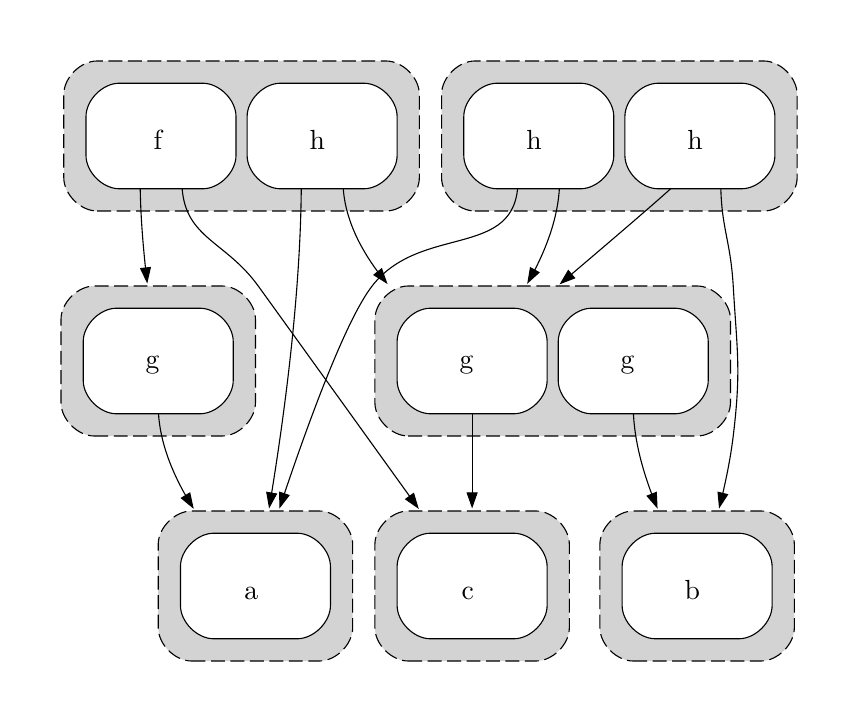
\begin{tikzpicture}[y=1cm, x=1cm, yscale=\globalscale,xscale=\globalscale, every node/.append style={scale=\globalscale}, inner sep=0pt, outer sep=0pt]
  \begin{scope}[shift={(0.1411, -8.3256)}]
    \path[fill=white] (-0.1411, 8.3256) -- (-0.1411, 16.7922) -- (10.0542, 16.7922) -- (10.0542, 8.3256) -- (-0.1411, 8.3256) -- (-0.1411, 8.3256)-- cycle;;



    \path[draw=black,fill=lightgrey,dash pattern=on 0.1764cm off 0.0706cm] (1.9403, 8.7489).. controls (1.9403, 8.7489) and (3.5631, 8.7489) .. (3.5631, 8.7489).. controls (3.7747, 8.7489) and (3.9864, 8.9606) .. (3.9864, 9.1722).. controls (3.9864, 9.1722) and (3.9864, 10.2306) .. (3.9864, 10.2306).. controls (3.9864, 10.4422) and (3.7747, 10.6539) .. (3.5631, 10.6539).. controls (3.5631, 10.6539) and (1.9403, 10.6539) .. (1.9403, 10.6539).. controls (1.7286, 10.6539) and (1.5169, 10.4422) .. (1.5169, 10.2306).. controls (1.5169, 10.2306) and (1.5169, 9.1722) .. (1.5169, 9.1722).. controls (1.5169, 8.9606) and (1.7286, 8.7489) .. (1.9403, 8.7489);



    \path[draw=black,fill=lightgrey,dash pattern=on 0.1764cm off 0.0706cm] (0.7056, 11.6064).. controls (0.7056, 11.6064) and (2.3283, 11.6064) .. (2.3283, 11.6064).. controls (2.54, 11.6064) and (2.7517, 11.8181) .. (2.7517, 12.0297).. controls (2.7517, 12.0297) and (2.7517, 13.0881) .. (2.7517, 13.0881).. controls (2.7517, 13.2997) and (2.54, 13.5114) .. (2.3283, 13.5114).. controls (2.3283, 13.5114) and (0.7056, 13.5114) .. (0.7056, 13.5114).. controls (0.4939, 13.5114) and (0.2822, 13.2997) .. (0.2822, 13.0881).. controls (0.2822, 13.0881) and (0.2822, 12.0297) .. (0.2822, 12.0297).. controls (0.2822, 11.8181) and (0.4939, 11.6064) .. (0.7056, 11.6064);



    \path[draw=black,fill=lightgrey,dash pattern=on 0.1764cm off 0.0706cm] (4.6919, 8.7489).. controls (4.6919, 8.7489) and (6.3147, 8.7489) .. (6.3147, 8.7489).. controls (6.5264, 8.7489) and (6.7381, 8.9606) .. (6.7381, 9.1722).. controls (6.7381, 9.1722) and (6.7381, 10.2306) .. (6.7381, 10.2306).. controls (6.7381, 10.4422) and (6.5264, 10.6539) .. (6.3147, 10.6539).. controls (6.3147, 10.6539) and (4.6919, 10.6539) .. (4.6919, 10.6539).. controls (4.4803, 10.6539) and (4.2686, 10.4422) .. (4.2686, 10.2306).. controls (4.2686, 10.2306) and (4.2686, 9.1722) .. (4.2686, 9.1722).. controls (4.2686, 8.9606) and (4.4803, 8.7489) .. (4.6919, 8.7489);



    \path[draw=black,fill=lightgrey,dash pattern=on 0.1764cm off 0.0706cm] (0.7408, 14.4639).. controls (0.7408, 14.4639) and (4.4097, 14.4639) .. (4.4097, 14.4639).. controls (4.6214, 14.4639) and (4.8331, 14.6756) .. (4.8331, 14.8872).. controls (4.8331, 14.8872) and (4.8331, 15.9456) .. (4.8331, 15.9456).. controls (4.8331, 16.1572) and (4.6214, 16.3689) .. (4.4097, 16.3689).. controls (4.4097, 16.3689) and (0.7408, 16.3689) .. (0.7408, 16.3689).. controls (0.5292, 16.3689) and (0.3175, 16.1572) .. (0.3175, 15.9456).. controls (0.3175, 15.9456) and (0.3175, 14.8872) .. (0.3175, 14.8872).. controls (0.3175, 14.6756) and (0.5292, 14.4639) .. (0.7408, 14.4639);



    \path[draw=black,fill=lightgrey,dash pattern=on 0.1764cm off 0.0706cm] (7.5494, 8.7489).. controls (7.5494, 8.7489) and (9.1722, 8.7489) .. (9.1722, 8.7489).. controls (9.3839, 8.7489) and (9.5956, 8.9606) .. (9.5956, 9.1722).. controls (9.5956, 9.1722) and (9.5956, 10.2306) .. (9.5956, 10.2306).. controls (9.5956, 10.4422) and (9.3839, 10.6539) .. (9.1722, 10.6539).. controls (9.1722, 10.6539) and (7.5494, 10.6539) .. (7.5494, 10.6539).. controls (7.3378, 10.6539) and (7.1261, 10.4422) .. (7.1261, 10.2306).. controls (7.1261, 10.2306) and (7.1261, 9.1722) .. (7.1261, 9.1722).. controls (7.1261, 8.9606) and (7.3378, 8.7489) .. (7.5494, 8.7489);



    \path[draw=black,fill=lightgrey,dash pattern=on 0.1764cm off 0.0706cm] (4.6919, 11.6064).. controls (4.6919, 11.6064) and (8.3608, 11.6064) .. (8.3608, 11.6064).. controls (8.5725, 11.6064) and (8.7842, 11.8181) .. (8.7842, 12.0297).. controls (8.7842, 12.0297) and (8.7842, 13.0881) .. (8.7842, 13.0881).. controls (8.7842, 13.2997) and (8.5725, 13.5114) .. (8.3608, 13.5114).. controls (8.3608, 13.5114) and (4.6919, 13.5114) .. (4.6919, 13.5114).. controls (4.4803, 13.5114) and (4.2686, 13.2997) .. (4.2686, 13.0881).. controls (4.2686, 13.0881) and (4.2686, 12.0297) .. (4.2686, 12.0297).. controls (4.2686, 11.8181) and (4.4803, 11.6064) .. (4.6919, 11.6064);



    \path[draw=black,fill=lightgrey,dash pattern=on 0.1764cm off 0.0706cm] (5.5386, 14.4639).. controls (5.5386, 14.4639) and (9.2075, 14.4639) .. (9.2075, 14.4639).. controls (9.4192, 14.4639) and (9.6308, 14.6756) .. (9.6308, 14.8872).. controls (9.6308, 14.8872) and (9.6308, 15.9456) .. (9.6308, 15.9456).. controls (9.6308, 16.1572) and (9.4192, 16.3689) .. (9.2075, 16.3689).. controls (9.2075, 16.3689) and (5.5386, 16.3689) .. (5.5386, 16.3689).. controls (5.3269, 16.3689) and (5.1153, 16.1572) .. (5.1153, 15.9456).. controls (5.1153, 15.9456) and (5.1153, 14.8872) .. (5.1153, 14.8872).. controls (5.1153, 14.6756) and (5.3269, 14.4639) .. (5.5386, 14.4639);



    \path[draw=black] (1.5169, 11.9944).. controls (1.5169, 11.5905) and (1.6708, 11.1905) .. (1.8701, 10.8419);



    \path[draw=black,fill=black] (1.9177, 10.8821) -- (1.9569, 10.6994) -- (1.8122, 10.8179) -- (1.9177, 10.8821) -- (1.9177, 10.8821)-- cycle;;



    \path[draw=black] (1.2876, 14.8519).. controls (1.2876, 14.4889) and (1.3173, 14.0949) .. (1.3554, 13.7389);



    \path[draw=black,fill=black] (1.4168, 13.7467) -- (1.3751, 13.5643) -- (1.294, 13.7326) -- (1.4168, 13.7467) -- (1.4168, 13.7467)-- cycle;;



    \path[draw=black] (1.8168, 14.8519).. controls (1.8168, 14.1164) and (2.3566, 14.1079) .. (2.7869, 13.5114).. controls (3.4357, 12.6125) and (4.1695, 11.5923) .. (4.711, 10.8395);



    \path[draw=black,fill=black] (4.7604, 10.8765) -- (4.8133, 10.6973) -- (4.6602, 10.8045) -- (4.7604, 10.8765) -- (4.7604, 10.8765)-- cycle;;



    \path[draw=black] (3.3338, 14.8519).. controls (3.3338, 13.4793) and (3.1242, 11.913) .. (2.9566, 10.879);



    \path[draw=black,fill=black] (3.018, 10.8705) -- (2.9281, 10.7065) -- (2.896, 10.8906) -- (3.018, 10.8705) -- (3.018, 10.8705)-- cycle;;



    \path[draw=black] (3.8629, 14.8519).. controls (3.8629, 14.4258) and (4.0566, 14.0257) .. (4.3109, 13.6843);



    \path[draw=black,fill=black] (4.354, 13.7294) -- (4.4157, 13.553) -- (4.2573, 13.6525) -- (4.354, 13.7294) -- (4.354, 13.7294)-- cycle;;



    \path[draw=black] (5.5033, 11.9944).. controls (5.5033, 11.6325) and (5.5033, 11.2384) .. (5.5033, 10.8818);



    \path[draw=black,fill=black] (5.5651, 10.8835) -- (5.5033, 10.7072) -- (5.4416, 10.8835) -- (5.5651, 10.8835) -- (5.5651, 10.8835)-- cycle;;



    \path[draw=black] (7.5494, 11.9944).. controls (7.5494, 11.6145) and (7.6525, 11.219) .. (7.7851, 10.867);



    \path[draw=black,fill=black] (7.8422, 10.8899) -- (7.8507, 10.7033) -- (7.7276, 10.844) -- (7.8422, 10.8899) -- (7.8422, 10.8899)-- cycle;;



    \path[draw=black] (6.0854, 14.8519).. controls (6.0854, 13.8359) and (4.8556, 14.3147) .. (4.2333, 13.5114).. controls (3.9024, 13.0845) and (3.4361, 11.8135) .. (3.1154, 10.8634);



    \path[draw=black,fill=black] (3.1768, 10.8521) -- (3.0621, 10.7043) -- (3.0596, 10.8913) -- (3.1768, 10.8521) -- (3.1768, 10.8521)-- cycle;;



    \path[draw=black] (6.6146, 14.8519).. controls (6.6146, 14.4572) and (6.4763, 14.0596) .. (6.2971, 13.7107);



    \path[draw=black,fill=black] (6.3521, 13.6832) -- (6.2131, 13.558) -- (6.2438, 13.7425) -- (6.3521, 13.6832) -- (6.3521, 13.6832)-- cycle;;



    \path[draw=black] (8.1315, 14.8519).. controls (8.1315, 14.8273) and (7.4358, 14.23) .. (6.7603, 13.6564);



    \path[draw=black,fill=black] (6.8044, 13.613) -- (6.6301, 13.546) -- (6.7247, 13.7072) -- (6.8044, 13.613) -- (6.8044, 13.613)-- cycle;;



    \path[draw=black] (8.6607, 14.8519).. controls (8.6607, 14.2519) and (8.7842, 14.1104) .. (8.8194, 13.5114).. controls (8.8692, 12.6661) and (8.921, 12.4471) .. (8.8194, 11.6064).. controls (8.7905, 11.3658) and (8.7411, 11.1114) .. (8.685, 10.8705);



    \path[draw=black,fill=black] (8.7468, 10.8624) -- (8.6448, 10.7057) -- (8.6268, 10.8917) -- (8.7468, 10.8624) -- (8.7468, 10.8624)-- cycle;;



    \path[draw=black,fill=white] (3.2808, 10.3717).. controls (3.2808, 10.3717) and (2.2225, 10.3717) .. (2.2225, 10.3717).. controls (2.0108, 10.3717) and (1.7992, 10.16) .. (1.7992, 9.9483).. controls (1.7992, 9.9483) and (1.7992, 9.4544) .. (1.7992, 9.4544).. controls (1.7992, 9.2428) and (2.0108, 9.0311) .. (2.2225, 9.0311).. controls (2.2225, 9.0311) and (3.2808, 9.0311) .. (3.2808, 9.0311).. controls (3.4925, 9.0311) and (3.7042, 9.2428) .. (3.7042, 9.4544).. controls (3.7042, 9.4544) and (3.7042, 9.9483) .. (3.7042, 9.9483).. controls (3.7042, 10.16) and (3.4925, 10.3717) .. (3.2808, 10.3717);



    \node[anchor=south west] (text6692) at (2.6063, 9.5363){a};



    \path[draw=black,fill=white] (2.0461, 13.2292).. controls (2.0461, 13.2292) and (0.9878, 13.2292) .. (0.9878, 13.2292).. controls (0.7761, 13.2292) and (0.5644, 13.0175) .. (0.5644, 12.8058).. controls (0.5644, 12.8058) and (0.5644, 12.3119) .. (0.5644, 12.3119).. controls (0.5644, 12.1003) and (0.7761, 11.8886) .. (0.9878, 11.8886).. controls (0.9878, 11.8886) and (2.0461, 11.8886) .. (2.0461, 11.8886).. controls (2.2578, 11.8886) and (2.4694, 12.1003) .. (2.4694, 12.3119).. controls (2.4694, 12.3119) and (2.4694, 12.8058) .. (2.4694, 12.8058).. controls (2.4694, 13.0175) and (2.2578, 13.2292) .. (2.0461, 13.2292);



    \node[anchor=south west] (text4814) at (1.3582, 12.3941){g};



    \path[draw=black,fill=white] (6.0325, 10.3717).. controls (6.0325, 10.3717) and (4.9742, 10.3717) .. (4.9742, 10.3717).. controls (4.7625, 10.3717) and (4.5508, 10.16) .. (4.5508, 9.9483).. controls (4.5508, 9.9483) and (4.5508, 9.4544) .. (4.5508, 9.4544).. controls (4.5508, 9.2428) and (4.7625, 9.0311) .. (4.9742, 9.0311).. controls (4.9742, 9.0311) and (6.0325, 9.0311) .. (6.0325, 9.0311).. controls (6.2442, 9.0311) and (6.4558, 9.2428) .. (6.4558, 9.4544).. controls (6.4558, 9.4544) and (6.4558, 9.9483) .. (6.4558, 9.9483).. controls (6.4558, 10.16) and (6.2442, 10.3717) .. (6.0325, 10.3717);



    \node[anchor=south west] (text4236) at (5.371, 9.5363){c};



    \path[draw=black,fill=white] (2.0814, 16.0867).. controls (2.0814, 16.0867) and (1.0231, 16.0867) .. (1.0231, 16.0867).. controls (0.8114, 16.0867) and (0.5997, 15.875) .. (0.5997, 15.6633).. controls (0.5997, 15.6633) and (0.5997, 15.1694) .. (0.5997, 15.1694).. controls (0.5997, 14.9578) and (0.8114, 14.7461) .. (1.0231, 14.7461).. controls (1.0231, 14.7461) and (2.0814, 14.7461) .. (2.0814, 14.7461).. controls (2.2931, 14.7461) and (2.5047, 14.9578) .. (2.5047, 15.1694).. controls (2.5047, 15.1694) and (2.5047, 15.6633) .. (2.5047, 15.6633).. controls (2.5047, 15.875) and (2.2931, 16.0867) .. (2.0814, 16.0867);



    \node[anchor=south west] (text3516) at (1.4598, 15.2513){f};



    \path[draw=black,fill=white] (4.1275, 16.0867).. controls (4.1275, 16.0867) and (3.0692, 16.0867) .. (3.0692, 16.0867).. controls (2.8575, 16.0867) and (2.6458, 15.875) .. (2.6458, 15.6633).. controls (2.6458, 15.6633) and (2.6458, 15.1694) .. (2.6458, 15.1694).. controls (2.6458, 14.9578) and (2.8575, 14.7461) .. (3.0692, 14.7461).. controls (3.0692, 14.7461) and (4.1275, 14.7461) .. (4.1275, 14.7461).. controls (4.3392, 14.7461) and (4.5508, 14.9578) .. (4.5508, 15.1694).. controls (4.5508, 15.1694) and (4.5508, 15.6633) .. (4.5508, 15.6633).. controls (4.5508, 15.875) and (4.3392, 16.0867) .. (4.1275, 16.0867);



    \node[anchor=south west] (text6697) at (3.4396, 15.2513){h};



    \path[draw=black,fill=white] (6.0325, 13.2292).. controls (6.0325, 13.2292) and (4.9742, 13.2292) .. (4.9742, 13.2292).. controls (4.7625, 13.2292) and (4.5508, 13.0175) .. (4.5508, 12.8058).. controls (4.5508, 12.8058) and (4.5508, 12.3119) .. (4.5508, 12.3119).. controls (4.5508, 12.1003) and (4.7625, 11.8886) .. (4.9742, 11.8886).. controls (4.9742, 11.8886) and (6.0325, 11.8886) .. (6.0325, 11.8886).. controls (6.2442, 11.8886) and (6.4558, 12.1003) .. (6.4558, 12.3119).. controls (6.4558, 12.3119) and (6.4558, 12.8058) .. (6.4558, 12.8058).. controls (6.4558, 13.0175) and (6.2442, 13.2292) .. (6.0325, 13.2292);



    \node[anchor=south west] (text264) at (5.3446, 12.3941){g};



    \path[draw=black,fill=white] (8.89, 10.3717).. controls (8.89, 10.3717) and (7.8317, 10.3717) .. (7.8317, 10.3717).. controls (7.62, 10.3717) and (7.4083, 10.16) .. (7.4083, 9.9483).. controls (7.4083, 9.9483) and (7.4083, 9.4544) .. (7.4083, 9.4544).. controls (7.4083, 9.2428) and (7.62, 9.0311) .. (7.8317, 9.0311).. controls (7.8317, 9.0311) and (8.89, 9.0311) .. (8.89, 9.0311).. controls (9.1017, 9.0311) and (9.3133, 9.2428) .. (9.3133, 9.4544).. controls (9.3133, 9.4544) and (9.3133, 9.9483) .. (9.3133, 9.9483).. controls (9.3133, 10.16) and (9.1017, 10.3717) .. (8.89, 10.3717);



    \node[anchor=south west] (text1129) at (8.2021, 9.5363){b};



    \path[draw=black,fill=white] (8.0786, 13.2292).. controls (8.0786, 13.2292) and (7.0203, 13.2292) .. (7.0203, 13.2292).. controls (6.8086, 13.2292) and (6.5969, 13.0175) .. (6.5969, 12.8058).. controls (6.5969, 12.8058) and (6.5969, 12.3119) .. (6.5969, 12.3119).. controls (6.5969, 12.1003) and (6.8086, 11.8886) .. (7.0203, 11.8886).. controls (7.0203, 11.8886) and (8.0786, 11.8886) .. (8.0786, 11.8886).. controls (8.2903, 11.8886) and (8.5019, 12.1003) .. (8.5019, 12.3119).. controls (8.5019, 12.3119) and (8.5019, 12.8058) .. (8.5019, 12.8058).. controls (8.5019, 13.0175) and (8.2903, 13.2292) .. (8.0786, 13.2292);



    \node[anchor=south west] (text318) at (7.3907, 12.3941){g};



    \path[draw=black,fill=white] (6.8792, 16.0867).. controls (6.8792, 16.0867) and (5.8208, 16.0867) .. (5.8208, 16.0867).. controls (5.6092, 16.0867) and (5.3975, 15.875) .. (5.3975, 15.6633).. controls (5.3975, 15.6633) and (5.3975, 15.1694) .. (5.3975, 15.1694).. controls (5.3975, 14.9578) and (5.6092, 14.7461) .. (5.8208, 14.7461).. controls (5.8208, 14.7461) and (6.8792, 14.7461) .. (6.8792, 14.7461).. controls (7.0908, 14.7461) and (7.3025, 14.9578) .. (7.3025, 15.1694).. controls (7.3025, 15.1694) and (7.3025, 15.6633) .. (7.3025, 15.6633).. controls (7.3025, 15.875) and (7.0908, 16.0867) .. (6.8792, 16.0867);



    \node[anchor=south west] (text5846) at (6.1913, 15.2513){h};



    \path[draw=black,fill=white] (8.9253, 16.0867).. controls (8.9253, 16.0867) and (7.8669, 16.0867) .. (7.8669, 16.0867).. controls (7.6553, 16.0867) and (7.4436, 15.875) .. (7.4436, 15.6633).. controls (7.4436, 15.6633) and (7.4436, 15.1694) .. (7.4436, 15.1694).. controls (7.4436, 14.9578) and (7.6553, 14.7461) .. (7.8669, 14.7461).. controls (7.8669, 14.7461) and (8.9253, 14.7461) .. (8.9253, 14.7461).. controls (9.1369, 14.7461) and (9.3486, 14.9578) .. (9.3486, 15.1694).. controls (9.3486, 15.1694) and (9.3486, 15.6633) .. (9.3486, 15.6633).. controls (9.3486, 15.875) and (9.1369, 16.0867) .. (8.9253, 16.0867);



    \node[anchor=south west] (text8361) at (8.2374, 15.2513){h};



  \end{scope}

\end{tikzpicture}
\label{exampleBasic5}
\end{center}

Now notice that we have two instances of an $h$ with the same arguments: $h(a, g(b)$ and $h(a, g(c)$ have become equal by congruence, but they are located in two different E-classes. So, after unioning, we need to \emph{propagate} by continuing to union things that have become equal. This gives us the simpler E-graph

\begin{center}
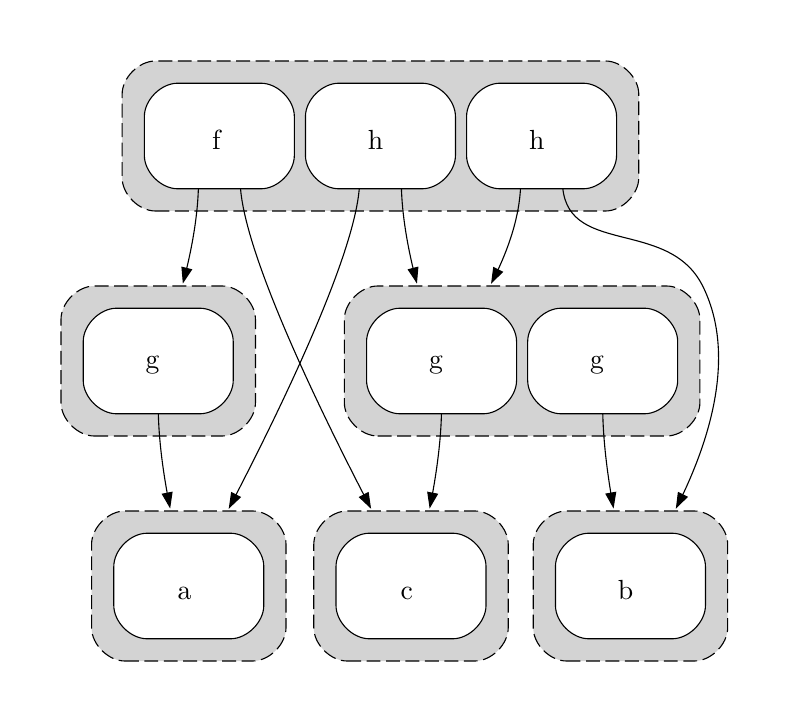
\begin{tikzpicture}[y=1cm, x=1cm, yscale=\globalscale,xscale=\globalscale, every node/.append style={scale=\globalscale}, inner sep=0pt, outer sep=0pt]
  \begin{scope}[shift={(0.1411, -8.3256)}]
    \path[fill=white] (-0.1411, 8.3256) -- (-0.1411, 16.7922) -- (9.1722, 16.7922) -- (9.1722, 8.3256) -- (-0.1411, 8.3256) -- (-0.1411, 8.3256)-- cycle;;



    \path[draw=black,fill=lightgrey,dash pattern=on 0.1764cm off 0.0706cm] (1.0936, 8.7489).. controls (1.0936, 8.7489) and (2.7164, 8.7489) .. (2.7164, 8.7489).. controls (2.9281, 8.7489) and (3.1397, 8.9606) .. (3.1397, 9.1722).. controls (3.1397, 9.1722) and (3.1397, 10.2306) .. (3.1397, 10.2306).. controls (3.1397, 10.4422) and (2.9281, 10.6539) .. (2.7164, 10.6539).. controls (2.7164, 10.6539) and (1.0936, 10.6539) .. (1.0936, 10.6539).. controls (0.8819, 10.6539) and (0.6703, 10.4422) .. (0.6703, 10.2306).. controls (0.6703, 10.2306) and (0.6703, 9.1722) .. (0.6703, 9.1722).. controls (0.6703, 8.9606) and (0.8819, 8.7489) .. (1.0936, 8.7489);



    \path[draw=black,fill=lightgrey,dash pattern=on 0.1764cm off 0.0706cm] (0.7056, 11.6064).. controls (0.7056, 11.6064) and (2.3283, 11.6064) .. (2.3283, 11.6064).. controls (2.54, 11.6064) and (2.7517, 11.8181) .. (2.7517, 12.0297).. controls (2.7517, 12.0297) and (2.7517, 13.0881) .. (2.7517, 13.0881).. controls (2.7517, 13.2997) and (2.54, 13.5114) .. (2.3283, 13.5114).. controls (2.3283, 13.5114) and (0.7056, 13.5114) .. (0.7056, 13.5114).. controls (0.4939, 13.5114) and (0.2822, 13.2997) .. (0.2822, 13.0881).. controls (0.2822, 13.0881) and (0.2822, 12.0297) .. (0.2822, 12.0297).. controls (0.2822, 11.8181) and (0.4939, 11.6064) .. (0.7056, 11.6064);



    \path[draw=black,fill=lightgrey,dash pattern=on 0.1764cm off 0.0706cm] (3.9158, 8.7489).. controls (3.9158, 8.7489) and (5.5386, 8.7489) .. (5.5386, 8.7489).. controls (5.7503, 8.7489) and (5.9619, 8.9606) .. (5.9619, 9.1722).. controls (5.9619, 9.1722) and (5.9619, 10.2306) .. (5.9619, 10.2306).. controls (5.9619, 10.4422) and (5.7503, 10.6539) .. (5.5386, 10.6539).. controls (5.5386, 10.6539) and (3.9158, 10.6539) .. (3.9158, 10.6539).. controls (3.7042, 10.6539) and (3.4925, 10.4422) .. (3.4925, 10.2306).. controls (3.4925, 10.2306) and (3.4925, 9.1722) .. (3.4925, 9.1722).. controls (3.4925, 8.9606) and (3.7042, 8.7489) .. (3.9158, 8.7489);



    \path[draw=black,fill=lightgrey,dash pattern=on 0.1764cm off 0.0706cm] (1.4817, 14.4639).. controls (1.4817, 14.4639) and (7.1967, 14.4639) .. (7.1967, 14.4639).. controls (7.4083, 14.4639) and (7.62, 14.6756) .. (7.62, 14.8872).. controls (7.62, 14.8872) and (7.62, 15.9456) .. (7.62, 15.9456).. controls (7.62, 16.1572) and (7.4083, 16.3689) .. (7.1967, 16.3689).. controls (7.1967, 16.3689) and (1.4817, 16.3689) .. (1.4817, 16.3689).. controls (1.27, 16.3689) and (1.0583, 16.1572) .. (1.0583, 15.9456).. controls (1.0583, 15.9456) and (1.0583, 14.8872) .. (1.0583, 14.8872).. controls (1.0583, 14.6756) and (1.27, 14.4639) .. (1.4817, 14.4639);



    \path[draw=black,fill=lightgrey,dash pattern=on 0.1764cm off 0.0706cm] (6.7028, 8.7489).. controls (6.7028, 8.7489) and (8.3256, 8.7489) .. (8.3256, 8.7489).. controls (8.5372, 8.7489) and (8.7489, 8.9606) .. (8.7489, 9.1722).. controls (8.7489, 9.1722) and (8.7489, 10.2306) .. (8.7489, 10.2306).. controls (8.7489, 10.4422) and (8.5372, 10.6539) .. (8.3256, 10.6539).. controls (8.3256, 10.6539) and (6.7028, 10.6539) .. (6.7028, 10.6539).. controls (6.4911, 10.6539) and (6.2794, 10.4422) .. (6.2794, 10.2306).. controls (6.2794, 10.2306) and (6.2794, 9.1722) .. (6.2794, 9.1722).. controls (6.2794, 8.9606) and (6.4911, 8.7489) .. (6.7028, 8.7489);



    \path[draw=black,fill=lightgrey,dash pattern=on 0.1764cm off 0.0706cm] (4.3039, 11.6064).. controls (4.3039, 11.6064) and (7.9728, 11.6064) .. (7.9728, 11.6064).. controls (8.1844, 11.6064) and (8.3961, 11.8181) .. (8.3961, 12.0297).. controls (8.3961, 12.0297) and (8.3961, 13.0881) .. (8.3961, 13.0881).. controls (8.3961, 13.2997) and (8.1844, 13.5114) .. (7.9728, 13.5114).. controls (7.9728, 13.5114) and (4.3039, 13.5114) .. (4.3039, 13.5114).. controls (4.0922, 13.5114) and (3.8806, 13.2997) .. (3.8806, 13.0881).. controls (3.8806, 13.0881) and (3.8806, 12.0297) .. (3.8806, 12.0297).. controls (3.8806, 11.8181) and (4.0922, 11.6064) .. (4.3039, 11.6064);



    \path[draw=black] (1.5169, 11.9944).. controls (1.5169, 11.6258) and (1.5677, 11.2279) .. (1.6327, 10.8705);



    \path[draw=black,fill=black] (1.6916, 10.8913) -- (1.6644, 10.7065) -- (1.5706, 10.8677) -- (1.6916, 10.8913) -- (1.6916, 10.8913)-- cycle;;



    \path[draw=black] (2.0285, 14.8519).. controls (2.0285, 14.4808) and (1.9618, 14.0832) .. (1.8768, 13.7273);



    \path[draw=black,fill=black] (1.9382, 13.7188) -- (1.8348, 13.5629) -- (1.8186, 13.7492) -- (1.9382, 13.7188) -- (1.9382, 13.7188)-- cycle;;



    \path[draw=black] (2.5576, 14.8519).. controls (2.5576, 14.0416) and (3.4918, 12.0918) .. (4.1342, 10.8472);



    \path[draw=black,fill=black] (4.1836, 10.8864) -- (4.2101, 10.7012) -- (4.0742, 10.8292) -- (4.1836, 10.8864) -- (4.1836, 10.8864)-- cycle;;



    \path[draw=black] (4.0746, 14.8519).. controls (4.0746, 14.0416) and (3.1404, 12.0918) .. (2.498, 10.8472);



    \path[draw=black,fill=black] (2.558, 10.8292) -- (2.4222, 10.7012) -- (2.4486, 10.8864) -- (2.558, 10.8292) -- (2.558, 10.8292)-- cycle;;



    \path[draw=black] (4.6038, 14.8519).. controls (4.6038, 14.4808) and (4.6704, 14.0832) .. (4.7554, 13.7273);



    \path[draw=black,fill=black] (4.8137, 13.7492) -- (4.7974, 13.5629) -- (4.6941, 13.7188) -- (4.8137, 13.7492) -- (4.8137, 13.7492)-- cycle;;



    \path[draw=black] (5.1153, 11.9944).. controls (5.1153, 11.6258) and (5.0645, 11.2279) .. (4.9996, 10.8705);



    \path[draw=black,fill=black] (5.0617, 10.8677) -- (4.9678, 10.7065) -- (4.9407, 10.8913) -- (5.0617, 10.8677) -- (5.0617, 10.8677)-- cycle;;



    \path[draw=black] (6.1207, 14.8519).. controls (6.1207, 14.4614) and (5.9937, 14.0631) .. (5.8297, 13.7121);



    \path[draw=black,fill=black] (5.8875, 13.6895) -- (5.7535, 13.559) -- (5.7771, 13.7446) -- (5.8875, 13.6895) -- (5.8875, 13.6895)-- cycle;;



    \path[draw=black] (6.6499, 14.8519).. controls (6.6499, 13.861) and (7.989, 14.3979) .. (8.4314, 13.5114).. controls (8.8501, 12.6725) and (8.5436, 11.6314) .. (8.176, 10.8553);



    \path[draw=black,fill=black] (8.2335, 10.8324) -- (8.0998, 10.7015) -- (8.1227, 10.8871) -- (8.2335, 10.8324) -- (8.2335, 10.8324)-- cycle;;



    \path[draw=black] (7.1614, 11.9944).. controls (7.1614, 11.6265) and (7.2076, 11.2286) .. (7.2669, 10.8708);



    \path[draw=black,fill=black] (7.3261, 10.891) -- (7.2958, 10.7065) -- (7.2044, 10.8694) -- (7.3261, 10.891) -- (7.3261, 10.891)-- cycle;;



    \path[draw=black,fill=white] (2.4342, 10.3717).. controls (2.4342, 10.3717) and (1.3758, 10.3717) .. (1.3758, 10.3717).. controls (1.1642, 10.3717) and (0.9525, 10.16) .. (0.9525, 9.9483).. controls (0.9525, 9.9483) and (0.9525, 9.4544) .. (0.9525, 9.4544).. controls (0.9525, 9.2428) and (1.1642, 9.0311) .. (1.3758, 9.0311).. controls (1.3758, 9.0311) and (2.4342, 9.0311) .. (2.4342, 9.0311).. controls (2.6458, 9.0311) and (2.8575, 9.2428) .. (2.8575, 9.4544).. controls (2.8575, 9.4544) and (2.8575, 9.9483) .. (2.8575, 9.9483).. controls (2.8575, 10.16) and (2.6458, 10.3717) .. (2.4342, 10.3717);



    \node[anchor=south west] (text5804) at (1.7597, 9.5363){a};



    \path[draw=black,fill=white] (2.0461, 13.2292).. controls (2.0461, 13.2292) and (0.9878, 13.2292) .. (0.9878, 13.2292).. controls (0.7761, 13.2292) and (0.5644, 13.0175) .. (0.5644, 12.8058).. controls (0.5644, 12.8058) and (0.5644, 12.3119) .. (0.5644, 12.3119).. controls (0.5644, 12.1003) and (0.7761, 11.8886) .. (0.9878, 11.8886).. controls (0.9878, 11.8886) and (2.0461, 11.8886) .. (2.0461, 11.8886).. controls (2.2578, 11.8886) and (2.4694, 12.1003) .. (2.4694, 12.3119).. controls (2.4694, 12.3119) and (2.4694, 12.8058) .. (2.4694, 12.8058).. controls (2.4694, 13.0175) and (2.2578, 13.2292) .. (2.0461, 13.2292);



    \node[anchor=south west] (text8496) at (1.3582, 12.3941){g};



    \path[draw=black,fill=white] (5.2564, 10.3717).. controls (5.2564, 10.3717) and (4.1981, 10.3717) .. (4.1981, 10.3717).. controls (3.9864, 10.3717) and (3.7747, 10.16) .. (3.7747, 9.9483).. controls (3.7747, 9.9483) and (3.7747, 9.4544) .. (3.7747, 9.4544).. controls (3.7747, 9.2428) and (3.9864, 9.0311) .. (4.1981, 9.0311).. controls (4.1981, 9.0311) and (5.2564, 9.0311) .. (5.2564, 9.0311).. controls (5.4681, 9.0311) and (5.6797, 9.2428) .. (5.6797, 9.4544).. controls (5.6797, 9.4544) and (5.6797, 9.9483) .. (5.6797, 9.9483).. controls (5.6797, 10.16) and (5.4681, 10.3717) .. (5.2564, 10.3717);



    \node[anchor=south west] (text3692) at (4.5949, 9.5363){c};



    \path[draw=black,fill=white] (2.8222, 16.0867).. controls (2.8222, 16.0867) and (1.7639, 16.0867) .. (1.7639, 16.0867).. controls (1.5522, 16.0867) and (1.3406, 15.875) .. (1.3406, 15.6633).. controls (1.3406, 15.6633) and (1.3406, 15.1694) .. (1.3406, 15.1694).. controls (1.3406, 14.9578) and (1.5522, 14.7461) .. (1.7639, 14.7461).. controls (1.7639, 14.7461) and (2.8222, 14.7461) .. (2.8222, 14.7461).. controls (3.0339, 14.7461) and (3.2456, 14.9578) .. (3.2456, 15.1694).. controls (3.2456, 15.1694) and (3.2456, 15.6633) .. (3.2456, 15.6633).. controls (3.2456, 15.875) and (3.0339, 16.0867) .. (2.8222, 16.0867);



    \node[anchor=south west] (text6569) at (2.2006, 15.2513){f};



    \path[draw=black,fill=white] (4.8683, 16.0867).. controls (4.8683, 16.0867) and (3.81, 16.0867) .. (3.81, 16.0867).. controls (3.5983, 16.0867) and (3.3867, 15.875) .. (3.3867, 15.6633).. controls (3.3867, 15.6633) and (3.3867, 15.1694) .. (3.3867, 15.1694).. controls (3.3867, 14.9578) and (3.5983, 14.7461) .. (3.81, 14.7461).. controls (3.81, 14.7461) and (4.8683, 14.7461) .. (4.8683, 14.7461).. controls (5.08, 14.7461) and (5.2917, 14.9578) .. (5.2917, 15.1694).. controls (5.2917, 15.1694) and (5.2917, 15.6633) .. (5.2917, 15.6633).. controls (5.2917, 15.875) and (5.08, 16.0867) .. (4.8683, 16.0867);



    \node[anchor=south west] (text3827) at (4.1804, 15.2513){h};



    \path[draw=black,fill=white] (5.6444, 13.2292).. controls (5.6444, 13.2292) and (4.5861, 13.2292) .. (4.5861, 13.2292).. controls (4.3744, 13.2292) and (4.1628, 13.0175) .. (4.1628, 12.8058).. controls (4.1628, 12.8058) and (4.1628, 12.3119) .. (4.1628, 12.3119).. controls (4.1628, 12.1003) and (4.3744, 11.8886) .. (4.5861, 11.8886).. controls (4.5861, 11.8886) and (5.6444, 11.8886) .. (5.6444, 11.8886).. controls (5.8561, 11.8886) and (6.0678, 12.1003) .. (6.0678, 12.3119).. controls (6.0678, 12.3119) and (6.0678, 12.8058) .. (6.0678, 12.8058).. controls (6.0678, 13.0175) and (5.8561, 13.2292) .. (5.6444, 13.2292);



    \node[anchor=south west] (text2337) at (4.9565, 12.3941){g};



    \path[draw=black,fill=white] (6.9144, 16.0867).. controls (6.9144, 16.0867) and (5.8561, 16.0867) .. (5.8561, 16.0867).. controls (5.6444, 16.0867) and (5.4328, 15.875) .. (5.4328, 15.6633).. controls (5.4328, 15.6633) and (5.4328, 15.1694) .. (5.4328, 15.1694).. controls (5.4328, 14.9578) and (5.6444, 14.7461) .. (5.8561, 14.7461).. controls (5.8561, 14.7461) and (6.9144, 14.7461) .. (6.9144, 14.7461).. controls (7.1261, 14.7461) and (7.3378, 14.9578) .. (7.3378, 15.1694).. controls (7.3378, 15.1694) and (7.3378, 15.6633) .. (7.3378, 15.6633).. controls (7.3378, 15.875) and (7.1261, 16.0867) .. (6.9144, 16.0867);



    \node[anchor=south west] (text1587) at (6.2265, 15.2513){h};



    \path[draw=black,fill=white] (8.0433, 10.3717).. controls (8.0433, 10.3717) and (6.985, 10.3717) .. (6.985, 10.3717).. controls (6.7733, 10.3717) and (6.5617, 10.16) .. (6.5617, 9.9483).. controls (6.5617, 9.9483) and (6.5617, 9.4544) .. (6.5617, 9.4544).. controls (6.5617, 9.2428) and (6.7733, 9.0311) .. (6.985, 9.0311).. controls (6.985, 9.0311) and (8.0433, 9.0311) .. (8.0433, 9.0311).. controls (8.255, 9.0311) and (8.4667, 9.2428) .. (8.4667, 9.4544).. controls (8.4667, 9.4544) and (8.4667, 9.9483) .. (8.4667, 9.9483).. controls (8.4667, 10.16) and (8.255, 10.3717) .. (8.0433, 10.3717);



    \node[anchor=south west] (text7616) at (7.3554, 9.5363){b};



    \path[draw=black,fill=white] (7.6906, 13.2292).. controls (7.6906, 13.2292) and (6.6322, 13.2292) .. (6.6322, 13.2292).. controls (6.4206, 13.2292) and (6.2089, 13.0175) .. (6.2089, 12.8058).. controls (6.2089, 12.8058) and (6.2089, 12.3119) .. (6.2089, 12.3119).. controls (6.2089, 12.1003) and (6.4206, 11.8886) .. (6.6322, 11.8886).. controls (6.6322, 11.8886) and (7.6906, 11.8886) .. (7.6906, 11.8886).. controls (7.9022, 11.8886) and (8.1139, 12.1003) .. (8.1139, 12.3119).. controls (8.1139, 12.3119) and (8.1139, 12.8058) .. (8.1139, 12.8058).. controls (8.1139, 13.0175) and (7.9022, 13.2292) .. (7.6906, 13.2292);



    \node[anchor=south west] (text4920) at (7.0026, 12.3941){g};



  \end{scope}

\end{tikzpicture}
\label{exampleBasic6}
\end{center}

Now we handle \ref{examplecc4}. This time, it will create a \emph{cycle} in the E-graph: an E-node pointing to its own E-class. A simple equation that generates a cycle is $g(d) = d$, which gives rise to the infinite set of equations $g^n(d) = d$ by congruence.

\begin{center}
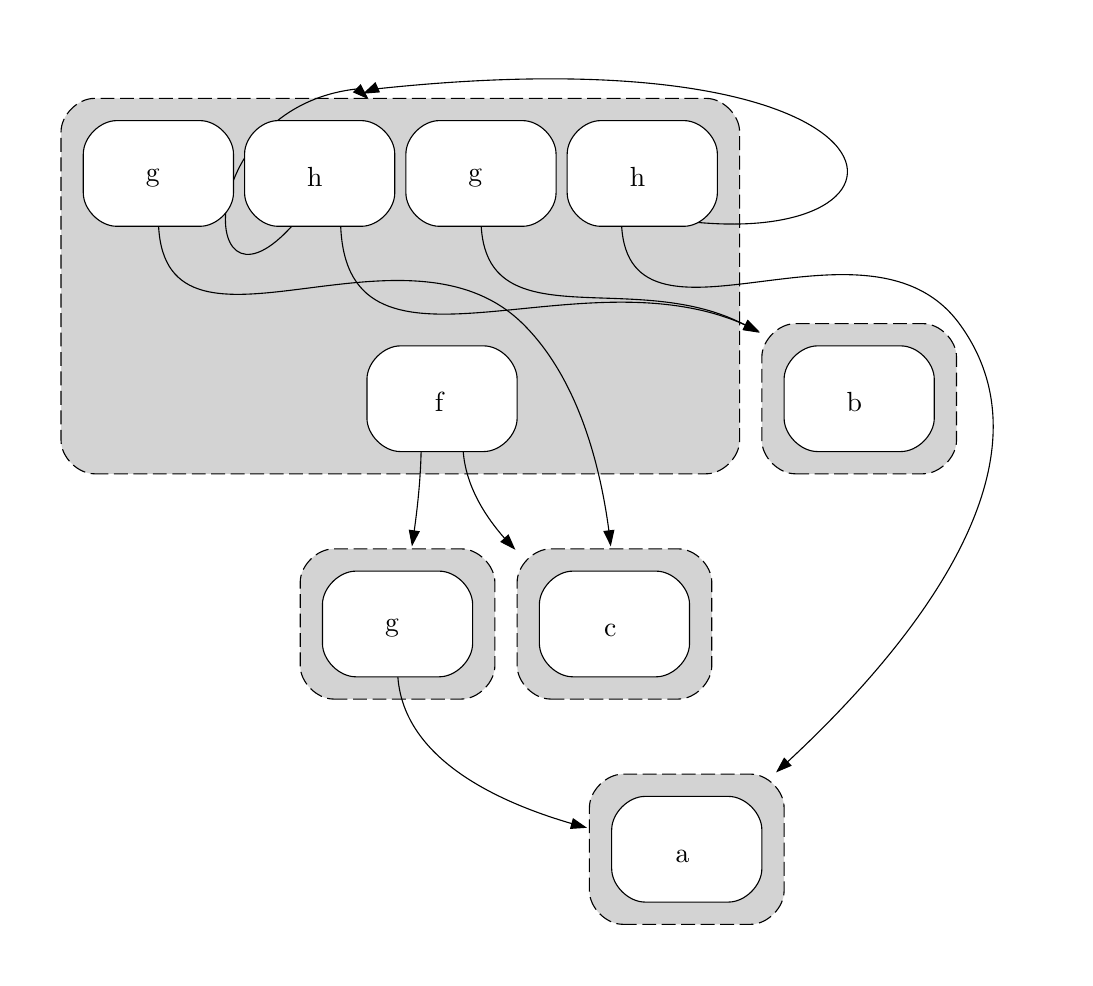
\begin{tikzpicture}[y=1cm, x=1cm, yscale=\globalscale,xscale=\globalscale, every node/.append style={scale=\globalscale}, inner sep=0pt, outer sep=0pt]
  \begin{scope}[shift={(0.1413, -11.1958)}]
    \path[fill=white] (-0.1413, 11.1958) -- (-0.1413, 22.5328) -- (12.2765, 22.5328) -- (12.2765, 11.1958) -- (-0.1413, 11.1958) -- (-0.1413, 11.1958)-- cycle;;



    \path[draw=black,fill=lightgrey,dash pattern=on 0.1766cm off 0.0706cm] (7.4168, 11.6196).. controls (7.4168, 11.6196) and (9.0414, 11.6196) .. (9.0414, 11.6196).. controls (9.2533, 11.6196) and (9.4652, 11.8315) .. (9.4652, 12.0434).. controls (9.4652, 12.0434) and (9.4652, 13.1029) .. (9.4652, 13.1029).. controls (9.4652, 13.3149) and (9.2533, 13.5268) .. (9.0414, 13.5268).. controls (9.0414, 13.5268) and (7.4168, 13.5268) .. (7.4168, 13.5268).. controls (7.2049, 13.5268) and (6.9929, 13.3149) .. (6.9929, 13.1029).. controls (6.9929, 13.1029) and (6.9929, 12.0434) .. (6.9929, 12.0434).. controls (6.9929, 11.8315) and (7.2049, 11.6196) .. (7.4168, 11.6196);



    \path[draw=black,fill=lightgrey,dash pattern=on 0.1766cm off 0.0706cm] (3.7437, 14.4803).. controls (3.7437, 14.4803) and (5.3683, 14.4803) .. (5.3683, 14.4803).. controls (5.5802, 14.4803) and (5.7921, 14.6923) .. (5.7921, 14.9042).. controls (5.7921, 14.9042) and (5.7921, 15.9637) .. (5.7921, 15.9637).. controls (5.7921, 16.1756) and (5.5802, 16.3875) .. (5.3683, 16.3875).. controls (5.3683, 16.3875) and (3.7437, 16.3875) .. (3.7437, 16.3875).. controls (3.5318, 16.3875) and (3.3199, 16.1756) .. (3.3199, 15.9637).. controls (3.3199, 15.9637) and (3.3199, 14.9042) .. (3.3199, 14.9042).. controls (3.3199, 14.6923) and (3.5318, 14.4803) .. (3.7437, 14.4803);



    \path[draw=black,fill=lightgrey,dash pattern=on 0.1766cm off 0.0706cm] (6.4985, 14.4803).. controls (6.4985, 14.4803) and (8.1231, 14.4803) .. (8.1231, 14.4803).. controls (8.335, 14.4803) and (8.5469, 14.6923) .. (8.5469, 14.9042).. controls (8.5469, 14.9042) and (8.5469, 15.9637) .. (8.5469, 15.9637).. controls (8.5469, 16.1756) and (8.335, 16.3875) .. (8.1231, 16.3875).. controls (8.1231, 16.3875) and (6.4985, 16.3875) .. (6.4985, 16.3875).. controls (6.2866, 16.3875) and (6.0747, 16.1756) .. (6.0747, 15.9637).. controls (6.0747, 15.9637) and (6.0747, 14.9042) .. (6.0747, 14.9042).. controls (6.0747, 14.6923) and (6.2866, 14.4803) .. (6.4985, 14.4803);



    \path[draw=black,fill=lightgrey,dash pattern=on 0.1766cm off 0.0706cm] (9.6065, 17.3411).. controls (9.6065, 17.3411) and (11.2311, 17.3411) .. (11.2311, 17.3411).. controls (11.443, 17.3411) and (11.6549, 17.553) .. (11.6549, 17.7649).. controls (11.6549, 17.7649) and (11.6549, 18.8244) .. (11.6549, 18.8244).. controls (11.6549, 19.0364) and (11.443, 19.2483) .. (11.2311, 19.2483).. controls (11.2311, 19.2483) and (9.6065, 19.2483) .. (9.6065, 19.2483).. controls (9.3946, 19.2483) and (9.1827, 19.0364) .. (9.1827, 18.8244).. controls (9.1827, 18.8244) and (9.1827, 17.7649) .. (9.1827, 17.7649).. controls (9.1827, 17.553) and (9.3946, 17.3411) .. (9.6065, 17.3411);



    \path[draw=black,fill=lightgrey,dash pattern=on 0.1766cm off 0.0706cm] (0.7064, 17.3411).. controls (0.7064, 17.3411) and (8.4763, 17.3411) .. (8.4763, 17.3411).. controls (8.6882, 17.3411) and (8.9001, 17.553) .. (8.9001, 17.7649).. controls (8.9001, 17.7649) and (8.9001, 21.6852) .. (8.9001, 21.6852).. controls (8.9001, 21.8971) and (8.6882, 22.109) .. (8.4763, 22.109).. controls (8.4763, 22.109) and (0.7064, 22.109) .. (0.7064, 22.109).. controls (0.4945, 22.109) and (0.2825, 21.8971) .. (0.2825, 21.6852).. controls (0.2825, 21.6852) and (0.2825, 17.7649) .. (0.2825, 17.7649).. controls (0.2825, 17.553) and (0.4945, 17.3411) .. (0.7064, 17.3411);



    \path[draw=black] (4.556, 14.8688).. controls (4.556, 13.7758) and (5.7505, 13.1944) .. (6.7772, 12.8963);



    \path[draw=black,fill=black] (6.7877, 12.9578) -- (6.9414, 12.8511) -- (6.7549, 12.8384) -- (6.7877, 12.9578) -- (6.7877, 12.9578)-- cycle;;



    \path[draw=black] (4.8562, 17.7296).. controls (4.8562, 17.3619) and (4.8167, 16.9635) .. (4.7662, 16.6047);



    \path[draw=black,fill=black] (4.829, 16.6058) -- (4.7418, 16.4405) -- (4.7068, 16.6241) -- (4.829, 16.6058) -- (4.829, 16.6058)-- cycle;;



    \path[draw=black] (5.386, 17.7296).. controls (5.386, 17.2715) and (5.618, 16.859) .. (5.921, 16.5157);



    \path[draw=black,fill=black] (5.962, 16.5623) -- (6.038, 16.3914) -- (5.872, 16.4776) -- (5.962, 16.5623) -- (5.962, 16.5623)-- cycle;;



    \path[draw=black] (1.5187, 20.5903).. controls (1.5187, 18.4494) and (4.6185, 20.7493) .. (6.1453, 19.2483).. controls (6.8481, 18.5571) and (7.1293, 17.4527) .. (7.2405, 16.6157);



    \path[draw=black,fill=black] (7.302, 16.6231) -- (7.2614, 16.4405) -- (7.1791, 16.6086) -- (7.302, 16.6231) -- (7.302, 16.6231)-- cycle;;



    \path[draw=black] (5.6155, 20.5903).. controls (5.6155, 18.9989) and (7.516, 19.968) .. (8.9354, 19.2483).. controls (8.9506, 19.2405) and (8.9662, 19.2327) .. (8.9813, 19.2246);



    \path[draw=black,fill=black] (9.0092, 19.2797) -- (9.1357, 19.142) -- (8.951, 19.1709) -- (9.0092, 19.2797) -- (9.0092, 19.2797)-- cycle;;



    \path[draw=black] (7.3991, 20.5903).. controls (7.3991, 18.5921) and (10.5067, 20.8584) .. (11.6902, 19.2483).. controls (13.0217, 17.4368) and (10.9743, 15.0423) .. (9.5058, 13.6797);



    \path[draw=black,fill=black] (9.5503, 13.6362) -- (9.3783, 13.5628) -- (9.467, 13.7277) -- (9.5503, 13.6362) -- (9.5503, 13.6362)-- cycle;;



    \path[draw=black] (7.9289, 20.5903).. controls (11.5, 20) and (11.5, 23) .. (4.2908, 22.23);



    \path[draw=black,fill=black] (4.323, 22.1913) -- (4.1361, 22.1765) -- (4.2728, 22.3043) -- (4.323, 22.1913) -- (4.323, 22.1913)-- cycle;;



    \path[draw=black] (3.832, 20.5903).. controls (3.832, 18.2449) and (6.7807, 20.1739) .. (8.9354, 19.2483).. controls (8.951, 19.2416) and (8.9662, 19.2348) .. (8.9817, 19.2281);



    \path[draw=black,fill=black] (9.0018, 19.2868) -- (9.1346, 19.1547) -- (8.9485, 19.1755) -- (9.0018, 19.2868) -- (9.0018, 19.2868)-- cycle;;



    \path[draw=black] (3.3022, 20.5903).. controls (2, 19) and (1.9, 22) .. (4.05, 22.23);



    \path[draw=black,fill=black] (4.0856, 22.2787) -- (4.1725, 22.113) -- (4.0012, 22.1883) -- (4.0856, 22.2787) -- (4.0856, 22.2787)-- cycle;;



    \path[draw=black,fill=white] (8.7588, 13.2442).. controls (8.7588, 13.2442) and (7.6993, 13.2442) .. (7.6993, 13.2442).. controls (7.4874, 13.2442) and (7.2755, 13.0323) .. (7.2755, 12.8204).. controls (7.2755, 12.8204) and (7.2755, 12.326) .. (7.2755, 12.326).. controls (7.2755, 12.114) and (7.4874, 11.9021) .. (7.6993, 11.9021).. controls (7.6993, 11.9021) and (8.7588, 11.9021) .. (8.7588, 11.9021).. controls (8.9707, 11.9021) and (9.1827, 12.114) .. (9.1827, 12.326).. controls (9.1827, 12.326) and (9.1827, 12.8204) .. (9.1827, 12.8204).. controls (9.1827, 13.0323) and (8.9707, 13.2442) .. (8.7588, 13.2442);



    \node[anchor=south west] (text857) at (8.0836, 12.4079){a};



    \path[draw=black,fill=white] (5.0858, 16.105).. controls (5.0858, 16.105) and (4.0262, 16.105) .. (4.0262, 16.105).. controls (3.8143, 16.105) and (3.6024, 15.8931) .. (3.6024, 15.6812).. controls (3.6024, 15.6812) and (3.6024, 15.1867) .. (3.6024, 15.1867).. controls (3.6024, 14.9748) and (3.8143, 14.7629) .. (4.0262, 14.7629).. controls (4.0262, 14.7629) and (5.0858, 14.7629) .. (5.0858, 14.7629).. controls (5.2977, 14.7629) and (5.5096, 14.9748) .. (5.5096, 15.1867).. controls (5.5096, 15.1867) and (5.5096, 15.6812) .. (5.5096, 15.6812).. controls (5.5096, 15.8931) and (5.2977, 16.105) .. (5.0858, 16.105);



    \node[anchor=south west] (text3101) at (4.3971, 15.269){g};



    \path[draw=black,fill=white] (7.8406, 16.105).. controls (7.8406, 16.105) and (6.781, 16.105) .. (6.781, 16.105).. controls (6.5691, 16.105) and (6.3572, 15.8931) .. (6.3572, 15.6812).. controls (6.3572, 15.6812) and (6.3572, 15.1867) .. (6.3572, 15.1867).. controls (6.3572, 14.9748) and (6.5691, 14.7629) .. (6.781, 14.7629).. controls (6.781, 14.7629) and (7.8406, 14.7629) .. (7.8406, 14.7629).. controls (8.0525, 14.7629) and (8.2644, 14.9748) .. (8.2644, 15.1867).. controls (8.2644, 15.1867) and (8.2644, 15.6812) .. (8.2644, 15.6812).. controls (8.2644, 15.8931) and (8.0525, 16.105) .. (7.8406, 16.105);



    \node[anchor=south west] (text3219) at (7.1784, 15.269){c};



    \path[draw=black,fill=white] (10.9486, 18.9657).. controls (10.9486, 18.9657) and (9.889, 18.9657) .. (9.889, 18.9657).. controls (9.6771, 18.9657) and (9.4652, 18.7538) .. (9.4652, 18.5419).. controls (9.4652, 18.5419) and (9.4652, 18.0475) .. (9.4652, 18.0475).. controls (9.4652, 17.8355) and (9.6771, 17.6236) .. (9.889, 17.6236).. controls (9.889, 17.6236) and (10.9486, 17.6236) .. (10.9486, 17.6236).. controls (11.1605, 17.6236) and (11.3724, 17.8355) .. (11.3724, 18.0475).. controls (11.3724, 18.0475) and (11.3724, 18.5419) .. (11.3724, 18.5419).. controls (11.3724, 18.7538) and (11.1605, 18.9657) .. (10.9486, 18.9657);



    \node[anchor=south west] (text7886) at (10.2599, 18.1294){b};



    \path[draw=black,fill=white] (5.6509, 18.9657).. controls (5.6509, 18.9657) and (4.5913, 18.9657) .. (4.5913, 18.9657).. controls (4.3794, 18.9657) and (4.1675, 18.7538) .. (4.1675, 18.5419).. controls (4.1675, 18.5419) and (4.1675, 18.0475) .. (4.1675, 18.0475).. controls (4.1675, 17.8355) and (4.3794, 17.6236) .. (4.5913, 17.6236).. controls (4.5913, 17.6236) and (5.6509, 17.6236) .. (5.6509, 17.6236).. controls (5.8628, 17.6236) and (6.0747, 17.8355) .. (6.0747, 18.0475).. controls (6.0747, 18.0475) and (6.0747, 18.5419) .. (6.0747, 18.5419).. controls (6.0747, 18.7538) and (5.8628, 18.9657) .. (5.6509, 18.9657);



    \node[anchor=south west] (text4244) at (5.0286, 18.1294){f};



    \path[draw=black,fill=white] (2.0484, 21.8265).. controls (2.0484, 21.8265) and (0.9889, 21.8265) .. (0.9889, 21.8265).. controls (0.777, 21.8265) and (0.5651, 21.6146) .. (0.5651, 21.4027).. controls (0.5651, 21.4027) and (0.5651, 20.9082) .. (0.5651, 20.9082).. controls (0.5651, 20.6963) and (0.777, 20.4844) .. (0.9889, 20.4844).. controls (0.9889, 20.4844) and (2.0484, 20.4844) .. (2.0484, 20.4844).. controls (2.2603, 20.4844) and (2.4723, 20.6963) .. (2.4723, 20.9082).. controls (2.4723, 20.9082) and (2.4723, 21.4027) .. (2.4723, 21.4027).. controls (2.4723, 21.6146) and (2.2603, 21.8265) .. (2.0484, 21.8265);



    \node[anchor=south west] (text214) at (1.3597, 20.9901){g};



    \path[draw=black,fill=white] (6.1453, 21.8265).. controls (6.1453, 21.8265) and (5.0858, 21.8265) .. (5.0858, 21.8265).. controls (4.8739, 21.8265) and (4.662, 21.6146) .. (4.662, 21.4027).. controls (4.662, 21.4027) and (4.662, 20.9082) .. (4.662, 20.9082).. controls (4.662, 20.6963) and (4.8739, 20.4844) .. (5.0858, 20.4844).. controls (5.0858, 20.4844) and (6.1453, 20.4844) .. (6.1453, 20.4844).. controls (6.3572, 20.4844) and (6.5691, 20.6963) .. (6.5691, 20.9082).. controls (6.5691, 20.9082) and (6.5691, 21.4027) .. (6.5691, 21.4027).. controls (6.5691, 21.6146) and (6.3572, 21.8265) .. (6.1453, 21.8265);



    \node[anchor=south west] (text1482) at (5.4566, 20.9901){g};



    \path[draw=black,fill=white] (8.1938, 21.8265).. controls (8.1938, 21.8265) and (7.1342, 21.8265) .. (7.1342, 21.8265).. controls (6.9223, 21.8265) and (6.7104, 21.6146) .. (6.7104, 21.4027).. controls (6.7104, 21.4027) and (6.7104, 20.9082) .. (6.7104, 20.9082).. controls (6.7104, 20.6963) and (6.9223, 20.4844) .. (7.1342, 20.4844).. controls (7.1342, 20.4844) and (8.1938, 20.4844) .. (8.1938, 20.4844).. controls (8.4057, 20.4844) and (8.6176, 20.6963) .. (8.6176, 20.9082).. controls (8.6176, 20.9082) and (8.6176, 21.4027) .. (8.6176, 21.4027).. controls (8.6176, 21.6146) and (8.4057, 21.8265) .. (8.1938, 21.8265);



    \node[anchor=south west] (text8602) at (7.5051, 20.9901){h};



    \path[draw=black,fill=white] (4.0969, 21.8265).. controls (4.0969, 21.8265) and (3.0373, 21.8265) .. (3.0373, 21.8265).. controls (2.8254, 21.8265) and (2.6135, 21.6146) .. (2.6135, 21.4027).. controls (2.6135, 21.4027) and (2.6135, 20.9082) .. (2.6135, 20.9082).. controls (2.6135, 20.6963) and (2.8254, 20.4844) .. (3.0373, 20.4844).. controls (3.0373, 20.4844) and (4.0969, 20.4844) .. (4.0969, 20.4844).. controls (4.3088, 20.4844) and (4.5207, 20.6963) .. (4.5207, 20.9082).. controls (4.5207, 20.9082) and (4.5207, 21.4027) .. (4.5207, 21.4027).. controls (4.5207, 21.6146) and (4.3088, 21.8265) .. (4.0969, 21.8265);



    \node[anchor=south west] (text4033) at (3.4082, 20.9901){h};



  \end{scope}

\end{tikzpicture}
\label{exampleBasic7}
\end{center}

Handling congruence closure in E-graphs with cycles is not difficult: we can just propagate until nothing changes. There is a finite upper bound on propagation: at most, we could discover that every E-node is equal to every other. Every step moves closer to that bound by merging some E-nodes. Thus, this fix-point algorithm clearly terminates.

\subsubsection{Equality saturation}
Suppose instead of the equations $h(g(c), b) = h(a, g(c))$ in the above example we had the identity $\forall x.\; h(a, x) = h(x, b)$. To do equality saturation with this identity, we would \emph{match} the left-hand-side $h(a, x)$ against our E-graph, which would find the match $h(a, g(b))$, corresponding to the substitution $x = g(b)$. Then, we apply the same substitution to the right hand side, thus finding the \emph{equations} $h(a, g(b)) = h(g(b), b)$. Inserting this equation into our E-graph and using congruence closure would then yield the above E-graph.

Equalities are symmetric, so we need to match the right-hand-side and add the substituted left-hand-side in general equality saturation.

So, in general, to handle identities, we use the following procedure:

\begin{enumerate}
\item Add every ground equation to the E-graph
\item Saturation loop:
	\begin{enumerate}
		\item (E-match) Match any side of an identity to a ground term represented by the E-graph
		\item (Propagate) Add both sides of the identity, appropriately substituted, as a new ground equation to the E-graph.
		\item Repeat
	\end{enumerate}
\end{enumerate}

\chapter{Egraphs modulo AC} \label{acegg}
One common pair of identities we want to work with is associativity

\begin{equation}
	\label{assocdef} \forall x y z.\; f(x, f(y, z)) = f(f(x, y), z)
\end{equation}

and commutativity

\begin{equation}
	\label{commdef} \forall x y.\; f(x, y) = f(y, x)
\end{equation}

We refer to this combination as AC

A common AC operator is +, and we will use that as a generic name for an AC operator.

Unfortunately, equality saturation handles these identities rather poorly. Consider as a simple case the terms of length $n$ over some constant terms $k_n$ $t_n = a + (b + (...k_n))$. Then we can see that there is a significant blowup in the size of the saturated graph as we increase $n$:

\begin{center}
	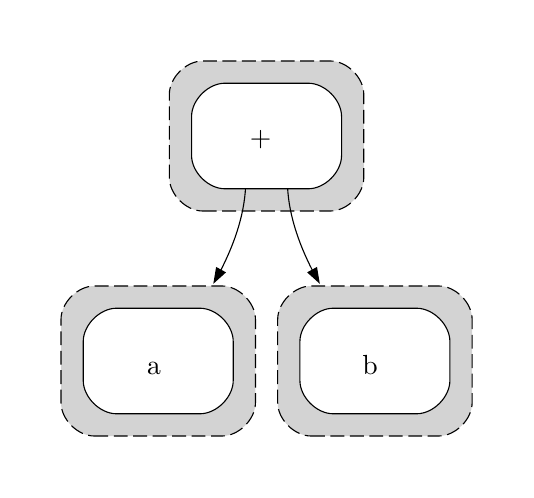
\begin{tikzpicture}[y=1cm, x=1cm, yscale=\globalscale,xscale=\globalscale, every node/.append style={scale=\globalscale}, inner sep=0pt, outer sep=0pt]
  \begin{scope}[shift={(0.1411, -5.4681)}]
    \path[fill=white] (-0.1411, 5.4681) -- (-0.1411, 11.0772) -- (5.9267, 11.0772) -- (5.9267, 5.4681) -- (-0.1411, 5.4681) -- (-0.1411, 5.4681)-- cycle;;



    \path[draw=black,fill=lightgrey,dash pattern=on 0.1764cm off 0.0706cm] (0.7056, 5.8914).. controls (0.7056, 5.8914) and (2.3283, 5.8914) .. (2.3283, 5.8914).. controls (2.54, 5.8914) and (2.7517, 6.1031) .. (2.7517, 6.3147).. controls (2.7517, 6.3147) and (2.7517, 7.3731) .. (2.7517, 7.3731).. controls (2.7517, 7.5847) and (2.54, 7.7964) .. (2.3283, 7.7964).. controls (2.3283, 7.7964) and (0.7056, 7.7964) .. (0.7056, 7.7964).. controls (0.4939, 7.7964) and (0.2822, 7.5847) .. (0.2822, 7.3731).. controls (0.2822, 7.3731) and (0.2822, 6.3147) .. (0.2822, 6.3147).. controls (0.2822, 6.1031) and (0.4939, 5.8914) .. (0.7056, 5.8914);



    \path[draw=black,fill=lightgrey,dash pattern=on 0.1764cm off 0.0706cm] (3.4572, 5.8914).. controls (3.4572, 5.8914) and (5.08, 5.8914) .. (5.08, 5.8914).. controls (5.2917, 5.8914) and (5.5033, 6.1031) .. (5.5033, 6.3147).. controls (5.5033, 6.3147) and (5.5033, 7.3731) .. (5.5033, 7.3731).. controls (5.5033, 7.5847) and (5.2917, 7.7964) .. (5.08, 7.7964).. controls (5.08, 7.7964) and (3.4572, 7.7964) .. (3.4572, 7.7964).. controls (3.2456, 7.7964) and (3.0339, 7.5847) .. (3.0339, 7.3731).. controls (3.0339, 7.3731) and (3.0339, 6.3147) .. (3.0339, 6.3147).. controls (3.0339, 6.1031) and (3.2456, 5.8914) .. (3.4572, 5.8914);



    \path[draw=black,fill=lightgrey,dash pattern=on 0.1764cm off 0.0706cm] (2.0814, 8.7489).. controls (2.0814, 8.7489) and (3.7042, 8.7489) .. (3.7042, 8.7489).. controls (3.9158, 8.7489) and (4.1275, 8.9606) .. (4.1275, 9.1722).. controls (4.1275, 9.1722) and (4.1275, 10.2306) .. (4.1275, 10.2306).. controls (4.1275, 10.4422) and (3.9158, 10.6539) .. (3.7042, 10.6539).. controls (3.7042, 10.6539) and (2.0814, 10.6539) .. (2.0814, 10.6539).. controls (1.8697, 10.6539) and (1.6581, 10.4422) .. (1.6581, 10.2306).. controls (1.6581, 10.2306) and (1.6581, 9.1722) .. (1.6581, 9.1722).. controls (1.6581, 8.9606) and (1.8697, 8.7489) .. (2.0814, 8.7489);



    \path[draw=black] (2.6282, 9.1369).. controls (2.6282, 8.7422) and (2.4899, 8.3446) .. (2.3107, 7.9957);



    \path[draw=black,fill=black] (2.3657, 7.9682) -- (2.2267, 7.843) -- (2.2574, 8.0275) -- (2.3657, 7.9682) -- (2.3657, 7.9682)-- cycle;;



    \path[draw=black] (3.1574, 9.1369).. controls (3.1574, 8.7422) and (3.2957, 8.3446) .. (3.4749, 7.9957);



    \path[draw=black,fill=black] (3.5281, 8.0275) -- (3.5588, 7.843) -- (3.4198, 7.9682) -- (3.5281, 8.0275) -- (3.5281, 8.0275)-- cycle;;



    \path[draw=black,fill=white] (2.0461, 7.5142).. controls (2.0461, 7.5142) and (0.9878, 7.5142) .. (0.9878, 7.5142).. controls (0.7761, 7.5142) and (0.5644, 7.3025) .. (0.5644, 7.0908).. controls (0.5644, 7.0908) and (0.5644, 6.5969) .. (0.5644, 6.5969).. controls (0.5644, 6.3853) and (0.7761, 6.1736) .. (0.9878, 6.1736).. controls (0.9878, 6.1736) and (2.0461, 6.1736) .. (2.0461, 6.1736).. controls (2.2578, 6.1736) and (2.4694, 6.3853) .. (2.4694, 6.5969).. controls (2.4694, 6.5969) and (2.4694, 7.0908) .. (2.4694, 7.0908).. controls (2.4694, 7.3025) and (2.2578, 7.5142) .. (2.0461, 7.5142);



    \node[anchor=south west] (text16) at (1.3716, 6.6788){a};



    \path[draw=black,fill=white] (4.7978, 7.5142).. controls (4.7978, 7.5142) and (3.7394, 7.5142) .. (3.7394, 7.5142).. controls (3.5278, 7.5142) and (3.3161, 7.3025) .. (3.3161, 7.0908).. controls (3.3161, 7.0908) and (3.3161, 6.5969) .. (3.3161, 6.5969).. controls (3.3161, 6.3853) and (3.5278, 6.1736) .. (3.7394, 6.1736).. controls (3.7394, 6.1736) and (4.7978, 6.1736) .. (4.7978, 6.1736).. controls (5.0094, 6.1736) and (5.2211, 6.3853) .. (5.2211, 6.5969).. controls (5.2211, 6.5969) and (5.2211, 7.0908) .. (5.2211, 7.0908).. controls (5.2211, 7.3025) and (5.0094, 7.5142) .. (4.7978, 7.5142);



    \node[anchor=south west] (text5380) at (4.1099, 6.6788){b};



    \path[draw=black,fill=white] (3.4219, 10.3717).. controls (3.4219, 10.3717) and (2.3636, 10.3717) .. (2.3636, 10.3717).. controls (2.1519, 10.3717) and (1.9403, 10.16) .. (1.9403, 9.9483).. controls (1.9403, 9.9483) and (1.9403, 9.4544) .. (1.9403, 9.4544).. controls (1.9403, 9.2428) and (2.1519, 9.0311) .. (2.3636, 9.0311).. controls (2.3636, 9.0311) and (3.4219, 9.0311) .. (3.4219, 9.0311).. controls (3.6336, 9.0311) and (3.8453, 9.2428) .. (3.8453, 9.4544).. controls (3.8453, 9.4544) and (3.8453, 9.9483) .. (3.8453, 9.9483).. controls (3.8453, 10.16) and (3.6336, 10.3717) .. (3.4219, 10.3717);



    \node[anchor=south west] (text5981) at (2.6811, 9.5366){+};



  \end{scope}

\end{tikzpicture}
	\label{blowup2}
\end{center}

\begin{center}
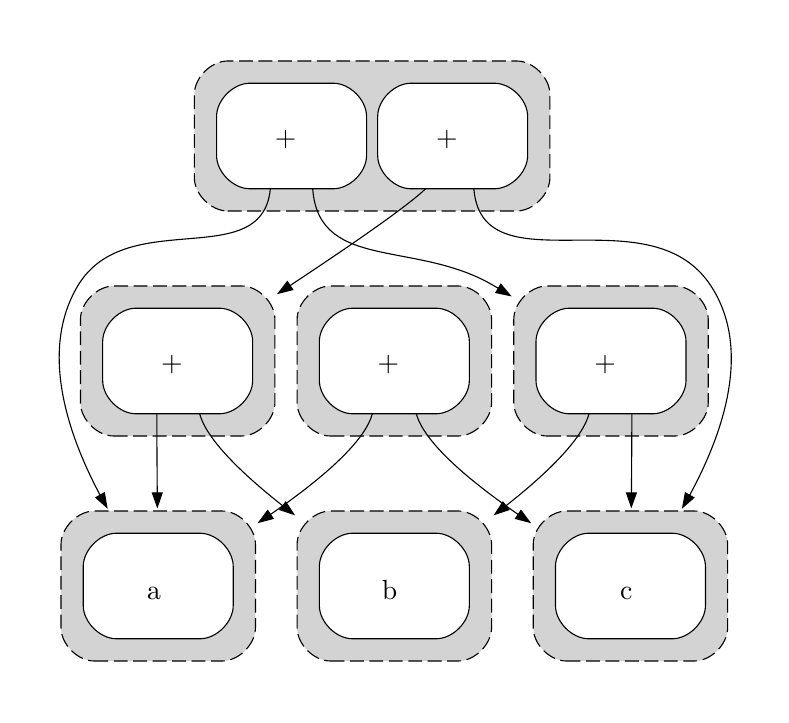
\begin{tikzpicture}[y=1cm, x=1cm, yscale=\globalscale,xscale=\globalscale, every node/.append style={scale=\globalscale}, inner sep=0pt, outer sep=0pt]
  \begin{scope}[shift={(0.1411, -8.3256)}]
    \path[fill=white] (-0.1411, 8.3256) -- (-0.1411, 16.7922) -- (9.1722, 16.7922) -- (9.1722, 8.3256) -- (-0.1411, 8.3256) -- (-0.1411, 8.3256)-- cycle;;



    \path[draw=black,fill=lightgrey,dash pattern=on 0.1764cm off 0.0706cm] (0.7056, 8.7489).. controls (0.7056, 8.7489) and (2.3283, 8.7489) .. (2.3283, 8.7489).. controls (2.54, 8.7489) and (2.7517, 8.9606) .. (2.7517, 9.1722).. controls (2.7517, 9.1722) and (2.7517, 10.2306) .. (2.7517, 10.2306).. controls (2.7517, 10.4422) and (2.54, 10.6539) .. (2.3283, 10.6539).. controls (2.3283, 10.6539) and (0.7056, 10.6539) .. (0.7056, 10.6539).. controls (0.4939, 10.6539) and (0.2822, 10.4422) .. (0.2822, 10.2306).. controls (0.2822, 10.2306) and (0.2822, 9.1722) .. (0.2822, 9.1722).. controls (0.2822, 8.9606) and (0.4939, 8.7489) .. (0.7056, 8.7489);



    \path[draw=black,fill=lightgrey,dash pattern=on 0.1764cm off 0.0706cm] (3.7042, 8.7489).. controls (3.7042, 8.7489) and (5.3269, 8.7489) .. (5.3269, 8.7489).. controls (5.5386, 8.7489) and (5.7503, 8.9606) .. (5.7503, 9.1722).. controls (5.7503, 9.1722) and (5.7503, 10.2306) .. (5.7503, 10.2306).. controls (5.7503, 10.4422) and (5.5386, 10.6539) .. (5.3269, 10.6539).. controls (5.3269, 10.6539) and (3.7042, 10.6539) .. (3.7042, 10.6539).. controls (3.4925, 10.6539) and (3.2808, 10.4422) .. (3.2808, 10.2306).. controls (3.2808, 10.2306) and (3.2808, 9.1722) .. (3.2808, 9.1722).. controls (3.2808, 8.9606) and (3.4925, 8.7489) .. (3.7042, 8.7489);



    \path[draw=black,fill=lightgrey,dash pattern=on 0.1764cm off 0.0706cm] (6.7028, 8.7489).. controls (6.7028, 8.7489) and (8.3256, 8.7489) .. (8.3256, 8.7489).. controls (8.5372, 8.7489) and (8.7489, 8.9606) .. (8.7489, 9.1722).. controls (8.7489, 9.1722) and (8.7489, 10.2306) .. (8.7489, 10.2306).. controls (8.7489, 10.4422) and (8.5372, 10.6539) .. (8.3256, 10.6539).. controls (8.3256, 10.6539) and (6.7028, 10.6539) .. (6.7028, 10.6539).. controls (6.4911, 10.6539) and (6.2794, 10.4422) .. (6.2794, 10.2306).. controls (6.2794, 10.2306) and (6.2794, 9.1722) .. (6.2794, 9.1722).. controls (6.2794, 8.9606) and (6.4911, 8.7489) .. (6.7028, 8.7489);



    \path[draw=black,fill=lightgrey,dash pattern=on 0.1764cm off 0.0706cm] (0.9525, 11.6064).. controls (0.9525, 11.6064) and (2.5753, 11.6064) .. (2.5753, 11.6064).. controls (2.7869, 11.6064) and (2.9986, 11.8181) .. (2.9986, 12.0297).. controls (2.9986, 12.0297) and (2.9986, 13.0881) .. (2.9986, 13.0881).. controls (2.9986, 13.2997) and (2.7869, 13.5114) .. (2.5753, 13.5114).. controls (2.5753, 13.5114) and (0.9525, 13.5114) .. (0.9525, 13.5114).. controls (0.7408, 13.5114) and (0.5292, 13.2997) .. (0.5292, 13.0881).. controls (0.5292, 13.0881) and (0.5292, 12.0297) .. (0.5292, 12.0297).. controls (0.5292, 11.8181) and (0.7408, 11.6064) .. (0.9525, 11.6064);



    \path[draw=black,fill=lightgrey,dash pattern=on 0.1764cm off 0.0706cm] (3.7042, 11.6064).. controls (3.7042, 11.6064) and (5.3269, 11.6064) .. (5.3269, 11.6064).. controls (5.5386, 11.6064) and (5.7503, 11.8181) .. (5.7503, 12.0297).. controls (5.7503, 12.0297) and (5.7503, 13.0881) .. (5.7503, 13.0881).. controls (5.7503, 13.2997) and (5.5386, 13.5114) .. (5.3269, 13.5114).. controls (5.3269, 13.5114) and (3.7042, 13.5114) .. (3.7042, 13.5114).. controls (3.4925, 13.5114) and (3.2808, 13.2997) .. (3.2808, 13.0881).. controls (3.2808, 13.0881) and (3.2808, 12.0297) .. (3.2808, 12.0297).. controls (3.2808, 11.8181) and (3.4925, 11.6064) .. (3.7042, 11.6064);



    \path[draw=black,fill=lightgrey,dash pattern=on 0.1764cm off 0.0706cm] (6.4558, 11.6064).. controls (6.4558, 11.6064) and (8.0786, 11.6064) .. (8.0786, 11.6064).. controls (8.2903, 11.6064) and (8.5019, 11.8181) .. (8.5019, 12.0297).. controls (8.5019, 12.0297) and (8.5019, 13.0881) .. (8.5019, 13.0881).. controls (8.5019, 13.2997) and (8.2903, 13.5114) .. (8.0786, 13.5114).. controls (8.0786, 13.5114) and (6.4558, 13.5114) .. (6.4558, 13.5114).. controls (6.2442, 13.5114) and (6.0325, 13.2997) .. (6.0325, 13.0881).. controls (6.0325, 13.0881) and (6.0325, 12.0297) .. (6.0325, 12.0297).. controls (6.0325, 11.8181) and (6.2442, 11.6064) .. (6.4558, 11.6064);



    \path[draw=black,fill=lightgrey,dash pattern=on 0.1764cm off 0.0706cm] (2.3989, 14.4639).. controls (2.3989, 14.4639) and (6.0678, 14.4639) .. (6.0678, 14.4639).. controls (6.2794, 14.4639) and (6.4911, 14.6756) .. (6.4911, 14.8872).. controls (6.4911, 14.8872) and (6.4911, 15.9456) .. (6.4911, 15.9456).. controls (6.4911, 16.1572) and (6.2794, 16.3689) .. (6.0678, 16.3689).. controls (6.0678, 16.3689) and (2.3989, 16.3689) .. (2.3989, 16.3689).. controls (2.1872, 16.3689) and (1.9756, 16.1572) .. (1.9756, 15.9456).. controls (1.9756, 15.9456) and (1.9756, 14.8872) .. (1.9756, 14.8872).. controls (1.9756, 14.6756) and (2.1872, 14.4639) .. (2.3989, 14.4639);



    \path[draw=black] (1.4993, 11.9944).. controls (1.4993, 11.6325) and (1.5014, 11.2381) .. (1.5046, 10.8818);



    \path[draw=black,fill=black] (1.5663, 10.8839) -- (1.506, 10.7072) -- (1.4429, 10.8828) -- (1.5663, 10.8839) -- (1.5663, 10.8839)-- cycle;;



    \path[draw=black] (2.0285, 11.9944).. controls (2.0285, 11.6547) and (2.5439, 11.1562) .. (3.1055, 10.7142);



    \path[draw=black,fill=black] (3.1365, 10.7682) -- (3.2385, 10.6116) -- (3.0614, 10.6705) -- (3.1365, 10.7682) -- (3.1365, 10.7682)-- cycle;;



    \path[draw=black] (4.251, 11.9944).. controls (4.251, 11.611) and (3.6036, 11.0663) .. (2.939, 10.6077);



    \path[draw=black,fill=black] (2.9764, 10.5586) -- (2.7958, 10.511) -- (2.9072, 10.6609) -- (2.9764, 10.5586) -- (2.9764, 10.5586)-- cycle;;



    \path[draw=black] (4.7801, 11.9944).. controls (4.7801, 11.611) and (5.4275, 11.0663) .. (6.0921, 10.6077);



    \path[draw=black,fill=black] (6.1239, 10.6609) -- (6.2353, 10.511) -- (6.0547, 10.5586) -- (6.1239, 10.6609) -- (6.1239, 10.6609)-- cycle;;



    \path[draw=black] (7.0026, 11.9944).. controls (7.0026, 11.6547) and (6.4872, 11.1562) .. (5.9256, 10.7142);



    \path[draw=black,fill=black] (5.9697, 10.6705) -- (5.7926, 10.6116) -- (5.8946, 10.7682) -- (5.9697, 10.6705) -- (5.9697, 10.6705)-- cycle;;



    \path[draw=black] (7.5318, 11.9944).. controls (7.5318, 11.6325) and (7.5297, 11.2381) .. (7.5265, 10.8818);



    \path[draw=black,fill=black] (7.5882, 10.8828) -- (7.5251, 10.7072) -- (7.4648, 10.8839) -- (7.5882, 10.8828) -- (7.5882, 10.8828)-- cycle;;



    \path[draw=black] (2.9457, 14.8519).. controls (2.9457, 13.6102) and (1.1275, 14.5796) .. (0.4939, 13.5114).. controls (0.0074, 12.6908) and (0.363, 11.6343) .. (0.7828, 10.8476);



    \path[draw=black,fill=black] (0.8329, 10.8846) -- (0.8647, 10.7005) -- (0.725, 10.8246) -- (0.8329, 10.8846) -- (0.8329, 10.8846)-- cycle;;



    \path[draw=black] (3.4749, 14.8519).. controls (3.4749, 13.6645) and (4.7671, 14.1217) .. (5.7856, 13.5114).. controls (5.8057, 13.4994) and (5.8261, 13.487) .. (5.8466, 13.4747);



    \path[draw=black,fill=black] (5.8681, 13.534) -- (5.987, 13.3897) -- (5.8043, 13.4281) -- (5.8681, 13.534) -- (5.8681, 13.534)-- cycle;;



    \path[draw=black] (5.521, 14.8519).. controls (5.521, 13.3851) and (7.7378, 14.7415) .. (8.5372, 13.5114).. controls (9.0593, 12.7081) and (8.6949, 11.6431) .. (8.2628, 10.8493);



    \path[draw=black,fill=black] (8.3189, 10.8232) -- (8.1781, 10.7001) -- (8.2116, 10.8843) -- (8.3189, 10.8232) -- (8.3189, 10.8232)-- cycle;;



    \path[draw=black] (4.9918, 14.8519).. controls (4.9918, 14.7338) and (4.0485, 14.0836) .. (3.1821, 13.511);



    \path[draw=black,fill=black] (3.2244, 13.4652) -- (3.0431, 13.4197) -- (3.1567, 13.5682) -- (3.2244, 13.4652) -- (3.2244, 13.4652)-- cycle;;



    \path[draw=black,fill=white] (2.0461, 10.3717).. controls (2.0461, 10.3717) and (0.9878, 10.3717) .. (0.9878, 10.3717).. controls (0.7761, 10.3717) and (0.5644, 10.16) .. (0.5644, 9.9483).. controls (0.5644, 9.9483) and (0.5644, 9.4544) .. (0.5644, 9.4544).. controls (0.5644, 9.2428) and (0.7761, 9.0311) .. (0.9878, 9.0311).. controls (0.9878, 9.0311) and (2.0461, 9.0311) .. (2.0461, 9.0311).. controls (2.2578, 9.0311) and (2.4694, 9.2428) .. (2.4694, 9.4544).. controls (2.4694, 9.4544) and (2.4694, 9.9483) .. (2.4694, 9.9483).. controls (2.4694, 10.16) and (2.2578, 10.3717) .. (2.0461, 10.3717);



    \node[anchor=south west] (text2527) at (1.3716, 9.5363){a};



    \path[draw=black,fill=white] (5.0447, 10.3717).. controls (5.0447, 10.3717) and (3.9864, 10.3717) .. (3.9864, 10.3717).. controls (3.7747, 10.3717) and (3.5631, 10.16) .. (3.5631, 9.9483).. controls (3.5631, 9.9483) and (3.5631, 9.4544) .. (3.5631, 9.4544).. controls (3.5631, 9.2428) and (3.7747, 9.0311) .. (3.9864, 9.0311).. controls (3.9864, 9.0311) and (5.0447, 9.0311) .. (5.0447, 9.0311).. controls (5.2564, 9.0311) and (5.4681, 9.2428) .. (5.4681, 9.4544).. controls (5.4681, 9.4544) and (5.4681, 9.9483) .. (5.4681, 9.9483).. controls (5.4681, 10.16) and (5.2564, 10.3717) .. (5.0447, 10.3717);



    \node[anchor=south west] (text8728) at (4.3568, 9.5363){b};



    \path[draw=black,fill=white] (8.0433, 10.3717).. controls (8.0433, 10.3717) and (6.985, 10.3717) .. (6.985, 10.3717).. controls (6.7733, 10.3717) and (6.5617, 10.16) .. (6.5617, 9.9483).. controls (6.5617, 9.9483) and (6.5617, 9.4544) .. (6.5617, 9.4544).. controls (6.5617, 9.2428) and (6.7733, 9.0311) .. (6.985, 9.0311).. controls (6.985, 9.0311) and (8.0433, 9.0311) .. (8.0433, 9.0311).. controls (8.255, 9.0311) and (8.4667, 9.2428) .. (8.4667, 9.4544).. controls (8.4667, 9.4544) and (8.4667, 9.9483) .. (8.4667, 9.9483).. controls (8.4667, 10.16) and (8.255, 10.3717) .. (8.0433, 10.3717);



    \node[anchor=south west] (text3218) at (7.3819, 9.5363){c};



    \path[draw=black,fill=white] (2.2931, 13.2292).. controls (2.2931, 13.2292) and (1.2347, 13.2292) .. (1.2347, 13.2292).. controls (1.0231, 13.2292) and (0.8114, 13.0175) .. (0.8114, 12.8058).. controls (0.8114, 12.8058) and (0.8114, 12.3119) .. (0.8114, 12.3119).. controls (0.8114, 12.1003) and (1.0231, 11.8886) .. (1.2347, 11.8886).. controls (1.2347, 11.8886) and (2.2931, 11.8886) .. (2.2931, 11.8886).. controls (2.5047, 11.8886) and (2.7164, 12.1003) .. (2.7164, 12.3119).. controls (2.7164, 12.3119) and (2.7164, 12.8058) .. (2.7164, 12.8058).. controls (2.7164, 13.0175) and (2.5047, 13.2292) .. (2.2931, 13.2292);



    \node[anchor=south west] (text4936) at (1.5522, 12.3941){+};



    \path[draw=black,fill=white] (5.0447, 13.2292).. controls (5.0447, 13.2292) and (3.9864, 13.2292) .. (3.9864, 13.2292).. controls (3.7747, 13.2292) and (3.5631, 13.0175) .. (3.5631, 12.8058).. controls (3.5631, 12.8058) and (3.5631, 12.3119) .. (3.5631, 12.3119).. controls (3.5631, 12.1003) and (3.7747, 11.8886) .. (3.9864, 11.8886).. controls (3.9864, 11.8886) and (5.0447, 11.8886) .. (5.0447, 11.8886).. controls (5.2564, 11.8886) and (5.4681, 12.1003) .. (5.4681, 12.3119).. controls (5.4681, 12.3119) and (5.4681, 12.8058) .. (5.4681, 12.8058).. controls (5.4681, 13.0175) and (5.2564, 13.2292) .. (5.0447, 13.2292);



    \node[anchor=south west] (text8548) at (4.3039, 12.3941){+};



    \path[draw=black,fill=white] (7.7964, 13.2292).. controls (7.7964, 13.2292) and (6.7381, 13.2292) .. (6.7381, 13.2292).. controls (6.5264, 13.2292) and (6.3147, 13.0175) .. (6.3147, 12.8058).. controls (6.3147, 12.8058) and (6.3147, 12.3119) .. (6.3147, 12.3119).. controls (6.3147, 12.1003) and (6.5264, 11.8886) .. (6.7381, 11.8886).. controls (6.7381, 11.8886) and (7.7964, 11.8886) .. (7.7964, 11.8886).. controls (8.0081, 11.8886) and (8.2197, 12.1003) .. (8.2197, 12.3119).. controls (8.2197, 12.3119) and (8.2197, 12.8058) .. (8.2197, 12.8058).. controls (8.2197, 13.0175) and (8.0081, 13.2292) .. (7.7964, 13.2292);



    \node[anchor=south west] (text2455) at (7.0556, 12.3941){+};



    \path[draw=black,fill=white] (3.7394, 16.0867).. controls (3.7394, 16.0867) and (2.6811, 16.0867) .. (2.6811, 16.0867).. controls (2.4694, 16.0867) and (2.2578, 15.875) .. (2.2578, 15.6633).. controls (2.2578, 15.6633) and (2.2578, 15.1694) .. (2.2578, 15.1694).. controls (2.2578, 14.9578) and (2.4694, 14.7461) .. (2.6811, 14.7461).. controls (2.6811, 14.7461) and (3.7394, 14.7461) .. (3.7394, 14.7461).. controls (3.9511, 14.7461) and (4.1628, 14.9578) .. (4.1628, 15.1694).. controls (4.1628, 15.1694) and (4.1628, 15.6633) .. (4.1628, 15.6633).. controls (4.1628, 15.875) and (3.9511, 16.0867) .. (3.7394, 16.0867);



    \node[anchor=south west] (text9837) at (2.9986, 15.2513){+};



    \path[draw=black,fill=white] (5.7856, 16.0867).. controls (5.7856, 16.0867) and (4.7272, 16.0867) .. (4.7272, 16.0867).. controls (4.5156, 16.0867) and (4.3039, 15.875) .. (4.3039, 15.6633).. controls (4.3039, 15.6633) and (4.3039, 15.1694) .. (4.3039, 15.1694).. controls (4.3039, 14.9578) and (4.5156, 14.7461) .. (4.7272, 14.7461).. controls (4.7272, 14.7461) and (5.7856, 14.7461) .. (5.7856, 14.7461).. controls (5.9972, 14.7461) and (6.2089, 14.9578) .. (6.2089, 15.1694).. controls (6.2089, 15.1694) and (6.2089, 15.6633) .. (6.2089, 15.6633).. controls (6.2089, 15.875) and (5.9972, 16.0867) .. (5.7856, 16.0867);



    \node[anchor=south west] (text5280) at (5.0447, 15.2513){+};



  \end{scope}

\end{tikzpicture}
	\label{blowup3}
\end{center}

\begin{center}
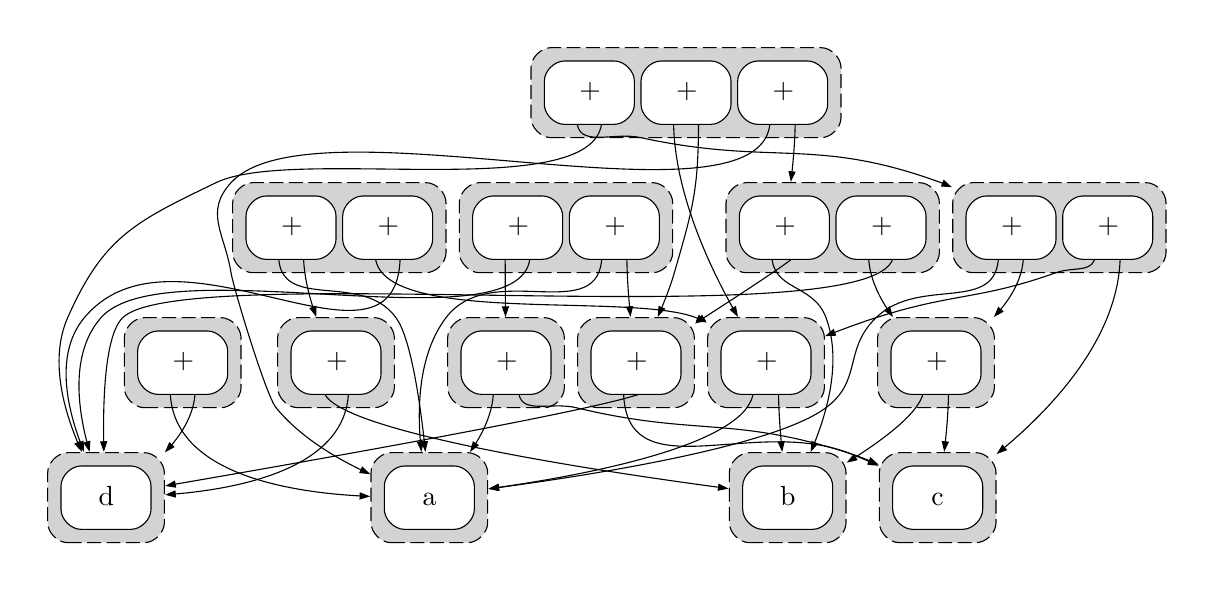
\begin{tikzpicture}[y=1cm, x=1cm, yscale=0.6,xscale=0.6, every node/.append style={scale=\globalscale}, inner sep=0pt, outer sep=0pt]
  \begin{scope}[shift={(0.1411, -11.1831)}]
    \path[fill=white] (-0.1411, 11.1831) -- (-0.1411, 22.5072) -- (24.3769, 22.5072) -- (24.3769, 11.1831) -- (-0.1411, 11.1831) -- (-0.1411, 11.1831)-- cycle;;



    \path[draw=black,fill=lightgrey,dash pattern=on 0.1764cm off 0.0706cm] (7.5494, 11.6064).. controls (7.5494, 11.6064) and (9.1722, 11.6064) .. (9.1722, 11.6064).. controls (9.3839, 11.6064) and (9.5956, 11.8181) .. (9.5956, 12.0297).. controls (9.5956, 12.0297) and (9.5956, 13.0881) .. (9.5956, 13.0881).. controls (9.5956, 13.2997) and (9.3839, 13.5114) .. (9.1722, 13.5114).. controls (9.1722, 13.5114) and (7.5494, 13.5114) .. (7.5494, 13.5114).. controls (7.3378, 13.5114) and (7.1261, 13.2997) .. (7.1261, 13.0881).. controls (7.1261, 13.0881) and (7.1261, 12.0297) .. (7.1261, 12.0297).. controls (7.1261, 11.8181) and (7.3378, 11.6064) .. (7.5494, 11.6064);



    \path[draw=black,fill=lightgrey,dash pattern=on 0.1764cm off 0.0706cm] (15.1342, 11.6064).. controls (15.1342, 11.6064) and (16.7569, 11.6064) .. (16.7569, 11.6064).. controls (16.9686, 11.6064) and (17.1803, 11.8181) .. (17.1803, 12.0297).. controls (17.1803, 12.0297) and (17.1803, 13.0881) .. (17.1803, 13.0881).. controls (17.1803, 13.2997) and (16.9686, 13.5114) .. (16.7569, 13.5114).. controls (16.7569, 13.5114) and (15.1342, 13.5114) .. (15.1342, 13.5114).. controls (14.9225, 13.5114) and (14.7108, 13.2997) .. (14.7108, 13.0881).. controls (14.7108, 13.0881) and (14.7108, 12.0297) .. (14.7108, 12.0297).. controls (14.7108, 11.8181) and (14.9225, 11.6064) .. (15.1342, 11.6064);



    \path[draw=black,fill=lightgrey,dash pattern=on 0.1764cm off 0.0706cm] (18.3092, 11.6064).. controls (18.3092, 11.6064) and (19.9319, 11.6064) .. (19.9319, 11.6064).. controls (20.1436, 11.6064) and (20.3553, 11.8181) .. (20.3553, 12.0297).. controls (20.3553, 12.0297) and (20.3553, 13.0881) .. (20.3553, 13.0881).. controls (20.3553, 13.2997) and (20.1436, 13.5114) .. (19.9319, 13.5114).. controls (19.9319, 13.5114) and (18.3092, 13.5114) .. (18.3092, 13.5114).. controls (18.0975, 13.5114) and (17.8858, 13.2997) .. (17.8858, 13.0881).. controls (17.8858, 13.0881) and (17.8858, 12.0297) .. (17.8858, 12.0297).. controls (17.8858, 11.8181) and (18.0975, 11.6064) .. (18.3092, 11.6064);



    \path[draw=black,fill=lightgrey,dash pattern=on 0.1764cm off 0.0706cm] (0.7056, 11.6064).. controls (0.7056, 11.6064) and (2.3283, 11.6064) .. (2.3283, 11.6064).. controls (2.54, 11.6064) and (2.7517, 11.8181) .. (2.7517, 12.0297).. controls (2.7517, 12.0297) and (2.7517, 13.0881) .. (2.7517, 13.0881).. controls (2.7517, 13.2997) and (2.54, 13.5114) .. (2.3283, 13.5114).. controls (2.3283, 13.5114) and (0.7056, 13.5114) .. (0.7056, 13.5114).. controls (0.4939, 13.5114) and (0.2822, 13.2997) .. (0.2822, 13.0881).. controls (0.2822, 13.0881) and (0.2822, 12.0297) .. (0.2822, 12.0297).. controls (0.2822, 11.8181) and (0.4939, 11.6064) .. (0.7056, 11.6064);



    \path[draw=black,fill=lightgrey,dash pattern=on 0.1764cm off 0.0706cm] (14.6756, 14.4639).. controls (14.6756, 14.4639) and (16.2983, 14.4639) .. (16.2983, 14.4639).. controls (16.51, 14.4639) and (16.7217, 14.6756) .. (16.7217, 14.8872).. controls (16.7217, 14.8872) and (16.7217, 15.9456) .. (16.7217, 15.9456).. controls (16.7217, 16.1572) and (16.51, 16.3689) .. (16.2983, 16.3689).. controls (16.2983, 16.3689) and (14.6756, 16.3689) .. (14.6756, 16.3689).. controls (14.4639, 16.3689) and (14.2522, 16.1572) .. (14.2522, 15.9456).. controls (14.2522, 15.9456) and (14.2522, 14.8872) .. (14.2522, 14.8872).. controls (14.2522, 14.6756) and (14.4639, 14.4639) .. (14.6756, 14.4639);



    \path[draw=black,fill=lightgrey,dash pattern=on 0.1764cm off 0.0706cm] (9.1722, 14.4639).. controls (9.1722, 14.4639) and (10.795, 14.4639) .. (10.795, 14.4639).. controls (11.0067, 14.4639) and (11.2183, 14.6756) .. (11.2183, 14.8872).. controls (11.2183, 14.8872) and (11.2183, 15.9456) .. (11.2183, 15.9456).. controls (11.2183, 16.1572) and (11.0067, 16.3689) .. (10.795, 16.3689).. controls (10.795, 16.3689) and (9.1722, 16.3689) .. (9.1722, 16.3689).. controls (8.9606, 16.3689) and (8.7489, 16.1572) .. (8.7489, 15.9456).. controls (8.7489, 15.9456) and (8.7489, 14.8872) .. (8.7489, 14.8872).. controls (8.7489, 14.6756) and (8.9606, 14.4639) .. (9.1722, 14.4639);



    \path[draw=black,fill=lightgrey,dash pattern=on 0.1764cm off 0.0706cm] (18.2739, 14.4639).. controls (18.2739, 14.4639) and (19.8967, 14.4639) .. (19.8967, 14.4639).. controls (20.1083, 14.4639) and (20.32, 14.6756) .. (20.32, 14.8872).. controls (20.32, 14.8872) and (20.32, 15.9456) .. (20.32, 15.9456).. controls (20.32, 16.1572) and (20.1083, 16.3689) .. (19.8967, 16.3689).. controls (19.8967, 16.3689) and (18.2739, 16.3689) .. (18.2739, 16.3689).. controls (18.0622, 16.3689) and (17.8506, 16.1572) .. (17.8506, 15.9456).. controls (17.8506, 15.9456) and (17.8506, 14.8872) .. (17.8506, 14.8872).. controls (17.8506, 14.6756) and (18.0622, 14.4639) .. (18.2739, 14.4639);



    \path[draw=black,fill=lightgrey,dash pattern=on 0.1764cm off 0.0706cm] (19.8614, 17.3214).. controls (19.8614, 17.3214) and (23.5303, 17.3214) .. (23.5303, 17.3214).. controls (23.7419, 17.3214) and (23.9536, 17.5331) .. (23.9536, 17.7447).. controls (23.9536, 17.7447) and (23.9536, 18.8031) .. (23.9536, 18.8031).. controls (23.9536, 19.0147) and (23.7419, 19.2264) .. (23.5303, 19.2264).. controls (23.5303, 19.2264) and (19.8614, 19.2264) .. (19.8614, 19.2264).. controls (19.6497, 19.2264) and (19.4381, 19.0147) .. (19.4381, 18.8031).. controls (19.4381, 18.8031) and (19.4381, 17.7447) .. (19.4381, 17.7447).. controls (19.4381, 17.5331) and (19.6497, 17.3214) .. (19.8614, 17.3214);



    \path[draw=black,fill=lightgrey,dash pattern=on 0.1764cm off 0.0706cm] (2.3283, 14.4639).. controls (2.3283, 14.4639) and (3.9511, 14.4639) .. (3.9511, 14.4639).. controls (4.1628, 14.4639) and (4.3744, 14.6756) .. (4.3744, 14.8872).. controls (4.3744, 14.8872) and (4.3744, 15.9456) .. (4.3744, 15.9456).. controls (4.3744, 16.1572) and (4.1628, 16.3689) .. (3.9511, 16.3689).. controls (3.9511, 16.3689) and (2.3283, 16.3689) .. (2.3283, 16.3689).. controls (2.1167, 16.3689) and (1.905, 16.1572) .. (1.905, 15.9456).. controls (1.905, 15.9456) and (1.905, 14.8872) .. (1.905, 14.8872).. controls (1.905, 14.6756) and (2.1167, 14.4639) .. (2.3283, 14.4639);



    \path[draw=black,fill=lightgrey,dash pattern=on 0.1764cm off 0.0706cm] (5.5739, 14.4639).. controls (5.5739, 14.4639) and (7.1967, 14.4639) .. (7.1967, 14.4639).. controls (7.4083, 14.4639) and (7.62, 14.6756) .. (7.62, 14.8872).. controls (7.62, 14.8872) and (7.62, 15.9456) .. (7.62, 15.9456).. controls (7.62, 16.1572) and (7.4083, 16.3689) .. (7.1967, 16.3689).. controls (7.1967, 16.3689) and (5.5739, 16.3689) .. (5.5739, 16.3689).. controls (5.3622, 16.3689) and (5.1506, 16.1572) .. (5.1506, 15.9456).. controls (5.1506, 15.9456) and (5.1506, 14.8872) .. (5.1506, 14.8872).. controls (5.1506, 14.6756) and (5.3622, 14.4639) .. (5.5739, 14.4639);



    \path[draw=black,fill=lightgrey,dash pattern=on 0.1764cm off 0.0706cm] (4.6214, 17.3214).. controls (4.6214, 17.3214) and (8.2903, 17.3214) .. (8.2903, 17.3214).. controls (8.5019, 17.3214) and (8.7136, 17.5331) .. (8.7136, 17.7447).. controls (8.7136, 17.7447) and (8.7136, 18.8031) .. (8.7136, 18.8031).. controls (8.7136, 19.0147) and (8.5019, 19.2264) .. (8.2903, 19.2264).. controls (8.2903, 19.2264) and (4.6214, 19.2264) .. (4.6214, 19.2264).. controls (4.4097, 19.2264) and (4.1981, 19.0147) .. (4.1981, 18.8031).. controls (4.1981, 18.8031) and (4.1981, 17.7447) .. (4.1981, 17.7447).. controls (4.1981, 17.5331) and (4.4097, 17.3214) .. (4.6214, 17.3214);



    \path[draw=black,fill=lightgrey,dash pattern=on 0.1764cm off 0.0706cm] (11.9239, 14.4639).. controls (11.9239, 14.4639) and (13.5467, 14.4639) .. (13.5467, 14.4639).. controls (13.7583, 14.4639) and (13.97, 14.6756) .. (13.97, 14.8872).. controls (13.97, 14.8872) and (13.97, 15.9456) .. (13.97, 15.9456).. controls (13.97, 16.1572) and (13.7583, 16.3689) .. (13.5467, 16.3689).. controls (13.5467, 16.3689) and (11.9239, 16.3689) .. (11.9239, 16.3689).. controls (11.7122, 16.3689) and (11.5006, 16.1572) .. (11.5006, 15.9456).. controls (11.5006, 15.9456) and (11.5006, 14.8872) .. (11.5006, 14.8872).. controls (11.5006, 14.6756) and (11.7122, 14.4639) .. (11.9239, 14.4639);



    \path[draw=black,fill=lightgrey,dash pattern=on 0.1764cm off 0.0706cm] (9.4192, 17.3214).. controls (9.4192, 17.3214) and (13.0881, 17.3214) .. (13.0881, 17.3214).. controls (13.2997, 17.3214) and (13.5114, 17.5331) .. (13.5114, 17.7447).. controls (13.5114, 17.7447) and (13.5114, 18.8031) .. (13.5114, 18.8031).. controls (13.5114, 19.0147) and (13.2997, 19.2264) .. (13.0881, 19.2264).. controls (13.0881, 19.2264) and (9.4192, 19.2264) .. (9.4192, 19.2264).. controls (9.2075, 19.2264) and (8.9958, 19.0147) .. (8.9958, 18.8031).. controls (8.9958, 18.8031) and (8.9958, 17.7447) .. (8.9958, 17.7447).. controls (8.9958, 17.5331) and (9.2075, 17.3214) .. (9.4192, 17.3214);



    \path[draw=black,fill=lightgrey,dash pattern=on 0.1764cm off 0.0706cm] (15.0636, 17.3214).. controls (15.0636, 17.3214) and (18.7325, 17.3214) .. (18.7325, 17.3214).. controls (18.9442, 17.3214) and (19.1558, 17.5331) .. (19.1558, 17.7447).. controls (19.1558, 17.7447) and (19.1558, 18.8031) .. (19.1558, 18.8031).. controls (19.1558, 19.0147) and (18.9442, 19.2264) .. (18.7325, 19.2264).. controls (18.7325, 19.2264) and (15.0636, 19.2264) .. (15.0636, 19.2264).. controls (14.8519, 19.2264) and (14.6403, 19.0147) .. (14.6403, 18.8031).. controls (14.6403, 18.8031) and (14.6403, 17.7447) .. (14.6403, 17.7447).. controls (14.6403, 17.5331) and (14.8519, 17.3214) .. (15.0636, 17.3214);



    \path[draw=black,fill=lightgrey,dash pattern=on 0.1764cm off 0.0706cm] (10.9361, 20.1789).. controls (10.9361, 20.1789) and (16.6511, 20.1789) .. (16.6511, 20.1789).. controls (16.8628, 20.1789) and (17.0744, 20.3906) .. (17.0744, 20.6022).. controls (17.0744, 20.6022) and (17.0744, 21.6606) .. (17.0744, 21.6606).. controls (17.0744, 21.8722) and (16.8628, 22.0839) .. (16.6511, 22.0839).. controls (16.6511, 22.0839) and (10.9361, 22.0839) .. (10.9361, 22.0839).. controls (10.7244, 22.0839) and (10.5128, 21.8722) .. (10.5128, 21.6606).. controls (10.5128, 21.6606) and (10.5128, 20.6022) .. (10.5128, 20.6022).. controls (10.5128, 20.3906) and (10.7244, 20.1789) .. (10.9361, 20.1789);



    \path[draw=black] (15.2224, 14.8519).. controls (15.2224, 13.7245) and (11.8368, 13.0669) .. (9.822, 12.7755);



    \path[draw=black,fill=black] (9.8316, 12.7145) -- (9.6481, 12.7508) -- (9.8143, 12.8365) -- (9.8316, 12.7145) -- (9.8316, 12.7145)-- cycle;;



    \path[draw=black] (15.7515, 14.8519).. controls (15.7515, 14.4893) and (15.7766, 14.0952) .. (15.809, 13.7389);



    \path[draw=black,fill=black] (15.8701, 13.746) -- (15.8256, 13.5643) -- (15.7473, 13.734) -- (15.8701, 13.746) -- (15.8701, 13.746)-- cycle;;



    \path[draw=black] (9.719, 14.8519).. controls (9.719, 14.4427) and (9.5532, 14.0437) .. (9.3373, 13.6977);



    \path[draw=black,fill=black] (9.3917, 13.6684) -- (9.2424, 13.5558) -- (9.289, 13.7368) -- (9.3917, 13.6684) -- (9.3917, 13.6684)-- cycle;;



    \path[draw=black] (10.2482, 14.8519).. controls (10.2482, 14.2843) and (10.9132, 14.5969) .. (11.4653, 14.4639).. controls (13.9838, 13.8571) and (14.7458, 14.2928) .. (17.2156, 13.5114).. controls (17.3683, 13.4631) and (17.5242, 13.4045) .. (17.678, 13.3406);



    \path[draw=black,fill=black] (17.6996, 13.3989) -- (17.8368, 13.2719) -- (17.6505, 13.2853) -- (17.6996, 13.3989) -- (17.6996, 13.3989)-- cycle;;



    \path[draw=black] (18.8207, 14.8519).. controls (18.8207, 14.4438) and (18.0954, 13.8762) .. (17.3732, 13.4119);



    \path[draw=black,fill=black] (17.4075, 13.3608) -- (17.2254, 13.3188) -- (17.3415, 13.4652) -- (17.4075, 13.3608) -- (17.4075, 13.3608)-- cycle;;



    \path[draw=black] (19.3499, 14.8519).. controls (19.3499, 14.4889) and (19.3202, 14.0949) .. (19.2821, 13.7389);



    \path[draw=black,fill=black] (19.3435, 13.7326) -- (19.2624, 13.5643) -- (19.2207, 13.7467) -- (19.3435, 13.7326) -- (19.3435, 13.7326)-- cycle;;



    \path[draw=black] (20.4082, 17.7094).. controls (20.4082, 16.4123) and (18.7463, 17.2724) .. (17.8153, 16.3689).. controls (17.1203, 15.6944) and (17.5331, 15.0435) .. (16.7569, 14.4639).. controls (15.6736, 13.655) and (11.9214, 13.0549) .. (9.8185, 12.773);



    \path[draw=black,fill=black] (9.8312, 12.7123) -- (9.6485, 12.7504) -- (9.815, 12.8348) -- (9.8312, 12.7123) -- (9.8312, 12.7123)-- cycle;;



    \path[draw=black] (20.9374, 17.7094).. controls (20.9374, 17.2731) and (20.7282, 16.8751) .. (20.4502, 16.5389);



    \path[draw=black,fill=black] (20.4982, 16.4998) -- (20.3348, 16.4088) -- (20.4057, 16.5816) -- (20.4982, 16.4998) -- (20.4982, 16.4998)-- cycle;;



    \path[draw=black] (22.9835, 17.7094).. controls (22.9835, 16.0256) and (21.6337, 14.545) .. (20.5299, 13.6158);



    \path[draw=black,fill=black] (20.5715, 13.5703) -- (20.3962, 13.5054) -- (20.4932, 13.6656) -- (20.5715, 13.5703) -- (20.5715, 13.5703)-- cycle;;



    \path[draw=black] (22.4543, 17.7094).. controls (22.4543, 17.3027) and (22.0087, 17.4576) .. (21.6253, 17.3214).. controls (19.9806, 16.7372) and (19.4776, 16.9016) .. (17.8153, 16.3689).. controls (17.5232, 16.2754) and (17.2149, 16.1636) .. (16.9217, 16.0507);



    \path[draw=black,fill=black] (16.958, 15.9985) -- (16.7714, 15.9921) -- (16.9132, 16.1135) -- (16.958, 15.9985) -- (16.958, 15.9985)-- cycle;;



    \path[draw=black] (2.8751, 14.8519).. controls (2.8751, 13.1071) and (5.2772, 12.6831) .. (6.9025, 12.5956);



    \path[draw=black,fill=black] (6.8996, 12.6573) -- (7.0728, 12.5878) -- (6.894, 12.5342) -- (6.8996, 12.6573) -- (6.8996, 12.6573)-- cycle;;



    \path[draw=black] (3.4043, 14.8519).. controls (3.4043, 14.4113) and (3.1898, 14.0113) .. (2.9058, 13.6744);



    \path[draw=black,fill=black] (2.9517, 13.6331) -- (2.7873, 13.5438) -- (2.86, 13.716) -- (2.9517, 13.6331) -- (2.9517, 13.6331)-- cycle;;



    \path[draw=black] (6.1207, 14.8519).. controls (6.1207, 14.0039) and (11.751, 13.1459) .. (14.4872, 12.779);



    \path[draw=black,fill=black] (14.4914, 12.8408) -- (14.6579, 12.7564) -- (14.4748, 12.7183) -- (14.4914, 12.8408) -- (14.4914, 12.8408)-- cycle;;



    \path[draw=black] (6.6499, 14.8519).. controls (6.6499, 13.238) and (4.4972, 12.7674) .. (2.9799, 12.6365);



    \path[draw=black,fill=black] (2.9856, 12.5748) -- (2.8049, 12.6227) -- (2.976, 12.6979) -- (2.9856, 12.5748) -- (2.9856, 12.5748)-- cycle;;



    \path[draw=black] (5.1682, 17.7094).. controls (5.1682, 16.4536) and (6.9148, 17.3831) .. (7.6553, 16.3689).. controls (7.9562, 15.9568) and (8.1495, 14.6879) .. (8.2564, 13.734);



    \path[draw=black,fill=black] (8.3171, 13.7463) -- (8.2748, 13.5643) -- (8.1943, 13.7333) -- (8.3171, 13.7463) -- (8.3171, 13.7463)-- cycle;;



    \path[draw=black] (5.6974, 17.7094).. controls (5.6974, 17.3334) and (5.7856, 16.9372) .. (5.8991, 16.583);



    \path[draw=black,fill=black] (5.9563, 16.6063) -- (5.9552, 16.4193) -- (5.8395, 16.5661) -- (5.9563, 16.6063) -- (5.9563, 16.6063)-- cycle;;



    \path[draw=black] (7.7435, 17.7094).. controls (7.7435, 14.6791) and (3.0036, 18.6926) .. (1.0583, 16.3689).. controls (0.4491, 15.6411) and (0.6689, 14.5401) .. (0.9786, 13.7146);



    \path[draw=black,fill=black] (1.0319, 13.7478) -- (1.0393, 13.5608) -- (0.9172, 13.7022) -- (1.0319, 13.7478) -- (1.0319, 13.7478)-- cycle;;



    \path[draw=black] (7.2143, 17.7094).. controls (7.2143, 16.1713) and (12.5712, 16.9259) .. (14.0053, 16.3689).. controls (14.0208, 16.3629) and (14.036, 16.3569) .. (14.0515, 16.3505);



    \path[draw=black,fill=black] (14.0677, 16.4109) -- (14.2035, 16.2825) -- (14.0173, 16.298) -- (14.0677, 16.4109) -- (14.0677, 16.4109)-- cycle;;



    \path[draw=black] (12.4707, 14.8519).. controls (12.4707, 12.6605) and (15.1663, 14.2875) .. (17.2156, 13.5114).. controls (17.3669, 13.4539) and (17.5228, 13.3893) .. (17.677, 13.3212);



    \path[draw=black,fill=black] (17.702, 13.3777) -- (17.8372, 13.2489) -- (17.6509, 13.2652) -- (17.702, 13.3777) -- (17.702, 13.3777)-- cycle;;



    \path[draw=black] (12.9999, 14.8519).. controls (12.9999, 14.5994) and (6.0688, 13.3766) .. (2.9764, 12.8436);



    \path[draw=black,fill=black] (2.9884, 12.7829) -- (2.8042, 12.8139) -- (2.9676, 12.9046) -- (2.9884, 12.7829) -- (2.9884, 12.7829)-- cycle;;



    \path[draw=black] (12.0121, 17.7094).. controls (12.0121, 16.1269) and (9.6686, 17.6308) .. (8.7136, 16.3689).. controls (8.1502, 15.6249) and (8.103, 14.5468) .. (8.1725, 13.7333);



    \path[draw=black,fill=black] (8.2331, 13.746) -- (8.1897, 13.5643) -- (8.1104, 13.7336) -- (8.2331, 13.746) -- (8.2331, 13.746)-- cycle;;



    \path[draw=black] (12.5413, 17.7094).. controls (12.5413, 17.3468) and (12.5663, 16.9527) .. (12.5988, 16.5964);



    \path[draw=black,fill=black] (12.6598, 16.6035) -- (12.6153, 16.4218) -- (12.537, 16.5915) -- (12.6598, 16.6035) -- (12.6598, 16.6035)-- cycle;;



    \path[draw=black] (10.4951, 17.7094).. controls (10.4951, 15.669) and (2.758, 17.9017) .. (1.4111, 16.3689).. controls (0.7892, 15.6612) and (0.8989, 14.5584) .. (1.1148, 13.7273);



    \path[draw=black,fill=black] (1.1726, 13.7492) -- (1.1606, 13.5629) -- (1.0537, 13.7164) -- (1.1726, 13.7492) -- (1.1726, 13.7492)-- cycle;;



    \path[draw=black] (9.966, 17.7094).. controls (9.966, 17.3475) and (9.9681, 16.9531) .. (9.9713, 16.5968);



    \path[draw=black,fill=black] (10.033, 16.5989) -- (9.9727, 16.4222) -- (9.9095, 16.5978) -- (10.033, 16.5989) -- (10.033, 16.5989)-- cycle;;



    \path[draw=black] (15.6104, 17.7094).. controls (15.6104, 16.9256) and (16.4853, 17.1044) .. (16.7569, 16.3689).. controls (17.0759, 15.5056) and (16.819, 14.4826) .. (16.5128, 13.7192);



    \path[draw=black,fill=black] (16.5714, 13.6994) -- (16.4461, 13.5604) -- (16.4574, 13.747) -- (16.5714, 13.6994) -- (16.5714, 13.6994)-- cycle;;



    \path[draw=black] (16.1396, 17.7094).. controls (16.1396, 17.6463) and (15.0887, 16.9566) .. (14.1549, 16.3558);



    \path[draw=black,fill=black] (14.1965, 16.3093) -- (14.0148, 16.2659) -- (14.1298, 16.413) -- (14.1965, 16.3093) -- (14.1965, 16.3093)-- cycle;;



    \path[draw=black] (18.1857, 17.7094).. controls (18.1857, 15.8905) and (3.175, 17.6361) .. (1.8697, 16.3689).. controls (1.5053, 16.0151) and (1.452, 14.7154) .. (1.4672, 13.7393);



    \path[draw=black,fill=black] (1.5289, 13.7425) -- (1.4711, 13.5647) -- (1.4055, 13.7396) -- (1.5289, 13.7425) -- (1.5289, 13.7425)-- cycle;;



    \path[draw=black] (17.6565, 17.7094).. controls (17.6565, 17.297) and (17.829, 16.8984) .. (18.0541, 16.5541);



    \path[draw=black,fill=black] (18.1024, 16.5926) -- (18.1532, 16.4126) -- (18.0015, 16.5216) -- (18.1024, 16.5926) -- (18.1024, 16.5926)-- cycle;;



    \path[draw=black] (15.5751, 20.5669).. controls (15.5751, 18.0135) and (5.8854, 21.1113) .. (4.1628, 19.2264).. controls (3.5916, 18.6016) and (4.0273, 18.1571) .. (4.1628, 17.3214).. controls (4.2164, 16.9912) and (4.9036, 14.7232) .. (5.1153, 14.4639).. controls (5.5908, 13.8818) and (6.2988, 13.444) .. (6.9324, 13.1389);



    \path[draw=black,fill=black] (6.9441, 13.2017) -- (7.0778, 13.0711) -- (6.8919, 13.0898) -- (6.9441, 13.2017) -- (6.9441, 13.2017)-- cycle;;



    \path[draw=black] (16.1043, 20.5669).. controls (16.1043, 20.2039) and (16.0747, 19.8099) .. (16.0366, 19.4539);



    \path[draw=black,fill=black] (16.098, 19.4476) -- (16.0168, 19.2793) -- (15.9752, 19.4617) -- (16.098, 19.4476) -- (16.098, 19.4476)-- cycle;;



    \path[draw=black] (13.529, 20.5669).. controls (13.529, 19.1121) and (14.2286, 17.5687) .. (14.7913, 16.5626);



    \path[draw=black,fill=black] (14.8417, 16.5989) -- (14.8752, 16.4151) -- (14.7345, 16.5379) -- (14.8417, 16.5989) -- (14.8417, 16.5989)-- cycle;;



    \path[draw=black] (14.0582, 20.5669).. controls (14.0582, 19.1068) and (13.9541, 18.7237) .. (13.5467, 17.3214).. controls (13.4743, 17.0723) and (13.377, 16.813) .. (13.2747, 16.5693);



    \path[draw=black,fill=black] (13.3361, 16.5555) -- (13.2094, 16.4179) -- (13.2228, 16.6042) -- (13.3361, 16.5555) -- (13.3361, 16.5555)-- cycle;;



    \path[draw=black] (12.0121, 20.5669).. controls (12.0121, 18.7279) and (5.5009, 20.0272) .. (3.8453, 19.2264).. controls (2.1467, 18.4048) and (1.4683, 18.0947) .. (0.7056, 16.3689).. controls (0.3316, 15.5229) and (0.5965, 14.4918) .. (0.9204, 13.7213);



    \path[draw=black,fill=black] (0.9768, 13.7463) -- (0.9913, 13.5601) -- (0.864, 13.6966) -- (0.9768, 13.7463) -- (0.9768, 13.7463)-- cycle;;



    \path[draw=black] (11.4829, 20.5669).. controls (11.4829, 19.939) and (12.2276, 20.3119) .. (12.8411, 20.1789).. controls (15.6302, 19.5739) and (16.5118, 20.2092) .. (19.1911, 19.2264).. controls (19.2066, 19.2207) and (19.2222, 19.2147) .. (19.2373, 19.2088);



    \path[draw=black,fill=black] (19.2514, 19.2701) -- (19.389, 19.1435) -- (19.2028, 19.1565) -- (19.2514, 19.2701) -- (19.2514, 19.2701)-- cycle;;



    \path[draw=black,fill=white] (8.89, 13.2292).. controls (8.89, 13.2292) and (7.8317, 13.2292) .. (7.8317, 13.2292).. controls (7.62, 13.2292) and (7.4083, 13.0175) .. (7.4083, 12.8058).. controls (7.4083, 12.8058) and (7.4083, 12.3119) .. (7.4083, 12.3119).. controls (7.4083, 12.1003) and (7.62, 11.8886) .. (7.8317, 11.8886).. controls (7.8317, 11.8886) and (8.89, 11.8886) .. (8.89, 11.8886).. controls (9.1017, 11.8886) and (9.3133, 12.1003) .. (9.3133, 12.3119).. controls (9.3133, 12.3119) and (9.3133, 12.8058) .. (9.3133, 12.8058).. controls (9.3133, 13.0175) and (9.1017, 13.2292) .. (8.89, 13.2292);



    \node[anchor=south west] (text4681) at (8.2155, 12.3938){a};



    \path[draw=black,fill=white] (16.4747, 13.2292).. controls (16.4747, 13.2292) and (15.4164, 13.2292) .. (15.4164, 13.2292).. controls (15.2047, 13.2292) and (14.9931, 13.0175) .. (14.9931, 12.8058).. controls (14.9931, 12.8058) and (14.9931, 12.3119) .. (14.9931, 12.3119).. controls (14.9931, 12.1003) and (15.2047, 11.8886) .. (15.4164, 11.8886).. controls (15.4164, 11.8886) and (16.4747, 11.8886) .. (16.4747, 11.8886).. controls (16.6864, 11.8886) and (16.8981, 12.1003) .. (16.8981, 12.3119).. controls (16.8981, 12.3119) and (16.8981, 12.8058) .. (16.8981, 12.8058).. controls (16.8981, 13.0175) and (16.6864, 13.2292) .. (16.4747, 13.2292);



    \node[anchor=south west] (text8552) at (15.7868, 12.3938){b};



    \path[draw=black,fill=white] (19.6497, 13.2292).. controls (19.6497, 13.2292) and (18.5914, 13.2292) .. (18.5914, 13.2292).. controls (18.3797, 13.2292) and (18.1681, 13.0175) .. (18.1681, 12.8058).. controls (18.1681, 12.8058) and (18.1681, 12.3119) .. (18.1681, 12.3119).. controls (18.1681, 12.1003) and (18.3797, 11.8886) .. (18.5914, 11.8886).. controls (18.5914, 11.8886) and (19.6497, 11.8886) .. (19.6497, 11.8886).. controls (19.8614, 11.8886) and (20.0731, 12.1003) .. (20.0731, 12.3119).. controls (20.0731, 12.3119) and (20.0731, 12.8058) .. (20.0731, 12.8058).. controls (20.0731, 13.0175) and (19.8614, 13.2292) .. (19.6497, 13.2292);



    \node[anchor=south west] (text9510) at (18.9883, 12.3938){c};



    \path[draw=black,fill=white] (2.0461, 13.2292).. controls (2.0461, 13.2292) and (0.9878, 13.2292) .. (0.9878, 13.2292).. controls (0.7761, 13.2292) and (0.5644, 13.0175) .. (0.5644, 12.8058).. controls (0.5644, 12.8058) and (0.5644, 12.3119) .. (0.5644, 12.3119).. controls (0.5644, 12.1003) and (0.7761, 11.8886) .. (0.9878, 11.8886).. controls (0.9878, 11.8886) and (2.0461, 11.8886) .. (2.0461, 11.8886).. controls (2.2578, 11.8886) and (2.4694, 12.1003) .. (2.4694, 12.3119).. controls (2.4694, 12.3119) and (2.4694, 12.8058) .. (2.4694, 12.8058).. controls (2.4694, 13.0175) and (2.2578, 13.2292) .. (2.0461, 13.2292);



    \node[anchor=south west] (text7270) at (1.3582, 12.3938){d};



    \path[draw=black,fill=white] (16.0161, 16.0867).. controls (16.0161, 16.0867) and (14.9578, 16.0867) .. (14.9578, 16.0867).. controls (14.7461, 16.0867) and (14.5344, 15.875) .. (14.5344, 15.6633).. controls (14.5344, 15.6633) and (14.5344, 15.1694) .. (14.5344, 15.1694).. controls (14.5344, 14.9578) and (14.7461, 14.7461) .. (14.9578, 14.7461).. controls (14.9578, 14.7461) and (16.0161, 14.7461) .. (16.0161, 14.7461).. controls (16.2278, 14.7461) and (16.4394, 14.9578) .. (16.4394, 15.1694).. controls (16.4394, 15.1694) and (16.4394, 15.6633) .. (16.4394, 15.6633).. controls (16.4394, 15.875) and (16.2278, 16.0867) .. (16.0161, 16.0867);



    \node[anchor=south west] (text8198) at (15.2753, 15.2516){+};



    \path[draw=black,fill=white] (10.5128, 16.0867).. controls (10.5128, 16.0867) and (9.4544, 16.0867) .. (9.4544, 16.0867).. controls (9.2428, 16.0867) and (9.0311, 15.875) .. (9.0311, 15.6633).. controls (9.0311, 15.6633) and (9.0311, 15.1694) .. (9.0311, 15.1694).. controls (9.0311, 14.9578) and (9.2428, 14.7461) .. (9.4544, 14.7461).. controls (9.4544, 14.7461) and (10.5128, 14.7461) .. (10.5128, 14.7461).. controls (10.7244, 14.7461) and (10.9361, 14.9578) .. (10.9361, 15.1694).. controls (10.9361, 15.1694) and (10.9361, 15.6633) .. (10.9361, 15.6633).. controls (10.9361, 15.875) and (10.7244, 16.0867) .. (10.5128, 16.0867);



    \node[anchor=south west] (text762) at (9.7719, 15.2516){+};



    \path[draw=black,fill=white] (19.6144, 16.0867).. controls (19.6144, 16.0867) and (18.5561, 16.0867) .. (18.5561, 16.0867).. controls (18.3444, 16.0867) and (18.1328, 15.875) .. (18.1328, 15.6633).. controls (18.1328, 15.6633) and (18.1328, 15.1694) .. (18.1328, 15.1694).. controls (18.1328, 14.9578) and (18.3444, 14.7461) .. (18.5561, 14.7461).. controls (18.5561, 14.7461) and (19.6144, 14.7461) .. (19.6144, 14.7461).. controls (19.8261, 14.7461) and (20.0378, 14.9578) .. (20.0378, 15.1694).. controls (20.0378, 15.1694) and (20.0378, 15.6633) .. (20.0378, 15.6633).. controls (20.0378, 15.875) and (19.8261, 16.0867) .. (19.6144, 16.0867);



    \node[anchor=south west] (text4293) at (18.8736, 15.2516){+};



    \path[draw=black,fill=white] (21.2019, 18.9442).. controls (21.2019, 18.9442) and (20.1436, 18.9442) .. (20.1436, 18.9442).. controls (19.9319, 18.9442) and (19.7203, 18.7325) .. (19.7203, 18.5208).. controls (19.7203, 18.5208) and (19.7203, 18.0269) .. (19.7203, 18.0269).. controls (19.7203, 17.8153) and (19.9319, 17.6036) .. (20.1436, 17.6036).. controls (20.1436, 17.6036) and (21.2019, 17.6036) .. (21.2019, 17.6036).. controls (21.4136, 17.6036) and (21.6253, 17.8153) .. (21.6253, 18.0269).. controls (21.6253, 18.0269) and (21.6253, 18.5208) .. (21.6253, 18.5208).. controls (21.6253, 18.7325) and (21.4136, 18.9442) .. (21.2019, 18.9442);



    \node[anchor=south west] (text9199) at (20.4611, 18.1088){+};



    \path[draw=black,fill=white] (23.2481, 18.9442).. controls (23.2481, 18.9442) and (22.1897, 18.9442) .. (22.1897, 18.9442).. controls (21.9781, 18.9442) and (21.7664, 18.7325) .. (21.7664, 18.5208).. controls (21.7664, 18.5208) and (21.7664, 18.0269) .. (21.7664, 18.0269).. controls (21.7664, 17.8153) and (21.9781, 17.6036) .. (22.1897, 17.6036).. controls (22.1897, 17.6036) and (23.2481, 17.6036) .. (23.2481, 17.6036).. controls (23.4597, 17.6036) and (23.6714, 17.8153) .. (23.6714, 18.0269).. controls (23.6714, 18.0269) and (23.6714, 18.5208) .. (23.6714, 18.5208).. controls (23.6714, 18.7325) and (23.4597, 18.9442) .. (23.2481, 18.9442);



    \node[anchor=south west] (text1438) at (22.5072, 18.1088){+};



    \path[draw=black,fill=white] (3.6689, 16.0867).. controls (3.6689, 16.0867) and (2.6106, 16.0867) .. (2.6106, 16.0867).. controls (2.3989, 16.0867) and (2.1872, 15.875) .. (2.1872, 15.6633).. controls (2.1872, 15.6633) and (2.1872, 15.1694) .. (2.1872, 15.1694).. controls (2.1872, 14.9578) and (2.3989, 14.7461) .. (2.6106, 14.7461).. controls (2.6106, 14.7461) and (3.6689, 14.7461) .. (3.6689, 14.7461).. controls (3.8806, 14.7461) and (4.0922, 14.9578) .. (4.0922, 15.1694).. controls (4.0922, 15.1694) and (4.0922, 15.6633) .. (4.0922, 15.6633).. controls (4.0922, 15.875) and (3.8806, 16.0867) .. (3.6689, 16.0867);



    \node[anchor=south west] (text3133) at (2.9281, 15.2516){+};



    \path[draw=black,fill=white] (6.9144, 16.0867).. controls (6.9144, 16.0867) and (5.8561, 16.0867) .. (5.8561, 16.0867).. controls (5.6444, 16.0867) and (5.4328, 15.875) .. (5.4328, 15.6633).. controls (5.4328, 15.6633) and (5.4328, 15.1694) .. (5.4328, 15.1694).. controls (5.4328, 14.9578) and (5.6444, 14.7461) .. (5.8561, 14.7461).. controls (5.8561, 14.7461) and (6.9144, 14.7461) .. (6.9144, 14.7461).. controls (7.1261, 14.7461) and (7.3378, 14.9578) .. (7.3378, 15.1694).. controls (7.3378, 15.1694) and (7.3378, 15.6633) .. (7.3378, 15.6633).. controls (7.3378, 15.875) and (7.1261, 16.0867) .. (6.9144, 16.0867);



    \node[anchor=south west] (text4102) at (6.1736, 15.2516){+};



    \path[draw=black,fill=white] (5.9619, 18.9442).. controls (5.9619, 18.9442) and (4.9036, 18.9442) .. (4.9036, 18.9442).. controls (4.6919, 18.9442) and (4.4803, 18.7325) .. (4.4803, 18.5208).. controls (4.4803, 18.5208) and (4.4803, 18.0269) .. (4.4803, 18.0269).. controls (4.4803, 17.8153) and (4.6919, 17.6036) .. (4.9036, 17.6036).. controls (4.9036, 17.6036) and (5.9619, 17.6036) .. (5.9619, 17.6036).. controls (6.1736, 17.6036) and (6.3853, 17.8153) .. (6.3853, 18.0269).. controls (6.3853, 18.0269) and (6.3853, 18.5208) .. (6.3853, 18.5208).. controls (6.3853, 18.7325) and (6.1736, 18.9442) .. (5.9619, 18.9442);



    \node[anchor=south west] (text9144) at (5.2211, 18.1088){+};



    \path[draw=black,fill=white] (8.0081, 18.9442).. controls (8.0081, 18.9442) and (6.9497, 18.9442) .. (6.9497, 18.9442).. controls (6.7381, 18.9442) and (6.5264, 18.7325) .. (6.5264, 18.5208).. controls (6.5264, 18.5208) and (6.5264, 18.0269) .. (6.5264, 18.0269).. controls (6.5264, 17.8153) and (6.7381, 17.6036) .. (6.9497, 17.6036).. controls (6.9497, 17.6036) and (8.0081, 17.6036) .. (8.0081, 17.6036).. controls (8.2197, 17.6036) and (8.4314, 17.8153) .. (8.4314, 18.0269).. controls (8.4314, 18.0269) and (8.4314, 18.5208) .. (8.4314, 18.5208).. controls (8.4314, 18.7325) and (8.2197, 18.9442) .. (8.0081, 18.9442);



    \node[anchor=south west] (text8934) at (7.2672, 18.1088){+};



    \path[draw=black,fill=white] (13.2644, 16.0867).. controls (13.2644, 16.0867) and (12.2061, 16.0867) .. (12.2061, 16.0867).. controls (11.9944, 16.0867) and (11.7828, 15.875) .. (11.7828, 15.6633).. controls (11.7828, 15.6633) and (11.7828, 15.1694) .. (11.7828, 15.1694).. controls (11.7828, 14.9578) and (11.9944, 14.7461) .. (12.2061, 14.7461).. controls (12.2061, 14.7461) and (13.2644, 14.7461) .. (13.2644, 14.7461).. controls (13.4761, 14.7461) and (13.6878, 14.9578) .. (13.6878, 15.1694).. controls (13.6878, 15.1694) and (13.6878, 15.6633) .. (13.6878, 15.6633).. controls (13.6878, 15.875) and (13.4761, 16.0867) .. (13.2644, 16.0867);



    \node[anchor=south west] (text8363) at (12.5236, 15.2516){+};



    \path[draw=black,fill=white] (12.8058, 18.9442).. controls (12.8058, 18.9442) and (11.7475, 18.9442) .. (11.7475, 18.9442).. controls (11.5358, 18.9442) and (11.3242, 18.7325) .. (11.3242, 18.5208).. controls (11.3242, 18.5208) and (11.3242, 18.0269) .. (11.3242, 18.0269).. controls (11.3242, 17.8153) and (11.5358, 17.6036) .. (11.7475, 17.6036).. controls (11.7475, 17.6036) and (12.8058, 17.6036) .. (12.8058, 17.6036).. controls (13.0175, 17.6036) and (13.2292, 17.8153) .. (13.2292, 18.0269).. controls (13.2292, 18.0269) and (13.2292, 18.5208) .. (13.2292, 18.5208).. controls (13.2292, 18.7325) and (13.0175, 18.9442) .. (12.8058, 18.9442);



    \node[anchor=south west] (text9979) at (12.065, 18.1088){+};



    \path[draw=black,fill=white] (10.7597, 18.9442).. controls (10.7597, 18.9442) and (9.7014, 18.9442) .. (9.7014, 18.9442).. controls (9.4897, 18.9442) and (9.2781, 18.7325) .. (9.2781, 18.5208).. controls (9.2781, 18.5208) and (9.2781, 18.0269) .. (9.2781, 18.0269).. controls (9.2781, 17.8153) and (9.4897, 17.6036) .. (9.7014, 17.6036).. controls (9.7014, 17.6036) and (10.7597, 17.6036) .. (10.7597, 17.6036).. controls (10.9714, 17.6036) and (11.1831, 17.8153) .. (11.1831, 18.0269).. controls (11.1831, 18.0269) and (11.1831, 18.5208) .. (11.1831, 18.5208).. controls (11.1831, 18.7325) and (10.9714, 18.9442) .. (10.7597, 18.9442);



    \node[anchor=south west] (text6555) at (10.0189, 18.1088){+};



    \path[draw=black,fill=white] (16.4042, 18.9442).. controls (16.4042, 18.9442) and (15.3458, 18.9442) .. (15.3458, 18.9442).. controls (15.1342, 18.9442) and (14.9225, 18.7325) .. (14.9225, 18.5208).. controls (14.9225, 18.5208) and (14.9225, 18.0269) .. (14.9225, 18.0269).. controls (14.9225, 17.8153) and (15.1342, 17.6036) .. (15.3458, 17.6036).. controls (15.3458, 17.6036) and (16.4042, 17.6036) .. (16.4042, 17.6036).. controls (16.6158, 17.6036) and (16.8275, 17.8153) .. (16.8275, 18.0269).. controls (16.8275, 18.0269) and (16.8275, 18.5208) .. (16.8275, 18.5208).. controls (16.8275, 18.7325) and (16.6158, 18.9442) .. (16.4042, 18.9442);



    \node[anchor=south west] (text2473) at (15.6633, 18.1088){+};



    \path[draw=black,fill=white] (18.4503, 18.9442).. controls (18.4503, 18.9442) and (17.3919, 18.9442) .. (17.3919, 18.9442).. controls (17.1803, 18.9442) and (16.9686, 18.7325) .. (16.9686, 18.5208).. controls (16.9686, 18.5208) and (16.9686, 18.0269) .. (16.9686, 18.0269).. controls (16.9686, 17.8153) and (17.1803, 17.6036) .. (17.3919, 17.6036).. controls (17.3919, 17.6036) and (18.4503, 17.6036) .. (18.4503, 17.6036).. controls (18.6619, 17.6036) and (18.8736, 17.8153) .. (18.8736, 18.0269).. controls (18.8736, 18.0269) and (18.8736, 18.5208) .. (18.8736, 18.5208).. controls (18.8736, 18.7325) and (18.6619, 18.9442) .. (18.4503, 18.9442);



    \node[anchor=south west] (text5836) at (17.7094, 18.1088){+};



    \path[draw=black,fill=white] (16.3689, 21.8017).. controls (16.3689, 21.8017) and (15.3106, 21.8017) .. (15.3106, 21.8017).. controls (15.0989, 21.8017) and (14.8872, 21.59) .. (14.8872, 21.3783).. controls (14.8872, 21.3783) and (14.8872, 20.8844) .. (14.8872, 20.8844).. controls (14.8872, 20.6728) and (15.0989, 20.4611) .. (15.3106, 20.4611).. controls (15.3106, 20.4611) and (16.3689, 20.4611) .. (16.3689, 20.4611).. controls (16.5806, 20.4611) and (16.7922, 20.6728) .. (16.7922, 20.8844).. controls (16.7922, 20.8844) and (16.7922, 21.3783) .. (16.7922, 21.3783).. controls (16.7922, 21.59) and (16.5806, 21.8017) .. (16.3689, 21.8017);



    \node[anchor=south west] (text9503) at (15.6281, 20.9663){+};



    \path[draw=black,fill=white] (14.3228, 21.8017).. controls (14.3228, 21.8017) and (13.2644, 21.8017) .. (13.2644, 21.8017).. controls (13.0528, 21.8017) and (12.8411, 21.59) .. (12.8411, 21.3783).. controls (12.8411, 21.3783) and (12.8411, 20.8844) .. (12.8411, 20.8844).. controls (12.8411, 20.6728) and (13.0528, 20.4611) .. (13.2644, 20.4611).. controls (13.2644, 20.4611) and (14.3228, 20.4611) .. (14.3228, 20.4611).. controls (14.5344, 20.4611) and (14.7461, 20.6728) .. (14.7461, 20.8844).. controls (14.7461, 20.8844) and (14.7461, 21.3783) .. (14.7461, 21.3783).. controls (14.7461, 21.59) and (14.5344, 21.8017) .. (14.3228, 21.8017);



    \node[anchor=south west] (text831) at (13.5819, 20.9663){+};



    \path[draw=black,fill=white] (12.2767, 21.8017).. controls (12.2767, 21.8017) and (11.2183, 21.8017) .. (11.2183, 21.8017).. controls (11.0067, 21.8017) and (10.795, 21.59) .. (10.795, 21.3783).. controls (10.795, 21.3783) and (10.795, 20.8844) .. (10.795, 20.8844).. controls (10.795, 20.6728) and (11.0067, 20.4611) .. (11.2183, 20.4611).. controls (11.2183, 20.4611) and (12.2767, 20.4611) .. (12.2767, 20.4611).. controls (12.4883, 20.4611) and (12.7, 20.6728) .. (12.7, 20.8844).. controls (12.7, 20.8844) and (12.7, 21.3783) .. (12.7, 21.3783).. controls (12.7, 21.59) and (12.4883, 21.8017) .. (12.2767, 21.8017);



    \node[anchor=south west] (text9618) at (11.5358, 20.9663){+};



  \end{scope}

\end{tikzpicture}
	\label{blowup4}
\end{center}

\begin{center}
\begin{adjustwidth}{-100pt}{-100pt}
	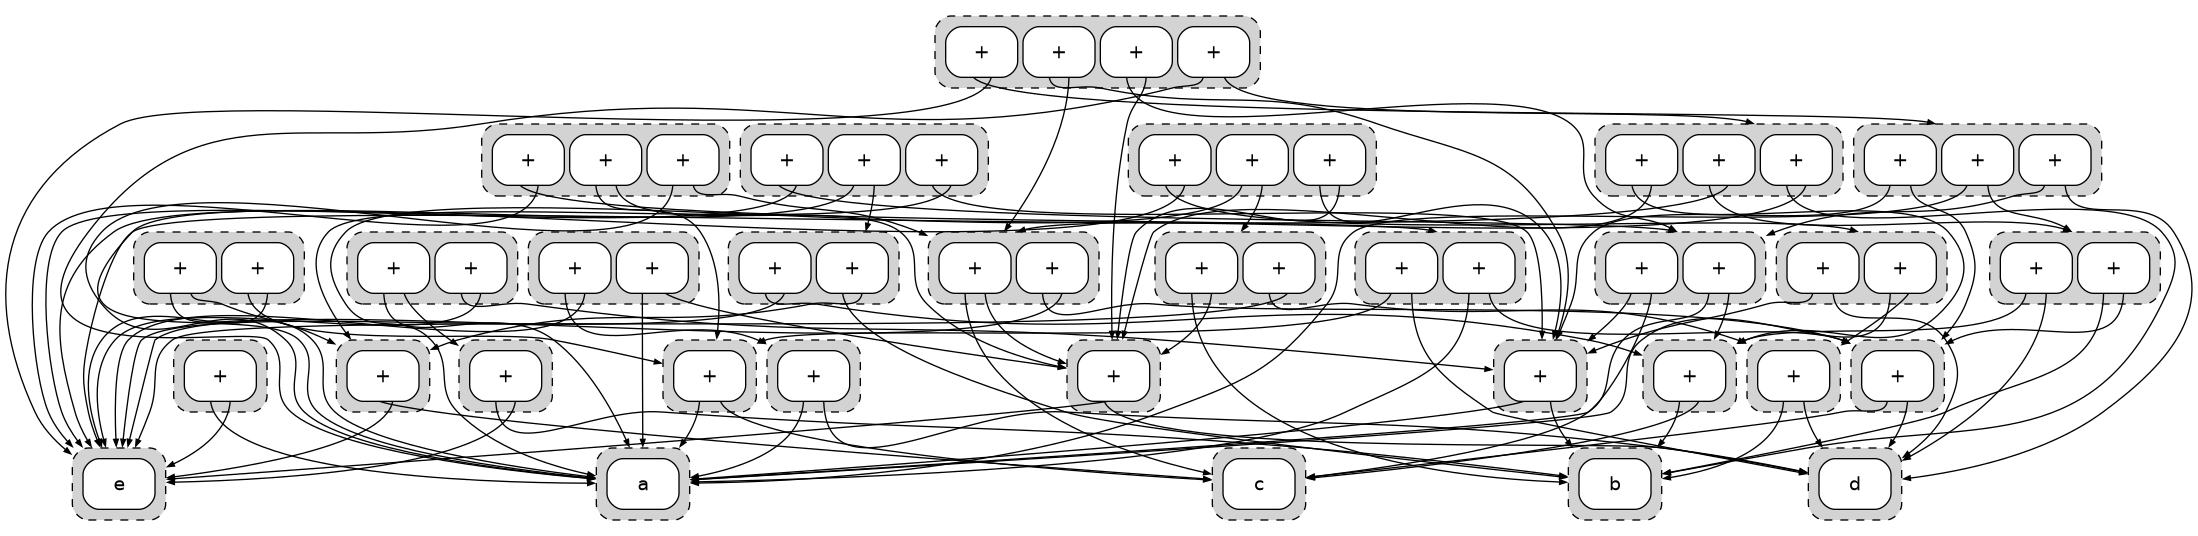
\includegraphics[scale=0.25]{blowup5.png}
\end{adjustwidth}
	\label{blowup5}
\end{center}

It's relatively easy to see why: the top E-class has $2^n-1$ E-nodes, one for each way to partition the set of atoms into 2 nonempty parts, so the E-nodes in the top class already have $2^n-1$ E-classes as children. And then each child E-class representing the sum of $k$ atoms has its own $2^k$ enodes, etc. So, there are $O(2^n)$ E-nodes for each of $O(2^n)$ E-classes, giving a doubly-exponentially sized E-graph.

\section{Handling AC with EMTs: a first example}
The difficult with plain E-graphs motivates developing a notion of \emph{E-graphs modulo theories}, where we work modulo AC (the theory we will focus on now)

We will use an example problem: besides the AC operator $+$, we introduce a function symbol $f$ and the identity $\forall xy.\; f(x + y) + 1 = f(x) + f(y)$. We also allow integer constants $k_i$, and treat integer arithmetic as an identity: $\forall xy.\; k_i + k_j = k_{i+j}$. Indeed, we will write integer constants directly.

We begin with the term $f(a) + (f(b) + f(c))$. We would like to discover that this input term is equal to $2 + f(a + (b + c))$, using the reasoning

\begin{align*}
	&f(a) + (f(b) + f(c)) = \\
	&f(a) + (f(b + c) + 1) = \\
	&(f(a) + f(b + c)) + 1 = \\
	&(f(a + (b + c)) + 1) + 1 = \\
	&f(a + (b + c)) + (1 + 1) = \\
	&f(a + (b + c)) + 2 = \\
	&2 + f(a + (b + c))
\end{align*}

We will present a pictorial overview of how we might solve the above problem using equality saturation on EMTs rather than E-graphs.

The natural first step is to simply not add any different representations of terms that are equal up to AC; thus, nodes in the E-graph for AC operators will be variadic and we will consider their children unordered. This is the key idea from prior work (\citep{zucker_omelets_2025}, \citep{panchekha_lin-graphs_2025}, \citep{shanabrook_custom_2026}).

Figure \ref{emte1} begins with the variadic AC-term $f(a) + f(b) + f(c)$.
We omit the labels of equivalence classes.

\begin{figure}[ht!]
	\centering
	\caption{EMT of the term $f(a) + f(b) + f(c)$.}
  \label{emte1}
	\begin{tikzpicture}[
			scale=2,
			transform shape,
			every node/.style={
					draw,
					fill=white!20,
					text height=1.5ex, % Height above the baseline
					text depth=0.25ex, % Depth below the baseline
					rounded corners
				}
		]
		\node (s) at (1, 3) {$+$};
		\node (f0) at (0, 1.5) {$f$};
		\node (f1) at (1, 1.5) {$f$};
		\node (f2) at (2, 1.5) {$f$};
		\node (n0) at (0, 0) {$a$};
		\node (n1) at (1, 0) {$b$};
		\node (n2) at (2, 0) {$c$};

		\begin{pgfonlayer}{background}
		\node[draw=none, fill=black!15, inner sep=12pt, fit=(n0)] (bn0) {};
		\draw[dashed, rounded corners=3pt]
		(bn0.north east) --
		(bn0.north west) --
		(bn0.south west) --
		(bn0.south east) -- cycle;

		\node[draw=none, fill=black!15, inner sep=12pt, fit=(n1)] (bn1) {};
		\draw[dashed, rounded corners=3pt]
		(bn1.north east) --
		(bn1.north west) --
		(bn1.south west) --
		(bn1.south east) -- cycle;
		
		\node[draw=none, fill=black!15, inner sep=12pt, fit=(n2)] (bn2) {};
		\draw[dashed, rounded corners=3pt]
		(bn2.north east) --
		(bn2.north west) --
		(bn2.south west) --
		(bn2.south east) -- cycle;

		\node[draw=none, fill=black!15, inner sep=12pt, fit=(f0)] (bf0) {};
		\draw[dashed, rounded corners=3pt]
		(bf0.north east) --
		(bf0.north west) --
		(bf0.south west) --
		(bf0.south east) -- cycle;

		\node[draw=none, fill=black!15, inner sep=12pt, fit=(f1)] (bf1) {};
		\draw[dashed, rounded corners=3pt]
		(bf1.north east) --
		(bf1.north west) --
		(bf1.south west) --
		(bf1.south east) -- cycle;
		
		\node[draw=none, fill=black!15, inner sep=12pt, fit=(f2)] (bf2) {};
		\draw[dashed, rounded corners=3pt]
		(bf2.north east) --
		(bf2.north west) --
		(bf2.south west) --
		(bf2.south east) -- cycle;
		
		\node[draw=none, fill=black!15, inner sep=12pt, fit=(s)] (bs) {};
		\draw[dashed, rounded corners=3pt]
		(bs.north east) --
		(bs.north west) --
		(bs.south west) --
		(bs.south east) -- cycle;
		\end{pgfonlayer}
		
		\draw[->, >=stealth, thick] (bn0.north) to[out=90, in=270, looseness=1] (bf0.south);
		\draw[->, >=stealth, thick] (bn1.north) to[out=90, in=270, looseness=1] (bf1.south);
		\draw[->, >=stealth, thick] (bn2.north) to[out=90, in=270, looseness=1] (bf2.south);
		
		\draw[->, >=stealth, thick] (bf0.north) to[out=90, in=270, looseness=1] (s.south);
		\draw[->, >=stealth, thick] (bf1.north) to[out=90, in=270, looseness=1] (s.south);
		\draw[->, >=stealth, thick] (bf2.north) to[out=90, in=270, looseness=1] (s.south);	
	\end{tikzpicture}
\end{figure}

Now, in order to \emph{match} the left-hand side of $f(x) + f(y) = f(x + y) + 1$, we need to do \emph{matching modulo theories}, which will tell us of six matches: $(x, y) \in \{(a, b), (a, c), (b, c), (b, a), (c, a), (c, b)\}$. Then we will add the six substituted forms of $f(x + y) = 1$. Here, we will want to \emph{insert modulo theories}, in a way that keeps the E-graph from representing multiple AC-equivalent terms. The arrows in Figure \ref{emte2} have become crowded, but top E-class now represents the original term, and $f(a + b) + f(c) + 1$ and its variants with $a,b,c$ permuted.

\begin{figure}[ht!]
	\centering
	\caption{EMT of the term $f(a) + f(b) + f(c)$ after some steps.}
  \label{emte2}
	\begin{tikzpicture}[
			scale=2,
			transform shape,
			every node/.style={
					draw,
					fill=white,
					text height=1.5ex, % Height above the baseline
					text depth=0.25ex, % Depth below the baseline
					rounded corners
				}
		]
		\node (s) at (0, 4.5) {$+$};
		\node (r0) at (2, 4.5) {$+$};
		\node (r1) at (3, 4.5) {$+$};
		\node (r2) at (4, 4.5) {$+$};
		\node (f0) at (0, 3) {$f$};
		\node (f1) at (1, 3) {$f$};
		\node (f2) at (2, 3) {$f$};
		\node (f01) at (3, 3) {$f$};
		\node (f02) at (4, 3) {$f$};
		\node (f12) at (5, 3) {$f$};
		\node (n01) at (3, 1.5) {$+$};
		\node (n02) at (4, 1.5) {$+$};
		\node (n12) at (5, 1.5) {$+$};
		\node (n0) at (0, 0) {$a$};
		\node (n1) at (1, 0) {$b$};
		\node (n2) at (2, 0) {$c$};
		\node (c1) at (3, 0) {$1$};

		\begin{pgfonlayer}{background}
		\node[draw=none, fill=black!15, inner sep=12pt, fit=(n0)] (bn0) {};
		\draw[dashed, rounded corners=3pt]
		(bn0.north east) --
		(bn0.north west) --
		(bn0.south west) --
		(bn0.south east) -- cycle;
		\node[draw=none, fill=black!15, inner sep=12pt, fit=(n1)] (bn1) {};
		\draw[dashed, rounded corners=3pt]
		(bn1.north east) --
		(bn1.north west) --
		(bn1.south west) --
		(bn1.south east) -- cycle;
		\node[draw=none, fill=black!15, inner sep=12pt, fit=(n2)] (bn2) {};
		\draw[dashed, rounded corners=3pt]
		(bn2.north east) --
		(bn2.north west) --
		(bn2.south west) --
		(bn2.south east) -- cycle;
		
		\node[draw=none, fill=black!15, inner sep=12pt, fit=(c1)] (bc1) {};
		\draw[dashed, rounded corners=3pt]
		(bc1.north east) --
		(bc1.north west) --
		(bc1.south west) --
		(bc1.south east) -- cycle;
		
		\node[draw=none, fill=black!15, inner sep=12pt, fit=(n01)] (bn01) {};
		\draw[dashed, rounded corners=3pt]
		(bn01.north east) --
		(bn01.north west) --
		(bn01.south west) --
		(bn01.south east) -- cycle;
		\node[draw=none, fill=black!15, inner sep=12pt, fit=(n02)] (bn02) {};
		\draw[dashed, rounded corners=3pt]
		(bn02.north east) --
		(bn02.north west) --
		(bn02.south west) --
		(bn02.south east) -- cycle;
		\node[draw=none, fill=black!15, inner sep=12pt, fit=(n12)] (bn12) {};
		\draw[dashed, rounded corners=3pt]
		(bn12.north east) --
		(bn12.north west) --
		(bn12.south west) --
		(bn12.south east) -- cycle;

		\node[draw=none, fill=black!15, inner sep=12pt, fit=(f0)] (bf0) {};
		\draw[dashed, rounded corners=3pt]
		(bf0.north east) --
		(bf0.north west) --
		(bf0.south west) --
		(bf0.south east) -- cycle;
		\node[draw=none, fill=black!15, inner sep=12pt, fit=(f1)] (bf1) {};
		\draw[dashed, rounded corners=3pt]
		(bf1.north east) --
		(bf1.north west) --
		(bf1.south west) --
		(bf1.south east) -- cycle;
		\node[draw=none, fill=black!15, inner sep=12pt, fit=(f2)] (bf2) {};
		\draw[dashed, rounded corners=3pt]
		(bf2.north east) --
		(bf2.north west) --
		(bf2.south west) --
		(bf2.south east) -- cycle;
		
		\node[draw=none, fill=black!15, inner sep=12pt, fit=(f01)] (bf01) {};
		\draw[dashed, rounded corners=3pt]
		(bf01.north east) --
		(bf01.north west) --
		(bf01.south west) --
		(bf01.south east) -- cycle;
		\node[draw=none, fill=black!15, inner sep=12pt, fit=(f02)] (bf02) {};
		\draw[dashed, rounded corners=3pt]
		(bf02.north east) --
		(bf02.north west) --
		(bf02.south west) --
		(bf02.south east) -- cycle;
		\node[draw=none, fill=black!15, inner sep=12pt, fit=(f12)] (bf12) {};
		\draw[dashed, rounded corners=3pt]
		(bf12.north east) --
		(bf12.north west) --
		(bf12.south west) --
		(bf12.south east) -- cycle;
		
		\node[draw=none, fill=black!15, inner sep=12pt, fit=(s) (r0) (r1) (r2)] (bs) {};
		\draw[dashed, rounded corners=3pt]
		(bs.north east) --
		(bs.north west) --
		(bs.south west) --
		(bs.south east) -- cycle;
		\end{pgfonlayer}
		
		\draw[->, >=stealth, thick] (bn0.north) to[out=90, in=270, looseness=1] (f0.south);
		\draw[->, >=stealth, thick] (bn1.north) to[out=90, in=270, looseness=1] (f1.south);
		\draw[->, >=stealth, thick] (bn2.north) to[out=90, in=270, looseness=1] (f2.south);
		
		\draw[->, >=stealth, thick] (bn0.north) to[out=90, in=270, looseness=1] (n01.south);
		\draw[->, >=stealth, thick] (bn1.north) to[out=90, in=270, looseness=1] (n01.south);
		\draw[->, >=stealth, thick] (bn0.north) to[out=90, in=270, looseness=1] (n02.south);
		\draw[->, >=stealth, thick] (bn2.north) to[out=90, in=270, looseness=1] (n02.south);
		\draw[->, >=stealth, thick] (bn1.north) to[out=90, in=270, looseness=1] (n12.south);
		\draw[->, >=stealth, thick] (bn2.north) to[out=90, in=270, looseness=1] (n12.south);
		
		\draw[->, >=stealth, thick] (bn01.north) to[out=90, in=270, looseness=1] (f01.south);
		\draw[->, >=stealth, thick] (bn02.north) to[out=90, in=270, looseness=1] (f02.south);
		\draw[->, >=stealth, thick] (bn12.north) to[out=90, in=270, looseness=1] (f12.south);
		
		\draw[->, >=stealth, thick] (bf0.north) to[out=90, in=270, looseness=1] (s.south);
		\draw[->, >=stealth, thick] (bf1.north) to[out=90, in=270, looseness=1] (s.south);
		\draw[->, >=stealth, thick] (bf2.north) to[out=90, in=270, looseness=1] (s.south);
		
		\draw[->, >=stealth, thick] (bf01.north) to[out=90, in=270, looseness=1] (r0.south);
		\draw[->, >=stealth, thick] (bf2.north) to[out=90, in=270, looseness=1] (r0.south);
		\draw[->, >=stealth, thick] (bc1.north) to[out=90, in=270, looseness=1]
			([xshift=0.75ex]bn12.east) to[out=90, in=270, looseness=1]
			([xshift=0.75ex]bf12.east) to[out=90, in=270, looseness=1]
			(r0.south);
		
		\draw[->, >=stealth, thick] (bf02.north) to[out=90, in=270, looseness=1] (r1.south);
		\draw[->, >=stealth, thick] (bf1.north) to[out=90, in=270, looseness=1] (r1.south);
		\draw[->, >=stealth, thick] (bc1.north) to[out=90, in=270, looseness=1] 
			([xshift=0.75ex]bn12.east) to[out=90, in=270, looseness=1]
			([xshift=0.75ex]bf12.east) to[out=90, in=270, looseness=1]
			(r1.south);
		
		\draw[->, >=stealth, thick] (bf12.north) to[out=90, in=270, looseness=1] (r2.south);
		\draw[->, >=stealth, thick] (bf0.north) to[out=90, in=270, looseness=1] (r2.south);
		\draw[->, >=stealth, thick] (bc1.north) to[out=90, in=270, looseness=1]
			([xshift=0.75ex]bn12.east) to[out=90, in=270, looseness=1]
			([xshift=0.75ex]bf12.east) to[out=90, in=270, looseness=1]
			(r2.south);
	\end{tikzpicture}
\end{figure}

Now, we once again try to match $f(x) + f(y)$. The only new matches will be $(x, y) = (a + b, c)$ and its permutations, and, modulo AC, the substituted-for term $f(x + y) + 1$ will be the same for all of these. So, we just need to add a single node.

Our last step is to notice that the term $f(a + b + c) + 1 + 1$ has, up to AC, the implicit subterm $1 + 1$, which we can reduce to $2$. Having reduced the implicit subterm, we no longer need the 3-part term $f(a + b + c) + 1 + 1$, and can entirely replace it with $f(a + b + c) + 2$.

The final EMT (Figure \ref{emte3}) is saturated, and has `discovered' our desired equality.

\begin{figure}[ht!]
	\centering
	\caption{EMT of the term $f(a) + f(b) + f(c)$ once saturated, highlighting the desired term.}
  \label{emte3}
	\begin{tikzpicture}[
			scale=2,
			transform shape,
			every node/.style={
					draw,
					fill=white,
					text height=1.5ex, % Height above the baseline
					text depth=0.25ex, % Depth below the baseline
					rounded corners
				}
		]
		\node (s) at (0, 4.5) {$+$};
		\node[fill=green!30, ultra thick] (t) at (1, 4.5) {$+$};
		\node (r0) at (2, 4.5) {$+$};
		\node (r1) at (3, 4.5) {$+$};
		\node (r2) at (4, 4.5) {$+$};
		\node (f0) at (0, 3) {$f$};
		\node (f1) at (1, 3) {$f$};
		\node (f2) at (2, 3) {$f$};
		\node[fill=green!30, ultra thick] (f012) at (3, 3) {$f$};
		\node (f01) at (4, 3) {$f$};
		\node (f02) at (5, 3) {$f$};
		\node (f12) at (6, 3) {$f$};
		\node[fill=green!30, ultra thick] (n012) at (0, 1.5) {$+$};
		\node (n01) at (1, 1.5) {$+$};
		\node (n02) at (2, 1.5) {$+$};
		\node (n12) at (3, 1.5) {$+$};
		\node (n0) at (1, 0) {$a$};
		\node (n1) at (2, 0) {$b$};
		\node (n2) at (3, 0) {$c$};
		\node[fill=green!30, ultra thick] (c2) at (4, 1.5) {$2$};
		\node (c1p1) at (5, 1.5) {$+$};
		\node (c1) at (4, 0) {$1$};

		\begin{pgfonlayer}{background}
		\node[draw=none, fill=black!15, inner sep=12pt, fit=(n0)] (bn0) {};
		\draw[dashed, rounded corners=3pt]
		(bn0.north east) --
		(bn0.north west) --
		(bn0.south west) --
		(bn0.south east) -- cycle;
		\node[draw=none, fill=black!15, inner sep=12pt, fit=(n1)] (bn1) {};
		\draw[dashed, rounded corners=3pt]
		(bn1.north east) --
		(bn1.north west) --
		(bn1.south west) --
		(bn1.south east) -- cycle;
		\node[draw=none, fill=black!15, inner sep=12pt, fit=(n2)] (bn2) {};
		\draw[dashed, rounded corners=3pt]
		(bn2.north east) --
		(bn2.north west) --
		(bn2.south west) --
		(bn2.south east) -- cycle;
		
		\node[draw=none, fill=black!15, inner sep=12pt, fit=(c1)] (bc1) {};
		\draw[dashed, rounded corners=3pt]
		(bc1.north east) --
		(bc1.north west) --
		(bc1.south west) --
		(bc1.south east) -- cycle;
		\node[draw=none, fill=black!15, inner sep=12pt, fit=(c2) (c1p1)] (bc2) {};
		\draw[dashed, rounded corners=3pt]
		(bc2.north east) --
		(bc2.north west) --
		(bc2.south west) --
		(bc2.south east) -- cycle;
		
		\node[draw=none, fill=black!15, inner sep=12pt, fit=(n01)] (bn01) {};
		\draw[dashed, rounded corners=3pt]
		(bn01.north east) --
		(bn01.north west) --
		(bn01.south west) --
		(bn01.south east) -- cycle;
		\node[draw=none, fill=black!15, inner sep=12pt, fit=(n02)] (bn02) {};
		\draw[dashed, rounded corners=3pt]
		(bn02.north east) --
		(bn02.north west) --
		(bn02.south west) --
		(bn02.south east) -- cycle;
		\node[draw=none, fill=black!15, inner sep=12pt, fit=(n12)] (bn12) {};
		\draw[dashed, rounded corners=3pt]
		(bn12.north east) --
		(bn12.north west) --
		(bn12.south west) --
		(bn12.south east) -- cycle;
		\node[draw=none, fill=black!15, inner sep=12pt, fit=(n012)] (bn012) {};
		\draw[dashed, rounded corners=3pt]
		(bn012.north east) --
		(bn012.north west) --
		(bn012.south west) --
		(bn012.south east) -- cycle;

		\node[draw=none, fill=black!15, inner sep=12pt, fit=(f0)] (bf0) {};
		\draw[dashed, rounded corners=3pt]
		(bf0.north east) --
		(bf0.north west) --
		(bf0.south west) --
		(bf0.south east) -- cycle;
		\node[draw=none, fill=black!15, inner sep=12pt, fit=(f1)] (bf1) {};
		\draw[dashed, rounded corners=3pt]
		(bf1.north east) --
		(bf1.north west) --
		(bf1.south west) --
		(bf1.south east) -- cycle;
		\node[draw=none, fill=black!15, inner sep=12pt, fit=(f2)] (bf2) {};
		\draw[dashed, rounded corners=3pt]
		(bf2.north east) --
		(bf2.north west) --
		(bf2.south west) --
		(bf2.south east) -- cycle;
		
		\node[draw=none, fill=black!15, inner sep=12pt, fit=(f012)] (bf012) {};
		\draw[dashed, rounded corners=3pt]
		(bf012.north east) --
		(bf012.north west) --
		(bf012.south west) --
		(bf012.south east) -- cycle;
		\node[draw=none, fill=black!15, inner sep=12pt, fit=(f01)] (bf01) {};
		\draw[dashed, rounded corners=3pt]
		(bf01.north east) --
		(bf01.north west) --
		(bf01.south west) --
		(bf01.south east) -- cycle;
		\node[draw=none, fill=black!15, inner sep=12pt, fit=(f02)] (bf02) {};
		\draw[dashed, rounded corners=3pt]
		(bf02.north east) --
		(bf02.north west) --
		(bf02.south west) --
		(bf02.south east) -- cycle;
		\node[draw=none, fill=black!15, inner sep=12pt, fit=(f12)] (bf12) {};
		\draw[dashed, rounded corners=3pt]
		(bf12.north east) --
		(bf12.north west) --
		(bf12.south west) --
		(bf12.south east) -- cycle;
		
		\node[draw=none, fill=black!15, inner sep=12pt, fit=(s) (t) (r0) (r1) (r2)] (bs) {};
		\draw[dashed, rounded corners=3pt]
		(bs.north east) --
		(bs.north west) --
		(bs.south west) --
		(bs.south east) -- cycle;
		\end{pgfonlayer}
		
		\draw[->, >=stealth, thick] (bn0.north) to[out=90, in=270, looseness=1] (f0.south);
		\draw[->, >=stealth, thick] (bn1.north) to[out=90, in=270, looseness=1] (f1.south);
		\draw[->, >=stealth, thick] (bn2.north) to[out=90, in=270, looseness=1] (f2.south);
		
		\draw[->, >=stealth, thick] (bn0.north) to[out=90, in=270, looseness=1] (n01.south);
		\draw[->, >=stealth, thick] (bn1.north) to[out=90, in=270, looseness=1] (n01.south);
		\draw[->, >=stealth, thick] (bn0.north) to[out=90, in=270, looseness=1] (n02.south);
		\draw[->, >=stealth, thick] (bn2.north) to[out=90, in=270, looseness=1] (n02.south);
		\draw[->, >=stealth, thick] (bn1.north) to[out=90, in=270, looseness=1] (n12.south);
		\draw[->, >=stealth, thick] (bn2.north) to[out=90, in=270, looseness=1] (n12.south);
		
		\draw[->, >=stealth, thick] (bn01.north) to[out=90, in=270, looseness=1] (f01.south);
		\draw[->, >=stealth, thick] (bn02.north) to[out=90, in=270, looseness=1] (f02.south);
		\draw[->, >=stealth, thick] (bn12.north) to[out=90, in=270, looseness=1] (f12.south);
		
		\draw[->, >=stealth, thick] (bf0.north) to[out=90, in=270, looseness=1] (s.south);
		\draw[->, >=stealth, thick] (bf1.north) to[out=90, in=270, looseness=1] (s.south);
		\draw[->, >=stealth, thick] (bf2.north) to[out=90, in=270, looseness=1] (s.south);
		
		\draw[->, >=stealth, thick] (bf01.north) to[out=90, in=270, looseness=1] (r0.south);
		\draw[->, >=stealth, thick] (bf2.north) to[out=90, in=270, looseness=1] (r0.south);
		\draw[->, >=stealth, thick] (bc1.north) to[out=90, in=270, looseness=1]
			([xshift=1.25ex]bc2.east) to[out=90, in=270, looseness=1]
			([xshift=0.75ex]bf12.east) to[out=90, in=270, looseness=1]
			(r0.south);
		
		\draw[->, >=stealth, thick] (bf02.north) to[out=90, in=270, looseness=1] (r1.south);
		\draw[->, >=stealth, thick] (bf1.north) to[out=90, in=270, looseness=1] (r1.south);
		\draw[->, >=stealth, thick] (bc1.north) to[out=90, in=270, looseness=1] 
			([xshift=1.25ex]bc2.east) to[out=90, in=270, looseness=1]
			([xshift=0.75ex]bf12.east) to[out=90, in=270, looseness=1]
			(r1.south);
		
		\draw[->, >=stealth, thick] (bf12.north) to[out=90, in=270, looseness=1] (r2.south);
		\draw[->, >=stealth, thick] (bf0.north) to[out=90, in=270, looseness=1] (r2.south);
		\draw[->, >=stealth, thick] (bc1.north) to[out=90, in=270, looseness=1]
			([xshift=1.25ex]bc2.east) to[out=90, in=270, looseness=1]
			([xshift=0.75ex]bf12.east) to[out=90, in=270, looseness=1]
			(r2.south);
			
		\draw[->, >=stealth, thick] (bc1.north) to[out=90, in=225, looseness=1] (c1p1.south);
		\draw[->, >=stealth, thick] (bc1.north) to[out=90, in=315, looseness=1] (c1p1.south);
		
		\draw[->, >=stealth, thick] (bn0.north) to[out=90, in=270, looseness=1] (n012.south);
		\draw[->, >=stealth, thick] (bn1.north) to[out=90, in=270, looseness=1] (n012.south);
		\draw[->, >=stealth, thick] (bn2.north) to[out=90, in=270, looseness=1] (n012.south);
		\draw[->, >=stealth, thick] (bn012.north) to[out=90, in=270, looseness=1] (bf012.south);
		\draw[->, >=stealth, thick] (bf012.north) to[out=90, in=270, looseness=1] (t.south);
		\draw[->, >=stealth, thick] (bc2.north) to[out=90, in=270, looseness=1] (t.south);
	\end{tikzpicture}
\end{figure}

\fxerror{Should I unfloat the preceding diagrams?}

\section{Challenges for EMT(AC)}
We have seen the promising aspects of EMTs for AC, but there is a significant gap in the description given so far, and we need something extra. Consider the equations

\begin{align}
	a + b &= b \\
	a + a &= c \\
	c + b &= d
\end{align}
taken modulo associativity of $+$.

We can represent them with an E-graph as follows:

\begin{center}
	\begin{tikzpicture}[
			scale=2,
			transform shape,
			every node/.style={
					draw,
					fill=white,
					text height=1.5ex, % Height above the baseline
					text depth=0.25ex, % Depth below the baseline
					rounded corners
				}
		]
		\node (na) at (0, 0) {$a$};
		\node (nb) at (1, 0) {$b$};
		\node (nc) at (2, 0) {$c$};
		\node (nd) at (3, 0) {$d$};
		\node (nab) at (1, 1) {$+$};
		\node (naa) at (2, 1) {$+$};
		\node (nbc) at (3, 1) {$+$};

		\node[
			draw=none,
			fill=none,
			inner sep=12pt,         % Space between nodes and the box border
			fit=(nb) (nab),     % Tells TikZ which nodes to enclose
		] (box1) {};

		\node[
			draw=none,
			fill=none,
			inner sep=12pt,         % Space between nodes and the box border
			fit=(nc) (naa),     % Tells TikZ which nodes to enclose
		] (box2) {};
		
		\node[
			draw=none,
			fill=none,
			inner sep=12pt,         % Space between nodes and the box border
			fit=(nd) (nbc),     % Tells TikZ which nodes to enclose
		] (box3) {};

		\begin{pgfonlayer}{background}
		\draw[dashed, fill=black!15, rounded corners=3pt]
		(box1.north east) --
		(box1.north west) node[midway, draw=none, fill=green!10, inner sep=1pt] {\small $e_b$} --
		(box1.south west) --
		(box1.south east) -- cycle;
		
		\draw[dashed, fill=black!15, rounded corners=3pt]
		(box2.north east) --
		(box2.north west) node[midway, draw=none, fill=green!10, inner sep=1pt] {\small $e_c$} --
		(box2.south west) --
		(box2.south east) -- cycle;
		
		\draw[dashed, fill=black!15, rounded corners=3pt]
		(box3.north east) --
		(box3.north west) node[midway, draw=none, fill=green!10, inner sep=1pt] {\small $e_d$} --
		(box3.south west) --
		(box3.south east) -- cycle;
		\end{pgfonlayer}
		
		\draw[->, >=stealth, thick] (na.north) to[out=90, in=270, looseness=1] ([xshift=-0.5em]nab.south);
		\draw[->, >=stealth, thick] (na.north) to[out=90, in=270, looseness=1] ([xshift=-0.5em]naa.south);
		\draw[->, >=stealth, thick] (na.north) to[out=90, in=270, looseness=1.2] ([xshift=0.5em]naa.south);
		\draw[->, >=stealth, thick] (box1.north) to[out=90, in=90, looseness=1]
		([yshift=0.5em]box1.east) to[out=270, in=270, looseness=1] ([xshift=0.5em]nab.south);
		\draw[->, >=stealth, thick] (box1.north) to[out=90, in=270, looseness=1] ([xshift=-0.5em]nbc.south);
		\draw[->, >=stealth, thick] (box2.north) to[out=90, in=270, looseness=1] ([xshift=0.5em]nbc.south);
		
	\end{tikzpicture}
\end{center}

Consider the equation $b = d$, which follows from the simple deduction
\begin{align*}
	b = a + b = a + (a + b) = (a + a) + b = c + b = d
\end{align*}

However, $e_b$ and $e_d$ are two distinct E-classes in the E-graph! Why?

The central step in the deduction relies on two different associations of the term $a + a + b$. The association $(a + a) + b$ is correctly assigned to class $e_d$, while the association $a + (a + b)$ is correctly assigned to the class $e_b$. However, given that we want to work modulo theories, we need to discover the fact that $e_b = e_d$, or we are throwing out some of the consequences derivable from the theory.

\section{Filling the gap}
To fill the gap, we need to reason about when such an `overlapping' term could occur, while not generating all AC-subterms like equality saturation would.

Our criteria is this: if the EMT contains two terms $t_1 = r + s$ and $t_2 = u + s$ then we need to insert the equation $t_1 + u = t_2 + r$.

This equation is a consequence, since $t_1 + u = (r + s) + u = (u + s) + r = t_2 + r$.

With our above example, we see that $e_b$ contains the E-node $+(a, e_b)$ and $e_c$ contains the E-node $+(a, a)$. Consequently, we insert the equation $e_b + a = e_c + e_b$. Since the right-hand-side is already assigned to $e_d$ and the left-hand-side to $e_b$, this equation simply asks us to equate $e_b$ and $e_d$, exactly as desired.

Let's refine the idea into something more workable. Suppose we have the variadic +-term $+(e_1, \ldots, e_k)$ in some E-class $e$, and the variadic +-term $+(d_1, \ldots, d_i)$ in some E-class $d$. Think of the arguments as multisets, so that $\{e_1, \ldots, e_k\} = E$ and similarly for $D$. Then let the multiset $O$ contain each element with the minimum multiplicity it occurs in either $E$ or $D$. So if $E = \{e_1, e_1, e_2, e_3\}$ and $D = \{e_1, e_3, e_4\}$, then $O = \{e_1, e_3\}$. If the overlap is empty, we can ignore it. Otherwise, construct the terms $E - O + D$ and $D - O + E$, in the obvious way, and then insert the equation $E - O + D = D - O + E$.

Is this enough? Suppose we imagine a chain of reasoning involving ground equations, the A identity, and the C identity. We can group the reasoning into `ground' sections and the `AC' sections. An AC section, in total, involves reassociating and commuting some term involving $+$s. So, \fxerror{Write this when I'm less impatient}

\section{Prospects for EMT(AC)}
EMT(AC) avoids the need for equality saturation on the A and C identities by integrating these rules into the underlying E-graph. However, this has a cost: congruence closure normally is polynomial time \footnote{indeed, at best slightly superlinear} while the AC-closure step outlined above is at worst ESPACE \footnote{space proportional to $2^{O(n)}$, where $n$ is the size of the E-graph} as will be discussed later.

Moreover, while congruence closure only shrinks the graph by potentially discovering E-classes that can be merged, AC-closure can grow it, so one might want to run AC-closure only intermittently while running congruence closure much more often. This is then not that different in spirit to existing approaches to handling AC blowup in equality saturation by `deprioritizing' the AC identities \fxerror{Do I need a source here}

However, there are two key advantages:
\begin{itemize}
\item In many practical cases, the AC-closure is small, while ordinary equality saturation will have to run to completion to be `sure' that nothing is missed.
\item AC-closure is much better at finding `interesting' nodes to add to the E-graph, in the sense that the added nodes are part of some nontrivial equality $t_1 + u = t_2 + r$. Equality saturation on AC will generate many `trivial' identities alongside such potentially useful ones.
\end{itemize}

\chapter{E-graphs, EMTs, and rewriting}

\fxerror{To be reorganized}
\section{Equivalence relations and Union-find}
The handling of E-classes, which are equivalence relations of E-nodes, is a central part of the E-graph data structure.

Figure \ref{fig:eqrel1} shows a union-find structure that assigns the name $e_1$ to the equivalence class that encompasses the terms $a$, $b$, and $c$, and the name $e_2$ to the equivalence class containing just the term $d$.

\begin{figure}[h!]
	\centering
	\caption{A simple equivalence relation}
	\label{fig:eqrel1}
	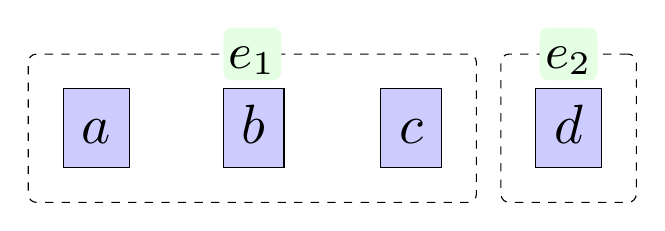
\begin{tikzpicture}[
			scale=2,
			transform shape,
			every node/.style={
					draw,
					fill=blue!20,
					text height=1.5ex, % Height above the baseline
					text depth=0.25ex  % Depth below the baseline
				}
		]
		\node (n0) at (0, 0) {$a$};
		\node (n1) at (1, 0) {$b$};
		\node (n2) at (2, 0) {$c$};
		\node (n3) at (3, 0) {$d$};

		\node[
			draw=none,
			fill=none,
			inner sep=12pt,         % Space between nodes and the box border
			fit=(n0) (n1) (n2),     % Tells TikZ which nodes to enclose
		] (box) {};

		\draw[dashed, rounded corners=3pt]
		(box.north east) --
		(box.north west) node[midway, draw=none, fill=green!10, inner sep=1pt] {\small $e_1$} --
		(box.south west) --
		(box.south east) -- cycle;

		\node[
			draw=none,
			fill=none,
			inner sep=12pt,         % Space between nodes and the box border
			fit=(n3),     % Tells TikZ which nodes to enclose
		] (box2) {};

		\draw[dashed, rounded corners=3pt]
		(box2.north east) --
		(box2.north west) node[midway, draw=none, fill=green!10, inner sep=1pt] {\small $e_2$} --
		(box2.south west) --
		(box2.south east) -- cycle;
	\end{tikzpicture}
\end{figure}

If we abstract from the contents of the E-nodes, we can just think of each E-node as a unique \emph{constant}. Then the problem is to determine if an equation between constants $a = b$ follows from a set of equations $\Gamma = \{c = d, \ldots e = f\}$. For this problem, we have a beautiful solution that comes with an efficient implementation. This is what we would love to see for every fragment, but things become more difficult as we introduce more complexity.

We recall some standard notions. Given a set, an \textbf{equivalence relation} over that set is a reflexive, symmetric, and transitive relation. Given an equivalence relation, we can take the \textbf{quotient} of the set by it, a set containing a single element for each \textbf{equivalence class} of elements in the original set.

The \emph{Union-Find} data structure is an efficient means to represent an equivalence relation over a set, and to update it either by extending the underlying set or by merging two equivalence classes. Union-find avoids any fiddly manipulation with reflexivity, symmetry, and transitivity, and focuses on a \emph{semantic} characterization of equivalence relations: a function $r : A \rightarrow B$ splits the domain $A$ into equivalence classes based on the equality of their images in $B$: define $R$ by $R = \{(a, b) \mid r(a) = r(b)\}$. In this, $B$ \emph{is} just the set of equivalence classes, and $r$ \emph{is} just the quotient.

% an equivalence relation on a set partitions it into disjoint sets of equivalence classes. And an equivalence relation on terms is exactly a model of equality: it is closed under reflexivity, symmetry, and transitivity, so it is an \textbf{equivalence relation} The theory of equality between constants is usually presented with three axiom schemas: reflexivity, $\vdash a = a$, symmetry, $a = b \vdash b = a$, and transitivity, $a = b, b = c \vdash a = c$. However, the standard solution of this problem abandons any fiddly manipulation with these identities and focuses on an entirely \emph{semantic} characterization of equality: an equivalence relation on a set partitions it into disjoint sets of \textbf{equivalence classes}. And an equivalence relation on terms is exactly a model of equality: it is closed under reflexivity, symmetry, and transitivity, so it is an \textbf{equivalence relation} Let's phrase this more symbolically. Take a set of constants $A$, an equivalence relation $R \subseteq A \times A$ is a relation such that for every $a \in A$, $(a, a) \in R$, amd for every $a, b \in A$, $(a, b) \in R$ implies $(b, a) \in R$, and for every $a, b, c \in A$, $(a, b) \in R$ and $(b, c) \in R$ implies $(a, c) \in R$. Then an equivalence class of a particular element $a \in A$ is the set $\{b \mid (a, b) \in R\}$. We denote the set of equivalence classes by $A / R$, and there is a function $r : A \rightarrow A/R$ given by $r(a) = \{b \mid (a, b) \in R\}$. If $r(a) = r(b)$, then $(a, b) \in R$.

Using this fact, we can sketch an implementation that maintains this mapping $r$ from a set of constants to a set of equivalence classes. To start off with, we don't need to represent the codomain $B$ in any fancy way: we just assign a new identifier to each equivalence class. Then, a basic implementation is just an array or table with indexes in $A$ and entries in some set of identifiers for equivalence classes.

This representation potentially requires a bit of work to update: if we want to take into account a new equation $a = b$ with an existing $r$, we need to set all things mapping to $r(a)$ and $r(b)$ to the same identifier. It is possible to lazily update the union-find whenever doing a find, effectively storing a function $q$ whose fixed-point is $r$, which makes the running time for $n$ union and find operations be just $O(n \alpha(n))$, where $\alpha$ is the inverse Ackermann function, a very slow-growing function \fxerror{source}.

\section{Congruence relations and Congruence-closure} \label{egraphs2}
A congruence relation on a set of terms is one that respects the function symbols: for instance, if $f$ is a function symbol of arity 3, and $s_1 = t_1$, $s_2 = t_2$, and $s_3 = t_3$, then $f(s_1, s_2, s_3) = f(t_1, t_2, t_3)$. In general, we get the following axiom schema: for each $n$-ary symbol $f$, $a_1 = b_1, \ldots, a_n = b_n \vdash f(a_1, \ldots, a_n) = f(b_1, \ldots, b_n)$. This is the larger fragment solved by a congruence-closure data structure.

We keep a union-find storing equivalence classes of \textbf{E-nodes}\footnote{`E' in E-graph, E-node, E-class, etc., stands for equality}: as we have seen, if $s = t$, then we don't need to waste space represent both $f(s)$ and $f(t)$, given that these are identical. So, we restrict ourselves to keeping not a set of terms, but a set of `lifted' terms like $f(e_1)$, if $e_1$ is the name we assign to the class containing $s$ and $t$.

This has the potential to save an infinite amount of space: if we have the input equation $f(a) = a$, then the equivalence class of $a$ up to congruence includes the infinite set of terms $a, f(a), f(f(a)), \ldots$. So the `lifting' of terms to act on equivalence classes lets us represent every congruence relation in a finite way.

Indeed, this idea yields the congruence-closure algorithm for deciding equality over any set of equations. We will simply refer to the congruence-closure structure as an \textbf{E-graph}, although the term E-graph is commonly used when we also include equality saturation (\ref{eqsat}).

We will show the congruence-closure algorithm running on our previous set of equations

\begin{align*}
f(a) &= a, \\
g(f(f(a)), b) &= g(a, g(a, b)) \\
g(f(a), b) &= b
\end{align*}

We can build the E-graph over these equations as follows:

First, we add all terms with no subterms, namely $a$ and $b$. These each get a distinct equivalence class.

\begin{figure}[h!]
	\centering
	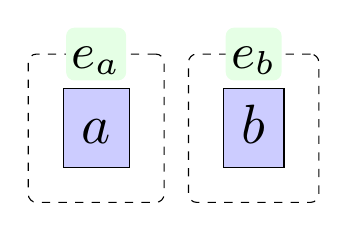
\begin{tikzpicture}[
			scale=2,
			transform shape,
			every node/.style={
					draw,
					fill=blue!20,
					text height=1.5ex, % Height above the baseline
					text depth=0.25ex  % Depth below the baseline
				}
		]
		\node (n0) at (0, 0) {$a$};
		\node (n1) at (1, 0) {$b$};

		\node[
			draw=none,
			fill=none,
			inner sep=12pt,         % Space between nodes and the box border
			fit=(n0),     % Tells TikZ which nodes to enclose
		] (box) {};

		\draw[dashed, rounded corners=3pt]
		(box.north east) --
		(box.north west) node[midway, draw=none, fill=green!10, inner sep=1pt] {\small $e_a$} --
		(box.south west) --
		(box.south east) -- cycle;

		\node[
			draw=none,
			fill=none,
			inner sep=12pt,         % Space between nodes and the box border
			fit=(n1),     % Tells TikZ which nodes to enclose
		] (box2) {};

		\draw[dashed, rounded corners=3pt]
		(box2.north east) --
		(box2.north west) node[midway, draw=none, fill=green!10, inner sep=1pt] {\small $e_b$} --
		(box2.south west) --
		(box2.south east) -- cycle;
	\end{tikzpicture}
\end{figure}

Next we add $f(a)$: $a$ is represented by $e_a$, so we represent $f(a)$ by $f(e_a)$, and can graphically depict this with an arrow:

\begin{figure}[h!]
	\centering
	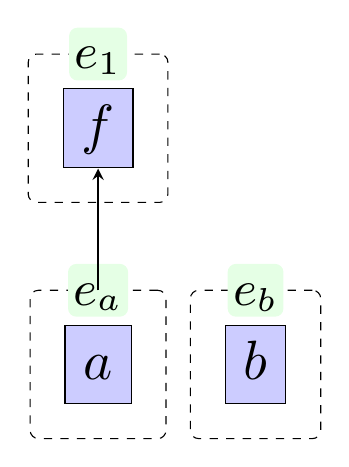
\begin{tikzpicture}[
			scale=2,
			transform shape,
			every node/.style={
					draw,
					fill=blue!20,
					text height=1.5ex, % Height above the baseline
					text depth=0.25ex  % Depth below the baseline
				}
		]
		\node (n0) at (0, 0) {$a$};
		\node (n1) at (1, 0) {$b$};
		\node (n2) at (0, 1.5) {$f$};

		\node[
			draw=none,
			fill=none,
			inner sep=12pt,         % Space between nodes and the box border
			fit=(n0),     % Tells TikZ which nodes to enclose
		] (box) {};

		\draw[dashed, rounded corners=3pt]
		(box.north east) --
		(box.north west) node[midway, draw=none, fill=green!10, inner sep=1pt] {\small $e_a$} --
		(box.south west) --
		(box.south east) -- cycle;

		\node[
			draw=none,
			fill=none,
			inner sep=12pt,         % Space between nodes and the box border
			fit=(n1),     % Tells TikZ which nodes to enclose
		] (box2) {};

		\draw[dashed, rounded corners=3pt]
		(box2.north east) --
		(box2.north west) node[midway, draw=none, fill=green!10, inner sep=1pt] {\small $e_b$} --
		(box2.south west) --
		(box2.south east) -- cycle;
		
		\node[
			draw=none,
			fill=none,
			inner sep=12pt,         % Space between nodes and the box border
			fit=(n2),     % Tells TikZ which nodes to enclose
		] (box3) {};

		\draw[dashed, rounded corners=3pt]
		(box3.north east) --
		(box3.north west) node[midway, draw=none, fill=green!10, inner sep=1pt] {\small $e_1$} --
		(box3.south west) --
		(box3.south east) -- cycle;
		
		\draw[->, >=stealth, thick] (box.north) -- (n2.south);
	\end{tikzpicture}
\end{figure}

Now we have represented both terms in the equation $f(a) = a$, so we merge the resulting equivalence classes:

\begin{figure}[h!]
	\centering
	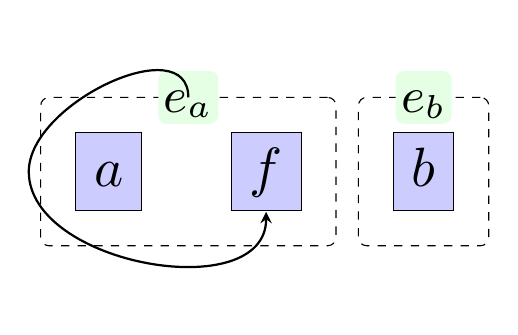
\begin{tikzpicture}[
			scale=2,
			transform shape,
			every node/.style={
					draw,
					fill=blue!20,
					text height=1.5ex, % Height above the baseline
					text depth=0.25ex  % Depth below the baseline
				}
		]
		\node (n0) at (0, 0) {$a$};
		\node (n1) at (2, 0) {$b$};
		\node (n2) at (1, 0) {$f$};

		\node[
			draw=none,
			fill=none,
			inner sep=12pt,         % Space between nodes and the box border
			fit=(n0) (n2),     % Tells TikZ which nodes to enclose
		] (box) {};

		\draw[dashed, rounded corners=3pt]
		(box.north east) --
		(box.north west) node[midway, draw=none, fill=green!10, inner sep=1pt] {\small $e_a$} --
		(box.south west) --
		(box.south east) -- cycle;

		\node[
			draw=none,
			fill=none,
			inner sep=12pt,         % Space between nodes and the box border
			fit=(n1),     % Tells TikZ which nodes to enclose
		] (box2) {};

		\draw[dashed, rounded corners=3pt]
		(box2.north east) --
		(box2.north west) node[midway, draw=none, fill=green!10, inner sep=1pt] {\small $e_b$} --
		(box2.south west) --
		(box2.south east) -- cycle;
		
		\draw[->, >=stealth, thick] (box.north) to[out=90, in=90, looseness=1] ([xshift=-0.5ex]box.west) to[out=270, in=270, looseness=1] (n2.south);
	\end{tikzpicture}
\end{figure}

This merged class represents all of $a, f(a), f(f(a)), \ldots$.

Now we look at representing some of the input terms using the function symbol $g$. Using our existing equivalence classes, $f(f(a))$ is represented by $f(f(e_a)$ is represented by $f(e_a)$ is represented by $e_a$, so $g(f(f(a)), b)$ is represented by $g(e_a, e_b)$, which is not yet in our E-graph. $g(e_a, e_b)$ represents all of $g(f(f(a)), b)$, $g(a, b)$, and $g(f(a), b)$.

\begin{figure}[h!]
	\centering
	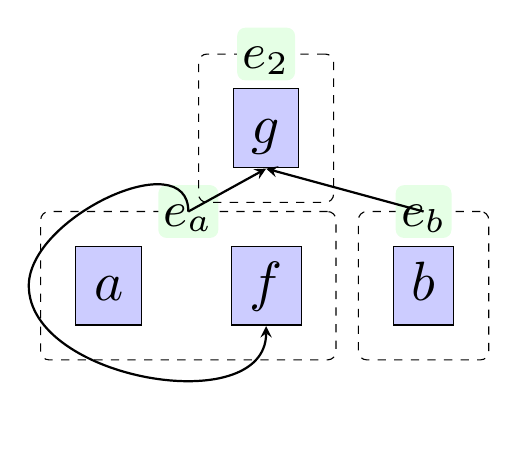
\begin{tikzpicture}[
			scale=2,
			transform shape,
			every node/.style={
					draw,
					fill=blue!20,
					text height=1.5ex, % Height above the baseline
					text depth=0.25ex  % Depth below the baseline
				}
		]
		\node (n0) at (0, 0) {$a$};
		\node (n1) at (2, 0) {$b$};
		\node (n2) at (1, 0) {$f$};
		\node (n3) at (1, 1) {$g$};

		\node[
			draw=none,
			fill=none,
			inner sep=12pt,         % Space between nodes and the box border
			fit=(n0) (n2),     % Tells TikZ which nodes to enclose
		] (box) {};

		\draw[dashed, rounded corners=3pt]
		(box.north east) --
		(box.north west) node[midway, draw=none, fill=green!10, inner sep=1pt] {\small $e_a$} --
		(box.south west) --
		(box.south east) -- cycle;

		\node[
			draw=none,
			fill=none,
			inner sep=12pt,         % Space between nodes and the box border
			fit=(n1),     % Tells TikZ which nodes to enclose
		] (box2) {};

		\draw[dashed, rounded corners=3pt]
		(box2.north east) --
		(box2.north west) node[midway, draw=none, fill=green!10, inner sep=1pt] {\small $e_b$} --
		(box2.south west) --
		(box2.south east) -- cycle;
		
		\node[
			draw=none,
			fill=none,
			inner sep=12pt,         % Space between nodes and the box border
			fit=(n3),     % Tells TikZ which nodes to enclose
		] (box3) {};

		\draw[dashed, rounded corners=3pt]
		(box3.north east) --
		(box3.north west) node[midway, draw=none, fill=green!10, inner sep=1pt] {\small $e_2$} --
		(box3.south west) --
		(box3.south east) -- cycle;
		
		\draw[->, >=stealth, thick] (box.north) to[out=90, in=90, looseness=1] ([xshift=-0.5ex]box.west) to[out=270, in=270, looseness=1] (n2.south);
		
		\draw[->, >=stealth, thick] (box.north) -- (n3.south);
		\draw[->, >=stealth, thick] (box2.north) -- (n3.south);
	\end{tikzpicture}
\end{figure}

The last term to represent is then $g(a, g(a, b))$, which is represented by $g(e_a, e_2)$.

\begin{figure}[h!]
	\centering
	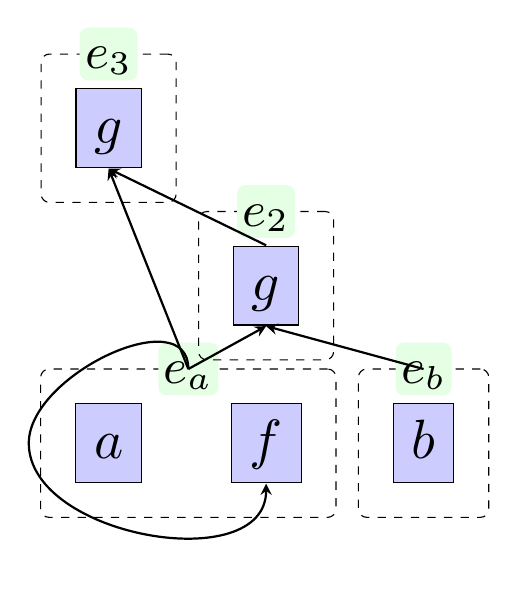
\begin{tikzpicture}[
			scale=2,
			transform shape,
			every node/.style={
					draw,
					fill=blue!20,
					text height=1.5ex, % Height above the baseline
					text depth=0.25ex  % Depth below the baseline
				}
		]
		\node (n0) at (0, 0) {$a$};
		\node (n1) at (2, 0) {$b$};
		\node (n2) at (1, 0) {$f$};
		\node (n3) at (1, 1) {$g$};
 		\node (n4) at (0, 2) {$g$};

		\node[
			draw=none,
			fill=none,
			inner sep=12pt,         % Space between nodes and the box border
			fit=(n0) (n2),     % Tells TikZ which nodes to enclose
		] (box) {};

		\draw[dashed, rounded corners=3pt]
		(box.north east) --
		(box.north west) node[midway, draw=none, fill=green!10, inner sep=1pt] {\small $e_a$} --
		(box.south west) --
		(box.south east) -- cycle;

		\node[
			draw=none,
			fill=none,
			inner sep=12pt,         % Space between nodes and the box border
			fit=(n1),     % Tells TikZ which nodes to enclose
		] (box2) {};

		\draw[dashed, rounded corners=3pt]
		(box2.north east) --
		(box2.north west) node[midway, draw=none, fill=green!10, inner sep=1pt] {\small $e_b$} --
		(box2.south west) --
		(box2.south east) -- cycle;
		
		\node[
			draw=none,
			fill=none,
			inner sep=12pt,         % Space between nodes and the box border
			fit=(n3),     % Tells TikZ which nodes to enclose
		] (box3) {};

		\draw[dashed, rounded corners=3pt]
		(box3.north east) --
		(box3.north west) node[midway, draw=none, fill=green!10, inner sep=1pt] {\small $e_2$} --
		(box3.south west) --
		(box3.south east) -- cycle;
		
		\node[
			draw=none,
			fill=none,
			inner sep=12pt,         % Space between nodes and the box border
			fit=(n4),     % Tells TikZ which nodes to enclose
		] (box4) {};

		\draw[dashed, rounded corners=3pt]
		(box4.north east) --
		(box4.north west) node[midway, draw=none, fill=green!10, inner sep=1pt] {\small $e_3$} --
		(box4.south west) --
		(box4.south east) -- cycle;
		
		\draw[->, >=stealth, thick] (box.north) to[out=90, in=90, looseness=1] ([xshift=-0.5ex]box.west) to[out=270, in=270, looseness=1] (n2.south);
		
		\draw[->, >=stealth, thick] (box.north) -- (n3.south);
		\draw[->, >=stealth, thick] (box2.north) -- (n3.south);
		\draw[->, >=stealth, thick] (box.north) -- (n4.south);
		\draw[->, >=stealth, thick] (n3.north) -- (n4.south);
	\end{tikzpicture}
\end{figure}

Now, we need to process the remaining two equations. $g(f(f(a)), b) = g(a, g(a, b))$ tells us to merge the equivalence classes $e_2$ and $e_3$. $g(f(a), b) = b$ tells us to merge $e_2$ and $e_b$.

\begin{figure}[h!]
	\centering
	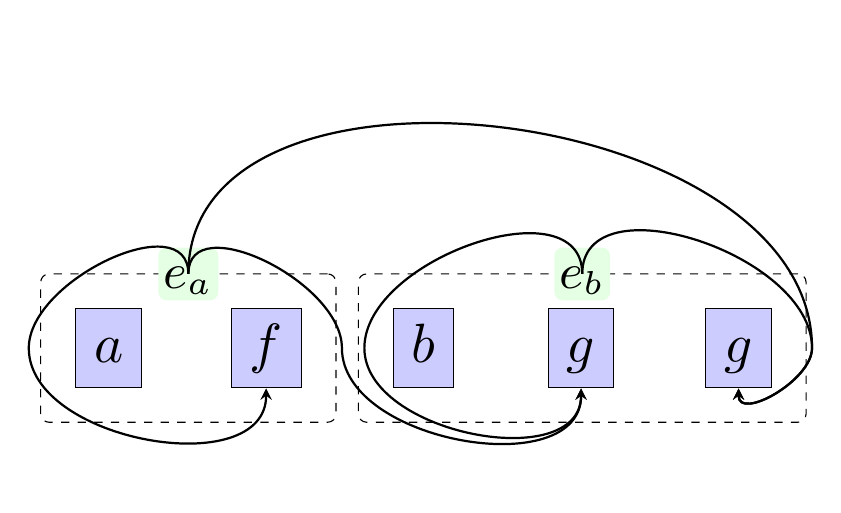
\begin{tikzpicture}[
			scale=2,
			transform shape,
			every node/.style={
					draw,
					fill=blue!20,
					text height=1.5ex, % Height above the baseline
					text depth=0.25ex  % Depth below the baseline
				}
		]
		\node (n0) at (0, 0) {$a$};
		\node (n2) at (1, 0) {$f$};
		\node (n1) at (2, 0) {$b$};
		\node (n3) at (3, 0) {$g$};
 		\node (n4) at (4, 0) {$g$};

		\node[
			draw=none,
			fill=none,
			inner sep=12pt,         % Space between nodes and the box border
			fit=(n0) (n2),     % Tells TikZ which nodes to enclose
		] (box) {};

		\draw[dashed, rounded corners=3pt]
		(box.north east) --
		(box.north west) node[midway, draw=none, fill=green!10, inner sep=1pt] {\small $e_a$} --
		(box.south west) --
		(box.south east) -- cycle;

		\node[
			draw=none,
			fill=none,
			inner sep=12pt,         % Space between nodes and the box border
			fit=(n1) (n3) (n4),     % Tells TikZ which nodes to enclose
		] (box2) {};

		\draw[dashed, rounded corners=3pt]
		(box2.north east) --
		(box2.north west) node[midway, draw=none, fill=green!10, inner sep=1pt] {\small $e_b$} --
		(box2.south west) --
		(box2.south east) -- cycle;
		
		\draw[->, >=stealth, thick] (box.north) to[out=90, in=90, looseness=1] ([xshift=-0.5ex]box.west) to[out=270, in=270, looseness=1] (n2.south);
		
		\draw[->, >=stealth, thick] (box.north) to[out=90, in=90, looseness=1] ([xshift=0.25ex]box.east) to[out=270, in=270, looseness=1] (n3.south);
		
		\draw[->, >=stealth, thick] (box2.north) to[out=90, in=90, looseness=1] ([xshift=0.25ex]box2.west) to[out=270, in=270, looseness=1] (n3.south);
		
		\draw[->, >=stealth, thick] (box.north) to[out=90, in=90, looseness=1] ([xshift=0.25ex]box2.east) to[out=270, in=270, looseness=1] (n4.south);
		
		\draw[->, >=stealth, thick] (box2.north) to[out=90, in=90, looseness=1] ([xshift=0.25ex]box2.east) to[out=270, in=270, looseness=1] (n4.south);
		
	\end{tikzpicture}
\end{figure}

The last step is to apply to rule of \emph{congruence}. Our graph now has two nodes representing $g(e_a, e_b)$. We merge them; as they are already in the same class, there is no further work to be done:

\begin{figure}[h!]
	\centering
	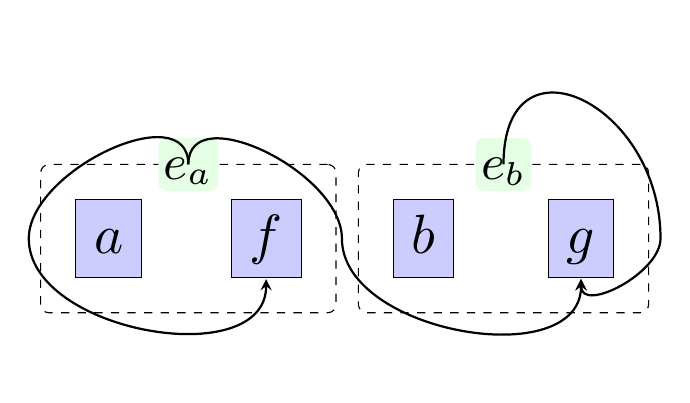
\begin{tikzpicture}[
			scale=2,
			transform shape,
			every node/.style={
					draw,
					fill=blue!20,
					text height=1.5ex, % Height above the baseline
					text depth=0.25ex  % Depth below the baseline
				}
		]
		\node (n0) at (0, 0) {$a$};
		\node (n2) at (1, 0) {$f$};
		\node (n1) at (2, 0) {$b$};
		\node (n3) at (3, 0) {$g$};

		\node[
			draw=none,
			fill=none,
			inner sep=12pt,         % Space between nodes and the box border
			fit=(n0) (n2),     % Tells TikZ which nodes to enclose
		] (box) {};

		\draw[dashed, rounded corners=3pt]
		(box.north east) --
		(box.north west) node[midway, draw=none, fill=green!10, inner sep=1pt] {\small $e_a$} --
		(box.south west) --
		(box.south east) -- cycle;

		\node[
			draw=none,
			fill=none,
			inner sep=12pt,         % Space between nodes and the box border
			fit=(n1) (n3),     % Tells TikZ which nodes to enclose
		] (box2) {};

		\draw[dashed, rounded corners=3pt]
		(box2.north east) --
		(box2.north west) node[midway, draw=none, fill=green!10, inner sep=1pt] {\small $e_b$} --
		(box2.south west) --
		(box2.south east) -- cycle;
		
		\draw[->, >=stealth, thick] (box.north) to[out=90, in=90, looseness=1] ([xshift=-0.5ex]box.west) to[out=270, in=270, looseness=1] (n2.south);
		
		\draw[->, >=stealth, thick] (box.north) to[out=90, in=90, looseness=1] ([xshift=0.25ex]box.east) to[out=270, in=270, looseness=1] (n3.south);
		
		\draw[->, >=stealth, thick] (box2.north) to[out=90, in=90, looseness=2]		([xshift=0.5ex]box2.east) to[out=270, in=270, looseness=1] (n3.south);
		
	\end{tikzpicture}
\end{figure}

However, in some cases applying congruence can cause a chain of merges. This process terminates as there is a maximal state of finite size (an E-graph assigning all nodes to the same equivalence class), so any potential infinite chain of congruence steps will reach a fixed point after finitely many steps.

Note the final E-graph has two \emph{cycles}: $f(e_a) = e_a$ and $g(e_a, e_b) = e_b$. In general, we might have cycles going through multiple intermediary nodes: $f(\ldots g(\ldots e_1 \ldots) \ldots) = e_1$. Cycles become very important in the analysis of how theories fare with E-graphs under equality saturation (section \ref{howfare}).

For congruence closure, and thus E-graphs, the laziness possible in the union-find seems difficult to make use of, as we need to detect the congruence $f(a_1, \ldots, b, \ldots, a_n) = f(a_1, \ldots, b, \ldots, a_n)$ once $b$ and $c$ have been equated; it is not enough to just `discover' that $b = c$ when calling find on $b$ or $c$ or one of their equivalents, as such a find call is not guaranteed to happen at any particular point before we need to discover the congruence.

%\subsection{A more formal description}
%We will maintain a union-find structure representing a quotient function $r : E \rightarrow E/R$; $E$ is some superset of the constants $A$ that includes an element for every E-node. We will call these \textbf{E-nodes}, and elements of the set $E/R$ \textbf{E-classes}. We introduce, for each $n$-ary function symbol $f$, a mapping $f_r : (E/R)^n \rightarrow E/R$. Unfortunately, we now have two objects to keep in sync if we hope to represent $r$ via the efficient union-find structure from before. In particular, if $r$ is altered to merge two equivalence classes, we then have  to scan through our representation of $f_r$ to see if we encounter a case where two equal tuples are mapped to unequal representatives. In that case, we must merge the representatives according to congruence, and then go back and check if this new merge has any consequences, and so forth.

%This system, where we bounce new equalities between data structures, is rather typical of \textbf{theory combination} \fxerror{add ref to later part}. 

%The resulting combined data structure is known as a \textbf{congruence-closure} data structure \fxerror{source}. We nonetheless will not refer to it as \emph{the} congruence-closure data structure, given that it is far less canonical than the union-find structure. In particular, exactly how newly-congruent items are discovered in each $f_r$ provides an axis of variation. \fxerror{this is a bit mean-spirited. I guess I was a bit annoyed at how formalizing Downey-Sethi-Tarjan is a bit of a slog :)}

\subsection{Congruence closure builds a rewrite system}
We can read off a set of equations from our final E-graph:

\begin{align*}
	a &= e_a \\
	f(e_a) &= e_a \\
	b &= e_b \\
	g(e_a, e_b) &= e_b \\
\end{align*}

Given this resulting set of equations, we can determine if any two terms at all are equal under our initial set of equations: simply reduce the terms by treating these equations as a \emph{rewrite system}, read from left-to-right, and see if the normal forms are the same. \fxerror{Refs for connections to rewrite systems}.

\section{Equality saturation} \label{eqsat}
Now that we can reason about the logical consequences of (ground) equations, we look to solve the problem of reasoning with identities. The method of \textbf{equality saturation} is what we will focus on in this thesis.

The key idea is that, given a representation of a congruence relation, we \emph{E-match} each  identity $\forall a_1, \ldots, a_n. s_1 = s_2$ against the congruence relation to find all instances $s_1[t_1/a_1, \ldots, t_n/a_n]$ and $s_2[t_1/a_1, \ldots, t_n/a_n]$. Then, we find the representatives of these two terms. If they are not equal, we have found two equivalence classes to merge to take into account the identity. We will refer to this as a \textbf{proper merge}.

Unfortunately, proper merges are not sufficient. If we consider the associative identity $\forall a b c.\; a + (b + c) = (a + b) + c$, and we begin with the two equalities $u = w + (x + (y + z))$ and $v = ((w + x) + y) + z$, we would like to prove the theorem that

\begin{align*}
	(\forall a b c.\; a + (b + c) = (a + b) + c), \\
	u = w + (x + (y + z)),                        \\
	v = ((w + x) + y) + z                         \\
	\vdash u = v
\end{align*}

However, the attempt to prove even the first step, that $w + (x + (y + z)) = (w + x) + (y + z)$, founders. Our representation includes no equivalence class to represent $(w + x) + (y + z)$, and so there are no equivalence classes to merge.

The `solution' is to introduce the possibility of \textbf{inserting} new classes during the procedure. For instance, we can find an instance $s_1 = s_2$ of an identity such that $s_1$ maps to a known equivalence class but $s_2$ doesn't. We seed $s_2$ as a new term by calculating its equivalence class, potentially introducing a new class if no prior one exists, and then merging the equivalence classes of $s_1$ and $s_2$. We call this mix of seeing and a proper merge an \textbf{improper merge}.

Insertion has one key problem: we now have no guarantees the process of merging will terminate. With only proper merges, there are a finite set of input terms and thus a finite bound on the equivalence relation we maintain. Thus, eventually we will get to a point where no merge changes the equivalence relation, and we have reached \textbf{saturation}. Introducing new classes for inserted terms now means that saturation is no longer guaranteed to be reached at any point, and worse, the strategy for insertion and merging now can affect whether or not saturation is reached.

To even get a \emph{semi-decision procedure}, where we aim to prove a specific equality if it exists and can fail otherwise, we must ensure that the insertion and merging processes are sufficiently \emph{fair} (in the sense of `fair' as used in concurrent programming): we must have some strategy to ensure every possible term that could be inserted \emph{does} get inserted eventually, or we might get stuck inserting other terms infinitely while nonetheless not making progress on the goal.

In some sense, this is to be expected, as even for just equational theorem proving, there are theories which are known to be undecidable. However, even when the process of E-matching, inserting and merging doesn't terminate, we can consider the infinite fixed-point of this process as the `semantics' of our E-graph \citep{suciu_semantic_2025}, and this will be what we will preserve in the shift to EMTs. This process will be referred to as the `equality saturation outer loop'. A schematic form is as follows:

\begin{enumerate}
	\item Insert all the starting terms into the E-graph
	\item Repeat until fixed point:
	      \begin{enumerate}
		      \item \textbf{E-match} an identity against the E-graph, finding all ground instances of one side of the identity that exist in the E-graph.
		      \item \textbf{Insert} Using the substitution from the previous step, construct the term resulting from applying the substitution to the other side of the identity. If it is not already represented by the E-graph, add it to the E-graph.
		      \item \textbf{Merge} the E-classes representing both sides of the equality above.
		      \item \textbf{Rebuild} the graph, using the rules of congruence closure
	      \end{enumerate}
\end{enumerate}

If the fixed point is reached, we call the graph \textbf{saturated}.

\subsection{A few variations}
We can do several matches/insertions/merges in between rebuilding; it is sufficient that rebuilding is \emph{eventually} run after changes to the E-graph \citep{willsey_egg_2021}.

There are plenty of extensions to the outer loop that include things such as conditional reasoning (along the lines of: if $a = b$, then assert that $c = d$ by merging classes) or E-class analyses (\citep{willsey_egg_2021}).

%\section{E-graphs as tree automata} \label{treeauto}
%\fxerror{Things about rational sets, tree automata mod theories? and recognizable vs rational?}

%\citep{koppel_version_2021} \citep{wang_e-graphs_nodate}

%\emph{A much better source: \citep{suciu_semantic_2025}. Actually, I should use this source more often...}

% \section{Terms, signatures, and theories formalized} \label{termsig}
% \fxerror{Where should this go?}

% A \textbf{signature} is a set $\Sigma$ of function symbols with an arity given by a function $\alpha : \Sigma \rightarrow \mathbb{N}$. Given a set of constants $A$, a \textbf{term fragment} $\Sigma(A)$ is a pair of an element of $f \in \Sigma$ together with a list of elements of $A$ of length $\alpha(f)$. A \textbf{term} over $A$, denoted by $\Sigma^*(A)$, is defined inductively as either a constant $a \in A$ or a term fragment over $\Sigma^*(A)$.

% Given a term in $\Sigma^*(A)$, we can extend it to be over more constants $\Sigma^*(A + B)$ in the obvious way, denoting by $+$ the disjoint union of sets. We will often use auxiliary constants written as $a, b, c$ etc., but these should be distinguished from the notion of a variable in an identity defined below.

% An interpretation of a signature $\Sigma$ is a \textit{carrier} set $A$ together with a function $a : \Sigma(A) \rightarrow A$ that interprets term fragments, from which the interpretation of terms in $\Sigma^*(A)$ is given by recursive application of $a$, interpreting from the leaves to the root in the natural way. We will denote this by $\textbf{fold}(a) : \Sigma^*(A) \rightarrow A$.

% Given a signature, there is a standard notion of first-order logic\footnote{given the fragment we will consider in this thesis, there is no actual distinction between classical and intuitionistic first-order logic. [source about Horn(CL) = Horn(I)]} over the terms of $\Sigma^*(A)$. More specifically, we will consider \textbf{theories}, which are conjunctions of identities, where an \textbf{identity} is a proposition of the form $\forall x_1. \dotsi \forall x_i. t_1 = t_2$ where $t_1$ and $t_2$ are terms over $A + \{x_1, \dotsc x_i\}$. Note that the number of quantifiers can also be 0.
% A \textbf{ground instance} of an identity is an equation of the form $\sigma(t_1) = \sigma(t_2)$, where $\sigma$ is a \textbf{substitution} that maps variables in $\{x_1, \dotsc x_i\}$ to terms over $A$. We will generally use \textbf{equation} to mean any equation between terms in the \textbf{ground fragment} $\Sigma^*(A)$, while reserving identity for universally quantified equations.\\

% \begin{ex}
% 	Let $\Sigma = \{f, g\}$ and $\alpha(f) = 2, \alpha(g) = 1$. If $A = \{x, y, z\}$, then $f(x, y)$, $g(z)$, and $f(y, y)$ are elements of $\Sigma(A)$. In addition, $x$, $f(f(x, y), g(x))$, and $g(g(g(z)$ are elements of $\Sigma^*(A)$.

% 	If we have the theory $T = (\forall a b. f(a, b) = g(f(a, b))) \wedge (\forall a. g(a) = g(g(a)))$, then we can derive the ground equation $f(x, g(y)) = g(f(x, g(y))$ from $T$ by a substitution in the first identity of $\sigma(a) = x, \sigma(b) = g(y)$.
% \end{ex}

% \section{Matching, merging, seeding, and canonicalization formalized}
% \fxerror{To be moved}
% Here we spell out the relevant procedures in some detail, given as they will be central to our generalization to EMTs \ref{coreres}.

% A congruence closure structure $(A, E, b : A \rightarrow E, q : E \rightarrow E, c : (f : \Sigma) \rightharpoonup E^{\alpha(f)} \rightarrow E)$ consists of a set of constants $A$, a set of `E-node names' $E$, a name for each constant $b : A \rightarrow E$, a union-find map $q$, and a partial function-symbol map $c$, where $c_f : E^{\alpha(f)} \rightarrow E$ is the function map for a particular symbol $f \in \Sigma$. Particular entries $c_f(e_1 \in E, \ldots, e_n \in E) \mapsto e \in E$ are called \textbf{E-nodes}. Fixed points of the map $q$ are called \textbf{E-classes}.

% We will use the term E-graph both for this abstract structure as well as concrete implementations, for which some auxiliary maps are useful to speed up certain operations.

% The relation $=_q$ is defined as $\{(a, b) \mid q^*(a) = q^*(b)\}$ where $q^*$ is the fixed point of q.

% A term fragment $f(e_1, \ldots, e_n) : \Sigma(E)$ is represented by the E-class $e$ in an E-graph if $c_f(e_1, \ldots, e_n)$ maps to some $f$ where $f =_q e$. A term $t \in \Sigma^*(A + E)$ is represented by $e$ if it is simply a node name $f \in E$ such that $f =_q e$, or if it is a constant $a \in A$ and $b(a) =_q e$, or if it is a term fragment $f(t_1, \ldots, t_n)$ such that $t_i$ are represented by $e_i$ and $f(e_1, \ldots, e_n)2$ is represented by $e$.

% The matching problem is the following: for a pattern $p \in \Sigma^*(A + S)$, is there a substitution $\sigma : S \rightarrow \Sigma^*(A + E)$ such that the term $p \sigma \in \Sigma^*(A + E)$ is represented by the E-graph?

% Merging is the process of taking two elements $e_1, e_2 \in E$ and updating $q$ so that $e_1 =_q e_2$ .

% Seeding takes a term $t$ and updates the E-graph so that there is some $e \in E$ such that $e$ represents $t$.

% Canonicalization updates $q$ and the function-symbol maps $c_f$ to ensure that if $e_1 =_q e_2,  \ldots, e_{n1} =_q e_{n2}$, then $c_f(e_1, \ldots, e_{n1}) =_q c_f(e_2, \ldots, e_{n2})$. In general, this is done by a fixed-point method of finding pairs of tuples such that the corresponding elements are equivalent under $=_q$ while $c_f$ maps them to inequivalent elements, and then merging.

\subsection{How E-graphs handle ordinary critical pairs, but not AC-critical pairs}

To get a better perspective on this problem, we use ideas from rewriting and in particular the notion of Abstract Congruence Closure (\citep{bachmair_abstract_2000}). We can think of E-graphs as presenting a rewriting system, and the above E-graph as containing the rewrite rules

\begin{align*}
  b &\rightarrow e_b \\
  c &\rightarrow e_c \\
  d &\rightarrow e_d \\
	a + e_b &\rightarrow e_b \\
	a + a &\rightarrow e_c \\
	e_c + e_b &\rightarrow e_d
\end{align*}

(A distinguished equivalence class for $a$ is omitted to make the diagram easier to follow)

A critical pair for a rewriting system is a term that can be rewritten two different ways\footnote{It is also required to be minimal among such terms, but we gloss over this here}.
The perspective of Abstract Congruence Closure is that congruence closure, the core algorithm for `rebuilding' E-graphs, constructs a \emph{confluent term rewriting system} on an extended signature. Handling critical pairs is required for confluence, which ensures that a term rewrites into a single result; if we have a term $t$ that rewrites to both $e_a$ and $e_b$, we ought to automatically \emph{deduce} that the E-classes $e_a$ and $e_b$ should be merged.

By introducing new constants $e_1, e_2, \ldots$ as E-ids, we can `flatten' an input term $f(\ldots, g(h(\ldots)), \ldots)$ into just $f(\ldots, e_i, \ldots)$ and then assign it the name $e_k$ for some $k$. 

Now, to ensure the convergence of the rewrite system, we can look at two kinds of cases where a term could rewrite in two ways:

$e_1 \leftarrow f(\ldots e_i \ldots) \rightarrow e_2$ in which case, we ought to deduce that $e_1 = e_2$. This corresponds to merging E-classes which would contain duplicates of the same E-node.

$f(\ldots e_i \ldots) \rightarrow e_1$ and $e_i \rightarrow e_2$, in which case we ought to deduce that \\ $f(\ldots e_2 \ldots) = e_1$. This corresponds to canonizing the E-nodes using the union-find structure.

By fixpoint propagation, resolving these two cases are enough to resolve all cases of critical pairs with overlaps on more deeply nested subterms.

E-graph rebuilding can handle ordinary critical pairs, but this doesn't cover our above example, which is an \emph{AC-critical pair}. 

\subsection{Equality satuation: \\ handling AC-critical pairs by brute force}
E-graphs (not modulo theories) handle AC-critical pairs the same way as critical pairs for any other theory, with equality saturation: we \emph{ground} the AC identities by matching either side with the E-graph, and adding the equivalent other side (if it is not present) and merging the equivalence classes corresponding to either side.

Why do E-graphs fare poorly with AC? The two identities, (A) $\forall xyz.\; x + (y + z) = (x + y) + z$ and (C) $\forall xy.\; x + y = y + x$, can be semantically characterized as saying that two AC-terms are equal if they are equal as non-empty multisets of their subterms. Equality saturation will handle these identities by eventually deriving that an input term $a_1 + a_2 +  \ldots + a_n$, thought of as the multiset $\{a_1, a_2, \ldots, a_n\}$, is in the same E-class as every E-node of the form $s + t$ where $s$ and $t$ partition the multiset $\{a_1, a_2, \ldots, a_n\}$. There are $2^n - 1$ non-empty multisets $s$ and $t$ which we can partition a starting multiset of size $n$ into\footnote{If the multiset has an element of multiplicity more than 1, some of these will be the same, so this number will be reduced. However, we consider the worst case}, and one E-class will need to be generated for each. So, to reach saturation, we must create $O(2^n)$ E-classes, and it is easy to see that each E-class will, on average, have its own $O(2^n)$ E-nodes to represent every multiset partition of the multiset it represents.

These `redundant' E-nodes and E-classes play a role: any of the $O(2^{2^n})$ AC-subterms of the input could be part of an AC-critical pair, and so equality saturation eagerly assigns new E-classes to them, just in case. Introducing these extra E-classes and E-nodes is seemingly the best we can do in general unless we have a clever way to detect which ground instances of the identities are needed in order to ensure confluence modulo those identities.

In our above example, the associative identity would match against $a + (a + b)$, which is a term represented in our E-graph, and then merge this term (assigned to equivalence class $e_b$) with the corresponding other side of the associativity identity (assigned to equivalence class $e_d$  \emph{if} we have also added the instance of commutativity $c + b = b + c$ to the graph. Otherwise, adding this instance of commutativity later on and then rebuilding will correctly find the need to merge these classes).

\subsection{EMTs: Handling AC-critical pairs less na\"ively}
We don't need to add all AC-subterms to find critical pairs. It suffices to consider every pair of E-nodes with an AC symbol and check them for `overlap'. In our example, the E-nodes $a + e_b$ and $a + a$ form a potential critical pair $a + a + e_b$ as they overlap on the subterm $a$. We see that this implies the equation $a + e_b = e_c + e_b$, which can be added to the E-graph, which will merge the classes $e_b$ of the LHS and $e_d$ of the RHS.

This procedure always terminates (\citep{bachmair_abstract_2000}). It is, in fact, a special case of Buchberger's algorithm for finding Gr\"obner bases of sets of polynomials (\citep{tiwari_decision_2000}), a well-studied algorithm with a lot of work done in optimizing it to be fast enough in practice.
	
\chapter{OLD dumping ground}

\chapter{EMT with other theories} \label{howfare}

AC is a good example of a theory which E-graphs handle poorly. However, this is not necessarily the case for every common theory, so it may not always be worth the extra complexity of using EMTs. We list some common identities which are worth analyzing:

\begin{table}[h!]
	\label{commonident}
	\makebox[1 \textwidth][c]{       %centering table
		\resizebox{1.3 \textwidth}{!}{   %resize table
			\begin{tabular}{||c c c c||}
				\hline
				Theory name          & Abbreviation & (Function symbol, arity) & Theory                                             \\
				\hline\hline
				Associativity        & A            & $(f, 2)$                 & $\forall xyz. f(x, f(y, z)) = f(f(x, y), z)$       \\
				\hline
				Commutativity        & C            & $(f, 2)$                 & $\forall xy. f(x, y) = f(y, z)$                    \\
				\hline
				Left-unitality       &              & $(f, 2), (e, 0)$         & $\forall x. f(e, x) = x$                           \\
				\hline
				Right-unitality      &              & $(f, 2), (e, 0)$         & $\forall x. f(x, e) = x$                           \\
				\hline
				Unitality            & U            & $(f, 2), (e, 0)$         & Both of the above                                  \\
				\hline
				Left-distributivity  &              & $(f, 2), (g, 2)$         & $\forall xyz. g(x, f(y, z)) = f(g(x, y), g(x, z))$ \\
				\hline
				Right-distributivity &              & $(f, 2), (g, 2)$         & $\forall xyz. g(f(y, z), x) = f(g(y, x), g(z, x))$ \\
				\hline
				Distributivity       & D            & $(f, 2), (g, 2)$         & Both of the above                                  \\
				\hline
				Idempotence          & I            & $(f, 2)$                 & $\forall x. f(x, x) = x$                           \\
				\hline
				Inverse              & N            & $(f, 2), (i, 1), (e, 0)$ & Unitality and                                      \\
				                     &              &                          & $\forall x. f(i(x), x) = e$                        \\
				                     &              &                          & $\forall x. f(x, i(x)) = e$                        \\
				\hline
				Involution           & V            & $(i, 1)$                 & $\forall x. i(i(x)) = x$                           \\
				\hline
			\end{tabular}
		}
	}
	\caption{Definitions of some common identities}
\end{table}

We use the convention of naming combined theories by taking the juxtaposition of the theory names: AC for a function symbol $f$ is the theory with both A and C identities, and so forth.

% \fxerror{cut down if some of these don't appear}
% \fxerror{also we don't need the one-sided versions, probably}

% This list of identities covers a wide range of common mathematical structures, such as semigroups, monoids, groups, semirings, rings, modules, semilattices, lattices, Boolean algebras, as well as some less common ones such as bands, quasigroups, loops, and near-semirings.

% Note that the condition $x \neq 0$ for $x$ to have an inverse in a field is not formalizable in purely algebraic terms, but this list covers every other field identity. A similar observation applies to vector spaces.

% \subsection{Combinatorics}

% \fxerror{This needs a MASSIVE rewrite}
% \subsection{How common theories fare with E-graphs} \label{howfare}
% In general, using theories with equality saturation will lead to a growth in the size of the graph, as more nodes will need to be seeded to ensure that all consequences of the identities are discovered. We will analyze typical theories and how they fare.

% The possibility of cyclic graphs is a core sticking point for how certain theories fare when used in the equality saturation process.

% \subsubsection{Minimally-expansive theories}
% Given a fixed set $E$ of E-classes, the maximum number of E-nodes in a \emph{canonical} E-graph is $|\Sigma(E)|$. We will focus on the sizes of canonical E-graphs. For the theories C, I, and V, every subterm of one side of the identity is also a subterm of the other, and so no new E-classes  are ever added as a result of these theories; all merges are proper.

% For U and its one-sided subtheories, it is possible the subterm $e$ is not part of the graph and needs to be seeded, but once seeded, the class of $e$ will remain in the graph ensuring that all subsequent merges are proper.

% We will call C, I, U, left-unitality and right-unitality \textbf{minimally expansive}. A formal statement of this property is that for every equation, each subterm of one side is a subterm of the other or a 0-ary function. Any such theory can increase the number of E-classes by at most a constant amount, and expand the number of E-nodes between classes to at most the maximum $|\Sigma(E)|$. In practice, we can get tighter bounds by simply looking at what E-classes/E-nodes can result; see \ref{expanssum}.

% The prime examples of expansivity that we will cover in this thesis are, then, associativity and distributivity.

% \fxerror{Important find: how does this compare to the notion of `Weak term acyclicity' from \citep{suciu_semantic_2025}?}

% \subsubsection{Inverse}
% Inverse is something of an interesting case. Given the identity $\forall x. f(i(x), x) = e$, $x$ does not appear at all on the right-hand side. Given that, an E-graph representing $e$ could be extended to contain \emph{any} new term for $x$ as a result of this identity. However, it would seem unproductive to instantiate $x$ with random terms, and indeed we can reason as follows:

% Consider all the proofs that could involve the use of the identity for inverse in this direction. We show that $f(i(s), s) = e$ is only useful for certain values of $s$:
% \begin{enumerate}
% 	\item We could use transitivity via $t = f(i(s), s)$ and $f(i(s), s) = e$. In that case, we require already to establish an equation containing $f(i(s), s)$.
% 	\item We could use transitivity via $f(i(s), s) = e$ and $e = t$, proving that $f(i(s), s) = t$. The usefulness of this equation can be analyzed by following this argument recursively.
% 	\item We could use symmetry to establish $e = f(i(s), s)$, but this is again only useful in conjunction with another use of this reversed equality
% 	\item We could use congruence to establish that, if $i(s) = t_1$ and $s = t_2$, then $f(i(s), s) = f(t_1, t_2)$.
% \end{enumerate}

% A similar argument holds for the symmetric identity $\forall x. f(x, i(x)) = e$ in the theory.

% We can conclude that we can achieve completeness if we seed $f(i(s), s)$ and merge it with $e$ only if $i(s)$ and $s$ are already represented by the E-graph. This doesn't add any new nodes of the form $i(s)$ for any $s$, and so this process terminates.

% This form of reasoning about limiting the scope of seeding is rather ad-hoc. Worse, it is not stable under theory combination, as an equation $s = t$ can be an instance of another identity without either $s$ or $t$ being represented by the E-graph, so we must analyze potential `chains' of reasoning in the combined theory.

% Our approach to EMTs is a more principled approach that can handle the theory of inverses and similar theories. \fxerror{Remove this if this doesn't end up being true}

% \subsubsection{Summary of simpler theories} \label{expanssum}
% \begin{itemize}
% 	\item C: E-classes containing $n$ nodes of the form $f(a_1, a_2)$ must expand to include
% 	      up to $n$ new nodes $f(a_2, a_1)$.
% 	\item U: Up to 1 new E-class for $e$. Every E-class $a$ must expand to include up to 2 new E-nodes, $f(e, a)$ and $f(a, e)$.
% 	\item Left- and right-unitality: The same as above, but only at most one new E-node per E-class.
% 	\item I: Every E-class $a$ must expand to include up to 1 new E-node, $f(a, a)$.
% 	\item V: Up to 1 new E-class for $e$. For every E-class $a$ such that $i(a)$ is represented, at most one new E-class must be added with the two E-nodes $f(i(a), a)$ and $f(a, i(a))$
% \end{itemize}

% \fxerror{Other non-expansive theories: CU, CUI, CUV? Can we give a formula for non-expansive combinations?}

% \subsubsection{A and AU}
% It is a basic mathematical observation that any term under a function symbol $f$ in the theory A can be rewritten into either a fully left-associated or right-associated term just by treating the A identity as a rewrite rule in one direction. For instance, if we use + as our associative binary operator, $(a + (b + c)) + d \mapsto a + ((b + c) + d) \mapsto a + (b + (c + d))$ if we right-associate everything.

% Therefore, we can think of terms up to associativity as a non-empty string of their non-+ leaf nodes. The number of binary trees that yield a string of length $n+1$ is given by the $n$-th Catalan number, which by itself is exponential in $n$. However, due to the sharing of subterms, things are hardly as bad as this. In general, each of the $O(n^2)$ substrings of the input string will be given a single E-class, each containing $O(n)$ E-nodes for the various ways to divide that substring into two parts.

% If we allow cyclic terms modulo A then the E-graph represents an infinite list of strings, of which there are infinitely many distinct E-classes. The problem can be illustrated by an E-graph representing $a + b = a$, for which every string of leaves $a, ab, \ldots, ab^n$ is part of this E-class. This means that the infinite set of strings $b, \ldots, b^n$ form the leaves of distinct E-classes that a standard equality saturation loop will seed.

% The most common case this occurs is with the theory AU, where for every term $t$ we have the identity $t = t + 0$ (using 0 as the name for the identity of +). In this case, any finite set of seeded terms such as $0, 0 + 0, (0 + 0) + 0$ will, under a fair strategy, eventually be merged into a single E-class by applying the identity `backwards'. There is unfortunately no direct bound on the intermediate sizes of the E-graph during this process, and it is dependent on the exact sequence of saturation steps taken. There is also the possibility of a cyclic equation of the form $a + b = a$ being created \emph{without} the E-graph having discovered that $b = 0$, for which even an eager strategy of trying to `collapse any 0 we see' is not bounded in the intermediate size.

% \subsubsection{Cancellation}
% An possible workaround is to add the reasoning principle $\forall x y. x + y = x \Rightarrow y = 0$, which is not purely equational but is not too hard to introduce in an ad-hoc way to our saturation outer loop. Such an identity holds in the theories with inverses or cancellation. Unforunately, this is not sufficient: in general, we would need a rule that says ``if $x$ is by some cyclic path in the E-graph equal to $a_1 \ldots + x + \ldots b_n$, then $a_1 + \ldots + b_n = 0$''. (The reason for the form with $\ldots$ is that we hope to apply this early, \emph{without} relying on some number of associativity steps to write this into the semantically equivalent form $a + x + b$). However, the introduced equation $a_1 + \ldots + a_n$ is not enough to reduce the infinite number of subterms modulo associativity: for instance, in the case $a + x + b = x$, we have $a, a + a, a + a + a, \ldots$ as subterms with only $a + b = 0$ as an equation to reduce them. \fxerror{formally check, please. Also motivate better}

% \subsubsection{Commutativity}
% If we also require (perhaps a limited form of) commutativity, then the infinite number of equivalence classes collapses, as then the infinite set of terms $x, a + x + b, a + a + x + b + b, \ldots$ can be captured by the derived equations $x + 0 = x, a + b = 0$.

% However, if we go so far, it is much nicer to simply use the elegant form of E-graphs mod AC developed in \fxerror{forward-ref}.

% Unfortunately, E-graphs mod A are not a panacea here due to decidability issues, but can improve things significantly. \fxerror{Expand and forward-ref once more is written}

% \subsubsection{AC and ACU}
% Given an AC operator $+$ and a starting term AC-equivalent to $a + b + c + \ldots$, then the equivalence class of the starting term will be rewritten to contain the operator $+$ applied to \emph{all partitions into nonempty sets} of $\{a, b, c, \ldots\}$: all non-empty sets $A$ and $B$ such that $A \cup B = \{a, b, c, \ldots\}$ will be given distinct E-classes to represent their sum, and it is clear this equation can be solved for a nonempty $B$ whenever $A$ is neither $\{\}$ nor $\{a, b, c, \ldots\}$ itself.

% So, if $|\{a, b, c, \ldots\}| = n$, then to represent AC-equivalence, we will need to seed all $2^n - 1$ E-classes representing all non-empty subsets. And each of these E-classes to represent the subset of size $m$ will have $2^m - 2$ E-nodes, to represent all partitions except for those where either side of the partition is empty.

% Summing up, we have $\Sigma_{m=1}^{2^n} (2^m - 2)$ E-nodes, which can be reduced using the geometric series formula to $2^{2^n} - 2 - 2 (2^n) = 2^{2^n} - 2^{n+1} - 2$ E-nodes across $2^n - 1$ E-classes.

% For ACU, we get a similar situation, just dropping the use of `nonempty' above. So we have $2^n$ E-classes and $\Sigma_{m=0}^{2^n} (2^m) = 2^{2^m}$ E-nodes.

% \fxerror{Polynomials, D, etc}

% \section{Orphaned sections}
% \subsection{A couple of bad ways to handle AC}
% \fxerror{In general, we need a good section on 'hacks' to handle AC and other theories within a pure E-graph framework}

% \fxerror{This should be moved}
% The \textsc{Egg} library handles the application of identities with a backoff method, where
% equations to apply are selected based on their weight, and the weight of an equation decreases when it fires. Any equation that suffers from blowup, like associativity or commutativity, will be fired less and less, in the hopes of finding more `interesting' equalities without having to run to saturation. This method isn't able to properly distinguish between `interesting' and `uninteresting' cases of associativity and commutativity, and it's also of no use when running to saturation.

% \fxerror{This is an old example that refers to our example in the section about AC. It motivated matching modulo theories}
% One could attempt to deal with AC ahead-of-time by automatically generating derived equations like $f(a+b) + (1 + c) = (f(a) + f(b)) + c$ and $1 + f(a+b) = f(a) + f(b)$ from the source equation. This method is not in general complete: in the AC case, we would need infinitely many equations to handle matching at an arbitrary distance, as we can see with the term
% $f(x+y) + (z_1 + (z_2 + \ldots (z_n + 1) \ldots))$. Here, any pattern that can determine that both $f(x+y)$ and $1$ are subterms, and therefore that there is a match modulo AC, must have $n$ auxiliary variables to capture (and ignore) each $z_n$ that stand between the $f(x+y)$ and the $1$. This gives some idea of the difficulty in simply preprocessing the input theory and set of terms, and motivates considering a modification to the E-graph representation and algorithms themselves.

% \subsection{Miscellaneous tables}
% \begin{table}[h!]
% 	\makebox[1 \textwidth][c]{       %centering table
% 		\resizebox{1.3 \textwidth}{!}{   %resize table
% 			\begin{tabular}{||c c c c c||}
% 				\hline
% 				Short name          & Common name & Module structure & Algorithm & Notes \\
% 				\hline \hline
% 				AC & Commutative semigroup & $\mathbb{N}^+$-``module'' & AC-completion &  \\ \hline
% 				ACU & Commutative monoid & $\mathbb{N}$-module & ACU-completion &  \\ \hline
% 				ACUN & Abelian group & $\mathbb{Z}$-module & Hermite normal form calculation &  \\ \hline
% 				ACUD & & & & \\
% 				\hline
% 			\end{tabular}
% 		}
% 	}
% \end{table}

% \begin{table}[h!]
% 	\makebox[1 \textwidth][c]{       %centering table
% 		\resizebox{1.3 \textwidth}{!}{   %resize table
% 			\begin{tabular}{||c c c||}
% 				\hline
% 				E-graphs & Rewriting & Tree-automata \\
% 				\hline \hline
% 				E-graph & Ground rewriting system & Nondeterministic bottom-up tree automata \\ \hline
% 				Canonical E-graph & Confluent ground rewriting system & Deterministic bottom-up tree automata \\ \hline
% 				Canonicalization by congruence-closure & Ground Knuth-Bendix completion & \emph{speculative:} $\wedge$-determinization \\ \hline
% 				Equality saturation with identities & Split Knuth-Bendix completion & ? \\ \hline
% 				\emph{speculative:} & Knuth-Bendix completion & \emph{speculative:} RTN-tree-automata \\ Non-Ground Congruence-Closure & & \\ Congruence-Closure with Free Variables & & \\ Normaliztion via Rewrite Closure & & \\ \hline
% 				\emph{this work:} E-graph modulo theories & Rewriting modulo theories & \emph{speculative?:} Tree-automata modulo theories \\
% 				\hline
% 			\end{tabular}
% 		}
% 	}
% \end{table}

% \subsection{Miscellaneous notes}
% Semantic foundations gives the citation "Charles Gregory Nelson. Techniques for Program Verification. PhD thesis, Stanford University, Stanford, CA, USA, 1980. AAI8011683." for E-graphs. \fxerror{Check this}

% Egglog evaluation is semina\"ive, so it is incremental. Egg is \emph{not} incremental at all! Even if the de Moura paper is. Also I should add de Moura to the citation database.

% Everyone cites Kozen 77 for the NP-completeness of E-matching, but I should make a picture of the actual SAT embedding.

\chapter{E-graphs modulo theories} \label{modtheor}
% \fxerror{Nelson-Oppen and Shostak. Does our approach require stable-infiniteness etc?. Discussion of completeness in theory combination? Equality propagation?}

To deal with problematic theories such as AC, we will define the notion of \emph{E-graph modulo theory}. As we have seen, E-graphs deal with AC by explicitly generating every term that is AC-equivalent to some input term, which is always a finite but worst-case doubly-exponential-sized set.

To build up to the notion of EMTs, we consider \emph{critical pairs}, a notion from term rewriting. If we have a rewriting relation $\rightarrow_\mathcal{R}$, then a \textbf{peak} is a trio of terms $s_1, s_2$ and $t$ such that $s_1 \leftarrow_\mathcal{R} t \rightarrow_\mathcal{R} s_2$. A \textbf{critical pair} is a peak that cannot be obtained as a non-trivial substitution instance of another.

For instance, if we have the rules $f(x, y) \rightarrow_\mathcal{R} g(y, y, x)$ and $h(x) \rightarrow_\mathcal{R} x$, then the term $f(h(g(x, y, z)), w)$ is a peak, because

$$g(w, w, h(g(x, y, z))) \leftarrow_\mathcal{R} f(h(g(x, y, z)), w) \rightarrow_\mathcal{R} f(g(x, y, z), w)$$

Now, E-graphs take a set of equations $E$ and build a rewrite system $\rightarrow_E$ such that $s =_E t$ iff there is a $c$ such that $s \rightarrow_E^* c \leftarrow_E^* t$. If we have a rewriting system with a peak $s_1 \leftarrow_\mathcal{R} t \rightarrow_\mathcal{R} s_2$ and we want to make $\mathcal{R}$ be able to describe a theory of equality, we need to find some way to enforce \textbf{confluence}: because $s_1$ and $s_2$ ought to be equal if $\mathcal{R}$ is taken to be axiomatizing equalities, we need to ensure there is a term $c$ such that $s_1 \rightarrow_\mathcal{R}^* c \leftarrow_\mathcal{R}^* s_2$. Ground Knuth-Bendix completion \fxerror{cite} is one method to do this, based on adding a new rewrite $s_1 \rightarrow_\mathcal{R} s_2$ to `orient' each critical pair.

E-graphs take another approach: a nonconfluent critical pair $s_1 \leftarrow t \rightarrow s_2$ can only arise if there are rewrite rules that \emph{overlap}, which we can put into two categories: if $f(\ldots) \rightarrow s_1$ and $f(\ldots) \rightarrow s_2$ can both apply to the same ground term, this will manifest in an E-graph as an E-node that is part of two E-classes, which will be merged on rebuilding. If $f(\ldots, g, \ldots) \rightarrow s_1$ and $g \rightarrow s_2$, then note that we will not actually represent the term $f(\ldots, g, \ldots)$ directly: rather, we will introduce a new name $e_1$ and write it as $f(\ldots, e_1, \ldots) \rightarrow s_1$. In this case, after taking into account the rewrite applied to $g$, the critical pair is resolved automatically, as if $g = s_2 = e_1$ then $f(\ldots, g, \ldots) = f(\ldots, s_2, \ldots) = f(\ldots, e_1, \ldots) = s_1$ will all follow from the presented equational theory.

So, the flattening that happens when building E-graphs can be seen as a process of introducing new names for every subterm, since every subterm is a \emph{potential} critical pair. By introducing these names, we restrict the need to scan for critical pairs to the case of complete overlap: two equal terms in different E-classes.

Based on this, we can diagnose the problems of E-graphs on AC as the E-graph speculatively adding all `AC-subterms' to the E-graph as any one of them could part of some critical pair, up to AC. For instance, if we have the terms $a + b + c + d$ and $c + e + b$, they have an overlap in the AC-subterm $b + c$, and if these terms were assigned to different E-classes, we would have the AC-critical pair $e_1 + e \leftarrow a + b + c + d + e \rightarrow a + d + e_2$.

So, while E-graphs are built around presenting a confluent ground rewriting system, the notion of EMT over a theory $T$ suggests moving to the notion of confluent ground $T$-rewriting system in the natural way, in which case we need to pay special attention to critical pairs, which need to be resolved to maintain confluence.

\section{EMTs: prior attempts}
That \emph{some} notion of EMT ought to exist has been stated multiple times before (\citep{zucker_omelets_2025}, \citep{panchekha_lin-graphs_2025}, \citep{shanabrook_custom_2026}). The hope is to be able to use theory-specific knowledge to integrate certain identities directly into the procedures, rather than having to time-consumingly match, seed, and merge as directed by the identities. We will briefly go over the key intutition behind these proposals, and show that they fail to take into account the $T$-critical pair idea we outlined above.

\subsection{Intuition 1: Canonizers}
\citet{zucker_omelets_2025} notes that we have \emph{canonizers} for many theories, which provide a way to solve the problem of ground equality modulo theories. A canonizer for a theory $T$ is just some function on terms $c$ such that, if $t_1 =_T t_2$, then $c(t_1) = c(t_2)$: that is, it shifts the problem from equality modulo $T$ to just ordinary term equality.

\subsection{Intutition 2: Containers}
The signature for an E-graph, $\Sigma$, is equivalent to a certain kind of \emph{container}: one that has a number of `shapes' (corresponding to the function symbols) and each shape has an ordered collection of slots (with length given by the arity of the shape). Thus, it is natural to consider generalizing this to containers of more general varieties. If one assigns to a single symbol one shape of every arity , with ordered slots, this gives the theory of AU: terms like $+()$, $+(a, b)$, $+(a, b, c)$ are all covered by this notion, and one doesn't need to arbitarily split a given list into binary uses of $+(-,-)$ and nilary uses of $e$. If the ordering constraint is dropped on the collections of slots, we get multiset containers, suitable for ACU, and moving to set containers gives something akin to ACIU -- ACU with idempotence.

The second intuition also arises naturally out of concrete implementation work on E-graphs. Given a signature with an ACU binary operator $f$ with unit $e$, and some other operators $g, h$, we can imagine building a parameterized data structure for term-fragments along the lines of the following pseudo-Haskell:

\begin{lstlisting}[language=Haskell]
data TermF a
	= E
	| F a a
	| G a a a
	| H a
\end{lstlisting}

Looking at this structure and considering the ACU nature of $f$ and $e$, it is only natural to change this to

\begin{lstlisting}[language=Haskell]
data TermF a
	= Fs (Multiset a)
	| G a a a
	| H a
\end{lstlisting}

for an appropriate type constructor of multisets.

\fxerror{Cite literature on polynomial functors/containers?}

\subsection{Canonizers and containers and the problem of flattening}
The first intuition naturally connects to the second intuition if we consider the generalized idea of `container' as representing some canonical form. Both approaches at first glance seem to take care of a lot of potential fiddling with identities in such theories. However, there is one issue: while we manage to remove the some part of the theory with this approach, there is still one derived identity which we need to handle.

For instance, consider an AU pair of operators $+, 0$. The identities are

\begin{align}
	a + (b + c) &= (a + b) + c \label{spectassoc}\\
	a + 0 &= a \label{spectru} \\
	0 + a &= a \label{spectlu}
\end{align}

Using a list representation, these become

\begin{align}
	[a, [b, c]] &= [[a, b], c] \label{spectassocl}\\
	[a, []] &= a \label{spectrul}\\
	[[], a] &= a \label{spectlul}
\end{align}

These identities are not entirely automatic just by switching to lists: we need the additional embedding and and flattening laws

\begin{align}
	a &= [a] \label{spectemb} \\
	[[a_1, \ldots, a_n], [b_1, \ldots, b_m], \ldots] &= [a_1, \ldots, a_n, b_1, \ldots, b_m, \ldots] \label{spectflat}
\end{align}

Or in other words, every term can be embedded in a list of just that term, and a list of lists can be flattened by concatenating all of its elements.

Eq \ref{spectemb} and eq \ref{spectflat} together with the basic rules of lists are what is required to prove eq \ref{spectassocl}, eq \ref{spectrul}, and eq \ref{spectlul}.

\fxerror{Cite literature on unbiased presentations? This is a monad law...}

It is the need to handle embedding and flattening that gives rise to problems with an approach based on just canonizers or containers. We will then also see that embedding and flattening are the two rules that govern the formation of $T$-critical pairs.

A typical example of where these approaches break down is given by

\begin{align}
	a + b &= b \\
	a + a &= c \\
	c + b &= d
\end{align}

taken modulo associativity of $+$.

The goal is to prove simply that $b = d$, which follows from the simple deduction

\begin{align*}
	b \\ &= a + b \\&= a + (a + b) \\&= (a + a) + b \\&= c + b \\&= d
\end{align*}

If we try the containers approach, we start by building up an E-graph with the following E-classes:

$e_1 = \{b, [a, b]\}, e_2 = \{c, [a, a]\}, e_3 = \{d, [c, b]\}$.

However, this is by itself, entirely inert. We need to use flattening to reason that, since $b = [a, b]$, that $[a, b] = [a, [a, b]] = [a, a, b]$. Then we need to use the converse of flattening to notice that $[a, a, b] = [[a, a], b] = [c, b] = d$.

For the canonizer approach, we can easily canonize the input equations: indeed, all of them have both sides in canonical form already. What is missing, then? Well, if we view the E-graph as a rewrite system, there is of course an A-critical pair between the rewrite $a + b \rightarrow e_1$ and $a + a \rightarrow e_2$. The critical pair is $a + a + b$, which can be rewritten as either $a + e_1$ or $e_2 + b$. 

We conclude that canonizers and containers are not enough: they can rewrite terms that might appear in equations to a canonical form, but this is not enough to make the equations $s_i = t_i$ when flattened and oriented into the form $s_i \rightarrow^* e_j \leftarrow^* t_i$ to naturally form a $T$-confluent system rewrite.

There are some cases where canonizers or containers avoid this problem: for instance, consider the theory C. A critical pair mod C can only be of the form $e_1 \leftarrow a + b =_C b + a \rightarrow e_2$. If we always canonize (mod C) both sides of equations when we orient them (say, by sorting according to some stable order), then we will have a confluent system mod C. (This requires some care to maintain the ordering given that $a$ and $b$ might be E-class ids and subject to change via union-find and rebuilding).

\fxerror{Backward ref to minimally expansive theories, to be renamed to weak acyclicity or whatever. Actually, conjecture: all minimally expansive/weakly acyclicity theories can be done with just a canonizer/container}

\section{EMTs and the word problem} \label{whyword}

\subsection{The problem of matching modulo theories}
Still, even with a canonizer or container, there is the problem that E-graph matching becomes matching modulo theories.

\fxerror{Expand this. For theories where a canonizer works/solves the word problem, is Zucker's bottom-up idea sufficient?}

\section{E-graphs modulo theorie} \label{coreres}
\subsection{Defining EMTs}
Our general setup will be similar to E-graphs: we will maintain a set of equivalence classes, which will contain E-nodes/term fragments over equivalence classes.

For a theory $T$, the $T$-part of the E-graph is the set of E-nodes that use a function symbol that appears in an identity in $T$.

For instance, if we have the E-class $e_1 = \{e_2 + e_3, f(e2), e_3 + e_4\}$, then the $T$-part of this, taking $T$ to include only the $+$ symbol, is $e_1 = \{e_2 + e_3, e_3 + e_4\}$. An E-class that has no $T$-nodes still will appear in the form of $e_2 = \{\}$, recording that $e_2$ is \emph{$T$-atomic}.

Our definition of EMTs will require a \emph{decision procedure for the $T$-word problem}. That is, we need a procedure that, given the union of $T$ and a set of equations, determines if another arbitrary equation follows from $T$ and the equations.

\fxerror{Change to include weak EMTs for A etc}

\subsubsection{Necessity of the word problem 1} We might imagine that we could restrict to the problem of determining if $e_i = e_j$ for equivalence classes $e_i, e_j$ that actually appear in the E-graph. However, this restriction does not make anything easier: given an arbitrary equation $s = t$, we can insert $s$ and $t$ into the E-graph and then ask if the resulting equivalence classes are equal.

\subsubsection{Necessity of the word problem 2} An E-graph in canonical form decides the word problem over uninterpreted function symbols. More concretely, an E-graphs describes a canonizer $c$ such that $c(s) = e_i = c(t)$ iff $s = t$ follows from the input equations. It is also the case that, say, $c(f(s)) = f(e_i) = c(f(t))$ can be deduced by the E-graph even if $f(e_i)$ is not represented, but we can weaken this requirement for EMTs. We will consider just the very weak requirement that $s \rightarrow e_i \leftarrow t$ iff $s = t$ follows from the input equations and $T$, where $\rightarrow$ is a sequence of either rewrite rules from the EMT and applications of identities in $T$ (and symmetrically for $\leftarrow$).

\fxerror{Writing this makes me think we really ought to introduce $\vdash$ at some point for brevity. Also, check later if we have commented on the sufficiency of our requirements}

Unfortunately, this rules out EM(A) and EM(AU), given that the relevant word problems are undecidable.

Also, we need to extend matching to the more general matching modulo $T$, given that the $T$-part now won't necessarily represent all terms up to $T$ in a `direct' way. (The hope of being able to represent E-graphs under $T$ in less space than standard E-graphs is, of course, the motivation for EMTs to begin with.)

% \fxerror{Once I have re-homed the orphaned formalization pieces, finish this with a formalization of EMTs}

% \emph{A sketch of the formalization: The solver maintains its own view of the $T$-part of the EMT. When nodes are merged via congruence-closure canonicalization/an explicit merging, that generates an event asking the solver to merge the $T$-part of the relevant equivalence classes. The solver can, in turn, send a discovered equality between two equivalence classes back to the E-graph section.}

% \emph{When nodes are seeded, if they are headed by a function symbol mention in $T$, then the solver gets a relevant seed event, of course. When given an input term, the solver acts as a canonizer to rewrite the term into a canonical form, which can be tested for equality or seeded. The lack of critical pairs in the rewriting step is what makes a solver good. I need to go over nelson-oppen theory combination here probably}

\chapter{E-graphs modulo AC}
\fxerror{Make sure we have cited `congruence closure mod AC' by Bachmair and the Cochon paper as very relevant prior work. Tiwari also}

\section{Solving the word problem modulo AC}
A single AC operator forms a \emph{commutative semigroup}. We have a remarkably tight bound on the asymptotic complexity of solving the word problem over commutative semigroups: \citet{mayr_complexity_1982} prove that it is \textsc{Espace}-complete, that is to say, it requires $O(2^n)$ space to compute. This result also provides an embeddding of the word problem into the \emph{polynomial ideal} word problem, a problem that is solvable via finding \emph{Gr\"obner bases}. Finding Gr\"obner bases is central problem in computer algebra which is also \textsc{Espace}-complete, and so it is both asymptotically optimal for solving AC and, we hope, the best-optimized approach \emph{in practice} for solving the AC word problem. Moreover, the same algorithm can be used for solving various variants of AC, such as ACU, commutative rings, and polynomials over commutative rings. Therefore, we focus on Gr\"obner basis methods as a key method that provides a word-problem solver for a wide range of theories of interest.

\subsection{Polynomial ideals and the AC embedding}
Take a finite set $X = \{e_1, \ldots, e_n\}$. Then two terms over $X$ built from an AC operator $f$ are AC-equal if they have the same number of each element of $X$ in any order; that is to say, we take them equal as \emph{multisets}.

Instead of writing a term as $f(e_1, f(e_1, f(e_2))$, we will instead write it as $e_1^2 e_2$, to connect better with the standard notation for polynomials.

The set of \textbf{polynomials} $R[X]$ over $X$ and the ring of coefficients $R$ and is the set of $R$-linear combinations of AC terms over $X$: for instance, if $r_1, r_2 \in R$, then $r_1 e_1^2 e_2 + r_2 e_3$ is a polynomial in $R[X]$.

Given a finite set of equations $E$ between $X$-terms of the form $\alpha_i = \beta_i$, we can construct the set $I(E) = \{\sum_i g_i (\alpha_i - \beta_i) \mid g_i \in R[X], E_i = (\alpha_i = \beta_i)\}$.

Then, $E$ implies that two $X$-terms $s$ and $t$ are equal iff $s - t \in I(E)$.

\fxerror{TODO: proof}

$I(E)$ is an ideal in the set of polynomials 

\subsection{Gr\"obner bases for ideals}

\subsection{Computing Gr\"obner bases via Buchberger's algorithm}

\section{Matching modulo AC}

\chapter{An implementation} \label{impl}

\chapter{Evaluation} \label{evalresults}

\chapter{Prior work} \label{litreview}
\fxerror{It feels better to include this stuff in the main EMT section? The `canonizer' and `containers' approach is what prior work consists of, and tacking it on here feels a bit strange.
On the other hand, I guess I need somewhere to cite Bachmair, Kapur, Tiwari, and Conchon}

\chapter{Conclusion and future work} \label{conclu}

\iftoggle{plannthesis}
{
\chapter{Plan}
Outdated...

\section{Theoretical developments and literature review}
Mostly complete

\begin{comment}

\subsection{To be scheduled if I have time}
\subsubsection{The algorithm for some extensions}
For polynomials, this should be very similar to AC. Will depend on time, though.

\subsubsection{Writeup of join diagrams and efficient matching}
\emph{Description here slightly out-of-date}

The various algorithms for matching discussed fit into a framework of *join plans* \cite{wang_free_2023} where they can be expressed as rearrangements of the same underlying conjunctive query. To be more specific, conjunctive queries fit directly into the diagrammatic language of string diagrams over monoidal categories \citep{coecke_survey_2010}, which I aim to use as a clarifying way to formulate the different `directions' of matching and the asymptotic tradeoffs. This is an extension and formalization of the syntax for various join plans given in the paper on Free Joins \cite{wang_free_2023}.

This formulation is clarifying but not trivial, in the sense that there are different performance costs to the various ways of expressing a conjunctive query despite them being algebraically equivalent.

I aim to write up a description of this diagrammatic formulation.

Note that the `modulo theories' part of matching cannot be described simply as a rearrangement of diagrams; there is a little bit extra needed.

\subsubsection{Salvaging something from EM(A)}

\subsubsection{Describe structured E-ids}

\subsubsection{Anything interesting I have to say about theory combination}

\subsubsection{Diagrammatic free joins}
\end{comment}

\subsection{Implementation}
\subsubsection{Implement the infrastructure of the E-graph library: the E-graph structure and a saturation loop}
Target date: Monday, week 15 (6th of April) \fxerror{Mostly complete}

\subsubsection{Implement the modulo-theory algorithm into the library}
Target date: Monday, week 18 (27th of April)

\subsection{Benchmarking}
\subsection{Collect a benchmark suite of problems}
I will need to decide if time-to-saturation is a good metric, as many existing cases don't run to saturation, and in many cases this is provably impossible. It is likely we will need to use the somewhat less precise metric of time to prove a particular desired `target' equation, which is more dependent on ordering of phases and so forth.

Target date: Wednesday, week 18 (29th of April)

\subsection{Run benchmarks}
Target date: Wednesday, week 19 (6th of May)

\subsection{Finishing the report and giving the presentation}
Remainder of time in May

\section{Limitations of the plan}
\subsection{Detailed microbenchmarking}
I am hoping that algorithmic improvements will be sufficient to cause noticeable differences in the benchmark scores without worrying too much about the details of the micro-optimizations that might be applicable.

\subsection{Flaws in various prior versions of the proposal and plan}
I have realized that a number of technical claims made previously are flawed for a variety of reasons.

Note: this section is for historical interest, and now some better versions of this are in the thesis proper.

\subsubsection{Asymptotics of A/C}
In general, I have referred to `exponential blowup' in representing all the terms implied by the AC identities in an E-graph.
\begin{itemize}
	\item For C, any term +(a, b) implies the term +(b, a) in the same E-class. This means that for $n$ + nodes, there are $2n$ nodes taking into account C. This is hardly a blowup.
	\item For A, we can think of a term up to associativity as a string of its non-+ leaf nodes. The number of binary trees that yield a string of length $n+1$ is given by the $n$-th Catalan number, which by itself is exponential in $n$. However, due to the sharing of subterms, things are hardly as bad as this. In general, each of the $O(n^2)$ substrings of the input string will be given a single E-class, each containing $O(n)$ E-nodes for the various ways to divide that substring into two parts. If we allow cyclic terms modulo A -- for instance, we represent the equation $a = a + b$ -- then the number of reassociations becomes infinite. Thus, for the non-cyclic case, we have a size proportional to $O(n^3)$, and in the cyclic case, an infinite size.
	\item For AC, a term up to AC can be thought of as a multiset of non-+ leaf nodes. The worst case is when all the leaves are distinct, in which case there are $2^n - 1$ nonempty-sub-multisets of the input term, or $2^n$ if we are working in ACU. This is the case where the size of a na\"ive representation truly is exponential. Worse, we don't just have $O(2^n)$ E-classes, but several E-nodes per class to represent every multiset decomposition $u = v + w$ applicable to each E-class, which gives an average size of $2^n$ to the E-classes and $O(2^n 2^n) = O(2^{2n})$ to the E-graph.

	      Curiously, the factor $n!$ that one might expect might be relevant to the combinatorics of either C or AC never seems to come up, except indirectly via the identity $2^n = \sum_k \frac{n!}{k! (n-k)!}$.
\end{itemize}

\subsubsection{Zucker's proposal}
Zucker's proposal used the idea of `bottom-up matching' together with a canonizer as an implementation of EMT. However, this is not complete for A or AC. A major initial focus of mine was to formalize matching in a way that would allow a faster method than the na\"ive bottom-up method, as well as understanding Zucker's notion of a `theory factor'.

In discussion with Zucker, I have now determined that the `theory factor' notion is rather suspect and that his algorithm is incomplete. Therefore, the problem of matching and my ideas around efficient joins are for now taking a back stage, although I still intend to write up some relevant results in this field.

\subsubsection{EMT(A)}
For a while, I was convinced that EMT(A) was decidable based on an incorrect connection to the decidable unification-mod-A problem. However, I now believe this is not decidable. I intend to see to what extent this lack of decidability can be mitigated.
}{}

\printbibliography

\end{document}
